  % Bands of radio waves (encompassing many other bands)
  %
  %y position = xpos_xvalue/9.8 * 0.5" + nearest xpos_yvalue
  %Ex. xpos results for  750e12 937e12   =    (3.72,27.55)(6.62,27.75)   (5.17,27.65)
  %    3.72/9.8 * 0.5 + 27.5 = 27.690
  %\psframe[fillstyle=solid, fillcolor=BoxColor, linecolor=BoxColor](-0.1,27.690)(9.9,27.838)


  % \wrapuparrow{color}{Ypos 2 decimal places}
  \newcommand{\wrapuparrow}[2]{\rput(9.8,#2){\pscurve[linecolor=#1,fillstyle=none,linewidth=1pt,linestyle=solid]{->}(0,0)(0.1,0.05)(0.02,0.12)}}
  \newcommand{\wrapdnarrow}[2]{\rput(0,#2){\pscurve[linecolor=#1,fillstyle=none,linewidth=1pt,linestyle=solid]{->}(0,0)(-0.1,-0.05)(-0.02,-0.12)}}
  \newcommand{\wrapbtarrow}[2]{
  	\rput(9.8,#2){\pscurve[linecolor=#1,fillstyle=none,linewidth=1pt,linestyle=solid]{->}(0,0)(0.1,0.05)(0.02,0.12)}
  	\rput(0,#2){\pscurve[linecolor=#1,fillstyle=none,linewidth=1pt,linestyle=solid]{->}(0,0)(-0.1,-0.05)(-0.02,-0.12)}}


  %define colors used in this file
  \definecolor{HumanAudioColor}{rgb}{0.2,0.2,0.6}

  \psset{fillstyle=solid,linestyle=none}

  % Bottom end of spectrum fade to black
  \psframe[fillstyle=solid, fillcolor=Black, linecolor=Black](\EMRPositionC,-0.1)(2.9,0.4)
  \psframe[fillstyle=gradient,gradangle=90,gradbegin=Black,gradend=Black,gradmidpoint=1.0,linewidth=0pt,linestyle=none](1.9,-0.1)(2.9,0.4)

  % ULF	Ultra Low Frequency  3 - 30Hz  source  http://www.haarp.alaska.edu/haarp/elf.html
  \psframe[fillcolor=LightRange](\EMRPositionC,3.792)(\EMRPositionE,5.453)

  % ELF	Extremely Low Frequency  30 - 3kHz
  \psframe[fillcolor=DarkRange](\EMRPositionC,5.453)(\EMRPositionE,8.776)

  % VLF	Very Low Frequency	100km - 10km	3kHz - 30kHz
  \psframe[fillcolor=LightRange](\EMRPositionC,8.776)(\EMRPositionE,10.436)

  % LF 	Low Frequency		10km - 1km	30kHz - 300kHz
  \psframe[fillcolor=DarkRange](\EMRPositionC,10.436)(\EMRPositionE,12.097)

  % MF 	Medium frequency 	1km - 100m	300-3000 kHz
  \psframe[fillcolor=LightRange](\EMRPositionC,12.097)(\EMRPositionE,13.758)

  % HF 	High frequency 		100m - 10m	3-30 MHz
  \psframe[fillcolor=DarkRange](\EMRPositionC,13.758)(\EMRPositionE,15.419)

  % VHF	Very High Frequency	10m - 1m	30 - 300 MHz
  \psframe[fillcolor=LightRange](\EMRPositionC,15.419)(\EMRPositionE,17.080)

  % UHF	Ultra High Frequency	1m - 10cm	300MHz - 3GHz
  \psframe[fillcolor=DarkRange](\EMRPositionC,17.080)(\EMRPositionE,18.741)

  % SHF Super High Frequency	10cm - 1cm	3GHz - 30GHz
  \psframe[fillcolor=LightRange](\EMRPositionC,18.741)(\EMRPositionE,20.402)

  % EHF Extremely High Frequency 1cm - 1mm	30GHz - 300GHz
  \psframe[fillcolor=DarkRange](\EMRPositionC,20.402)(\EMRPositionE,22.063)

  % Near Ultraviolet (NUV)		400-300nm  750-1000THz
  \psframe[fillcolor=DarkRange](\EMRPositionC,27.707)(\EMRPositionE,27.916)

  % Medium Ultraviolet (MUV)		300-200nm 1000-1500THz
  \psframe[fillcolor=LightRange](\EMRPositionC,27.916)(\EMRPositionE,28.207)

  % Far Ultraviolet (FUV)		200-100nm 1500-3000THz
  \psframe[fillcolor=DarkRange](\EMRPositionC,28.207)(\EMRPositionE,28.705)

  % Extreme Ultraviolet (EUV)	200-10nm  1500THz - 30PHz
  \psframe[fillcolor=LightRange](\EMRPositionC,28.705)(\EMRPositionE,30.368)


%Large Labels defining the major ranges of EMR
{\large\yellow
\psset{linecolor=yellow,linestyle=solid}
\newlength{\LargeLabelPosition}  \setlength{\LargeLabelPosition}{\EMRPosition+0.55in}
\newlength{\LargeLabelRightPosition}  \setlength{\LargeLabelRightPosition}{\EMRPosition+1.2in}

\newlength{\LargeLabelPositionLeft}  \setlength{\LargeLabelPositionLeft}{\LargeLabelPosition-0.2in}
\newlength{\LargeLabelPositionRight}  \setlength{\LargeLabelPositionRight}{\LargeLabelPosition+0.2in}

\uput[180]{90}(\LargeLabelPosition,34.3){GAMMA RAYS}
\psline[linecolor=LightRange](\EMRPositionC,33.690)(\LargeLabelRightPosition,33.690)
\psline{<->}(\LargeLabelPosition,33.690)(\LargeLabelPosition,35.3)

\psline{<->}(\LargeLabelPosition,33.690)(\LargeLabelPosition,30.368)
\uput[180]{90}(\LargeLabelPosition,32.03){X-RAYS}

\psline{<->}(\LargeLabelPosition,30.368)(\LargeLabelPosition,27.707)
\uput[180]{90}(\LargeLabelPosition,28.65){ULTRAVIOLET}

%760-400nm (394-749 THz)
\psline[linecolor=LightRange](\EMRPositionC,27.243)(\LargeLabelRightPosition,27.243)
\psline{<->}(\LargeLabelPosition,27.707)(\LargeLabelPosition,27.243)
\uput[180]{0}(\LargeLabelPosition,27.48){VISIBLE}

\psline[linecolor=LightRange](\EMRPositionC,23.724)(\LargeLabelRightPosition,23.724)
\psline{<->}(\LargeLabelPosition,27.243)(\LargeLabelPosition,23.724)
\uput[180]{90}(\LargeLabelPosition,25.48){INFRARED}

%0.3GHz bottom
\psline{<->}(\LargeLabelPosition,23.724)(\LargeLabelPosition,17.080)
\uput[180]{90}(\LargeLabelPosition,19.55){MICROWAVE}

\psline{<->}(\LargeLabelPosition,17.080)(\LargeLabelPosition,9.144)
\uput[180]{90}(\LargeLabelPosition,13.11){RADIO WAVES}

}


\psset{linestyle=solid}% put linestyle back to the way it was


%Change below two lines to this for angled lines
\rput{2.92}{%
\pstilt{87.08}{% angle_for_rput = arctan (0.5"/pspicture_width), pstilt_angle = 90-rput_angle

%change above two lines to this for straight lines
%\rput{0}{%
%{

  % Make grid lines
  \multido{\nYPosition=0.0+0.5,\nYEndPosition=0.3+0.5}{69}{%  change the last number here to identify number of rows high
  	  \psline[linecolor=LineGray]{C-C}(0.000,\nYPosition)(0.000,\nYEndPosition)
  	  \psline[linecolor=LineGray]{C-C}(0.817,\nYPosition)(0.817,\nYEndPosition)
  	  \psline[linecolor=LineGray]{C-C}(1.633,\nYPosition)(1.633,\nYEndPosition)
  	  \psline[linecolor=LineGray]{C-C}(2.450,\nYPosition)(2.450,\nYEndPosition)
  	  \psline[linecolor=LineGray]{C-C}(3.267,\nYPosition)(3.267,\nYEndPosition)
  	  \psline[linecolor=LineGray]{C-C}(4.083,\nYPosition)(4.083,\nYEndPosition)
  	  \psline[linecolor=LineGray]{C-C}(4.900,\nYPosition)(4.900,\nYEndPosition)
  	  \psline[linecolor=LineGray]{C-C}(5.717,\nYPosition)(5.717,\nYEndPosition)
  	  \psline[linecolor=LineGray]{C-C}(6.533,\nYPosition)(6.533,\nYEndPosition)
  	  \psline[linecolor=LineGray]{C-C}(7.350,\nYPosition)(7.350,\nYEndPosition)
  	  \psline[linecolor=LineGray]{C-C}(8.167,\nYPosition)(8.167,\nYEndPosition)
  	  \psline[linecolor=LineGray]{C-C}(8.983,\nYPosition)(8.983,\nYEndPosition)
  	  \psline[linecolor=LineGray]{C-C}(9.800,\nYPosition)(9.800,\nYEndPosition)
       \psline[linecolor=white]{C-C}(0,\nYPosition)(9.8,\nYPosition)%
   }
%  \psline[linecolor=LineGray]{C-C}(9.8,-0.5)(9.8,-0.2)% wraparound on first line only


  \uput{2pt}[270]( 4.9,-0.1){\psframebox[fillstyle=solid,fillcolor=FColor,linecolor=FColor]{\textcolor{Black}{Frequency}}}
  \uput{2pt}[270]( 5.7,-0.1){\psframebox[fillstyle=solid,fillcolor=WColor,linecolor=WColor]{\textcolor{Black}{Wavelength}}}
  \uput{2pt}[270]( 6.5,-0.1){\psframebox[fillstyle=solid,fillcolor=EColor,linecolor=EColor]{\textcolor{Black}{Energy}}}


  \newcounter{StartHeight}	\setcounter{StartHeight}{3}
  \newcounter{EndHeight}	\setcounter{EndHeight}{4}

  %From Doug Welch: Crosshatch style for non-visible colors
  \psset{fillstyle=crosshatch,linewidth=0pt,linestyle=none, hatchwidth=2pt, hatchsep=1.5pt}


  % Brain waves
  % Delta waves 0.1 3Hz
  \definecolor{Fill}{rgb}{1,0.9,0.9}\psset{hatchcolor=Fill}
  \psframe(6.55,1.05)(9.80,1.25)\wrapuparrow{Fill}{1.15}
  \psframe(0.00,1.55)(9.80,1.75)\wrapbtarrow{Fill}{1.65}
  \psframe(0.00,2.05)(9.80,2.25)\wrapbtarrow{Fill}{2.15}
  \psframe(0.00,2.55)(9.80,2.75)\wrapbtarrow{Fill}{2.65}
  \psframe(0.00,3.05)(9.80,3.25)\wrapbtarrow{Fill}{3.15}
  \psframe(0.00,3.55)(5.73,3.75)\wrapdnarrow{Fill}{3.65}
  \rput(6.55,1.15){\psframebox[framearc=0.25,fillstyle=solid, fillcolor=Fill,linecolor=Black,framesep=1pt]{0.1Hz}}
  \rput(4.9,2.65){\psframebox[fillstyle=solid,fillcolor=Fill,framesep=1pt]{\boldmath$\delta$ (Delta brain waves)}}
  {\psset{linecolor=yellow,linestyle=solid,linewidth=1pt}
	\psline{<-}(6.55,1.05)(9.80,1.05)
	\psline{-}(0,1.55)(9.80,1.55)
	\psline{-}(0,2.05)(9.80,2.05)
	\psline{-}(0,2.55)(9.80,2.55)
	\psline{-}(0,3.05)(9.80,3.05)
	\psline{->}(0,3.55)(5.73,3.55)
  }

  % Theta 3-8 Hz
  \definecolor{Fill}{rgb}{1,0.8,0.8}\psset{hatchcolor=Fill}
  \psframe(5.73,3.55)(9.8,3.75)\wrapuparrow{Fill}{3.65}
  \psframe(0.00,4.05)(9.8,4.25)\wrapdnarrow{Fill}{4.15}
  \rput(5.73,3.65){\psframebox[framearc=0.25,fillstyle=solid, fillcolor=Fill,linecolor=Black,framesep=1pt]{3Hz}}
  \rput(4.9,4.15){\psframebox[fillstyle=solid,fillcolor=Fill,framesep=1pt]{\boldmath$\theta$ (Theta brain waves)}}
  \rput(9.8,4.15){\psframebox[framearc=0.25,fillstyle=solid, fillcolor=Fill,linecolor=Black]{8Hz}}
  {\psset{linecolor=yellow,linestyle=solid,linewidth=1pt}
	\psline{<-}(5.73,3.55)(9.8,3.55)
	\psline{->}(0.00,4.05)(9.8,4.05)
  }

  % Alpha 8-12Hz
  \definecolor{Fill}{rgb}{1,0.7,0.7}\psset{hatchcolor=Fill}
  \psframe(0.00,4.55)(5.73,4.75)
  \rput(0,4.65){\psframebox[framearc=0.25,fillstyle=solid, fillcolor=Fill,linecolor=Black,framesep=1pt]{8Hz}}
  \rput(2.87,4.65){\psframebox[fillstyle=solid,fillcolor=Fill,framesep=1pt]{\boldmath$\alpha$ (Alpha brain waves)}}
  \psline[linecolor=yellow,linestyle=solid,linewidth=1pt]{<->}(0.00,4.55)(5.73,4.55)

  % Low Beta 12-15
  \definecolor{Fill}{rgb}{1,0.6,0.6}\psset{hatchcolor=Fill}
  \psframe(5.73,4.55)(8.89,4.75)
  \rput(5.73,4.65){\psframebox[framearc=0.25,fillstyle=solid, fillcolor=Fill,linecolor=Black,framesep=1pt]{12Hz}}
  \rput(6.82,4.65){\psframebox[fillstyle=solid,fillcolor=Fill,framesep=1pt]{\boldmath$\beta$ (Low Beta brain waves)}}
  \psline[linecolor=yellow,linestyle=solid,linewidth=1pt]{<->}(5.73,4.55)(8.89,4.55)

  % Mid Beta 15-18
  \definecolor{Fill}{rgb}{1,0.5,0.5}\psset{hatchcolor=Fill}
  \psframe(8.89,4.55)(9.8,4.75)\wrapuparrow{Fill}{4.65}
  \psframe(0.00,5.05)(1.67,5.25)\wrapdnarrow{Fill}{5.15}
  \rput(8.89,4.65){\psframebox[framearc=0.25,fillstyle=solid, fillcolor=Fill,linecolor=Black,framesep=1pt]{15Hz}}
  \rput(0.7,5.15){\psframebox[fillstyle=solid,fillcolor=Fill,framesep=1pt]{\boldmath$\beta$ (Mid Beta brain waves)}}
  {\psset{linecolor=yellow,linestyle=solid,linewidth=1pt}
	\psline{<-}(8.89,4.55)(9.8,4.55)
	\psline{->}(0.00,5.05)(1.67,5.05)
  }

  % High Beta 18-30Hz
  \definecolor{Fill}{rgb}{1,0.4,0.4}\psset{hatchcolor=Fill}
  \psframe(1.67,5.05)(8.89,5.25)
  \rput(1.67,5.15){\psframebox[framearc=0.25,fillstyle=solid, fillcolor=Fill,linecolor=Black,framesep=1pt]{\textcolor{white}{18Hz}}}
  \rput(5.28,5.15){\psframebox[fillstyle=solid,fillcolor=Fill,framesep=1pt]{\boldmath$\beta$ (High Beta brain waves)}}
  \psline[linecolor=yellow,linestyle=solid,linewidth=1pt]{<->}(1.67,5.05)(8.89,5.05)

  % Gamma 30Hz
  \definecolor{Fill}{rgb}{1,0.3,0.3}\psset{hatchcolor=Fill}
  \psframe(8.89,5.05)(9.8,5.25)\wrapuparrow{Fill}{5.15}
  \psframe(0.00,5.55)(3.0,5.75)\wrapdnarrow{Fill}{5.65}
  \psframe[fillstyle=gradient,gradangle=90,gradbegin=Fill,gradend=DarkRange,gradmidpoint=1.0,linewidth=0pt,linestyle=none](3.0,5.55)(4.0,5.75)
  \rput(8.89,5.15){\psframebox[framearc=0.25,fillstyle=solid, fillcolor=Fill,linecolor=Black,framesep=1pt]{\textcolor{white}{30Hz}}}
  \rput(1.5,5.65){\psframebox[fillstyle=solid,fillcolor=Fill,framesep=1pt]{\boldmath$\gamma$ (Gamma brain waves)}}
  {\psset{linecolor=yellow,linestyle=solid,linewidth=1pt}
	\psline{<-}(8.89,5.05)(9.8,5.05)
	\psline{->}(0.00,5.55)(4.0,5.55)
  }

  %The Schumann resonances
  % Schumann resonances


\blip{9.44,4.0}{S}%7.8 Hz
\blip{7.91,4.5}{S}%14 Hz
\blip{3.15,5.0}{S}%20 Hz
\blip{6.86,5.0}{S}%26 Hz
\blip{0.44,5.5}{S}%33 Hz
\blip{2.80,5.5}{S}%39 Hz
\blip{4.82,5.5}{S}%45 Hz


  %Power supply transmission frequencies
  %Power lines

  % 50Hz Power Lines used in Europe
  \psframe[framearc=0, fillstyle=solid, fillcolor=FColor,linewidth=0pt,linestyle=none](5.9,5.5)(6.72,5.8)
  \rput(6.31,5.73){50Hz Power}
  \rput(6.02,5.58){
	\psframebox[linestyle=none,fillstyle=none]{
		\psset{linestyle=solid,linecolor=Black,linewidth=1pt,fillstyle=none}
		\psline[linestyle=solid,linecolor=gray](0.2,0)(.64,0)
		\rput(0.05,0){v=}
		\parabola(0.24,0)(0.27,.07)\parabola(0.30,0)(0.33,-.07)
		\parabola(0.36,0)(0.39,.07)\parabola(0.42,0)(0.45,-.07)
		\parabola(0.48,0)(0.51,.07)\parabola(0.54,0)(0.57,-.07)
	}
  }
  \psframe[framearc=0, fillstyle=crosshatch, fillcolor=FColor,linewidth=0pt,linestyle=none, hatchcolor=FColor,hatchsep=1.5pt,hatchwidth=.2pt](5.9,5.8)(6.72,6.0)
  \psframe[framearc=0, fillstyle=solid, fillcolor=FColor,linewidth=0pt,linestyle=none](5.9,6.0)(6.72,6.3)
  \rput(6.31,6.23){100Hz Lights}
  \rput(6.02,6.08){
	\psframebox[linestyle=none,fillstyle=none]{
		\psset{linestyle=solid,linecolor=Black,linewidth=1pt,fillstyle=none}
		\psline[linestyle=solid,linecolor=gray](0.2,-.07)(.64,-.07)
		\rput(0.05,0){p=}
		\parabola(0.24,0)(.255,.07)\parabola(0.27,0)(.285,-.07)
		\parabola(0.30,0)(.315,.07)\parabola(0.33,0)(.345,-.07)
		\parabola(0.36,0)(.375,.07)\parabola(0.39,0)(.405,-.07)
		\parabola(0.42,0)(.435,.07)\parabola(0.45,0)(.465,-.07)
		\parabola(0.48,0)(.495,.07)\parabola(0.51,0)(.525,-.07)
		\parabola(0.54,0)(.555,.07)\parabola(0.57,0)(.585,-.07)
	}
  }

  %60Hz Power Lines
  \psframe[framearc=0, fillstyle=solid, fillcolor=FColor,linewidth=0pt,linestyle=none](8.48,5.5)(9.3,5.8)
  \rput(8.89,5.73){60Hz Power}
  \rput(8.6,5.58){
	\psframebox[linestyle=none,fillstyle=none]{
		\psset{linestyle=solid,linecolor=Black,linewidth=1pt,fillstyle=none}
		\psline[linestyle=solid,linecolor=gray](0.2,0)(.64,0)
		\rput(0.05,0){v=}
		\parabola(0.24,0)(0.27,.07)\parabola(0.30,0)(0.33,-.07)
		\parabola(0.36,0)(0.39,.07)\parabola(0.42,0)(0.45,-.07)
		\parabola(0.48,0)(0.51,.07)\parabola(0.54,0)(0.57,-.07)
	}
  }
  \psframe[framearc=0, fillstyle=crosshatch, fillcolor=FColor,linewidth=0pt,linestyle=none, hatchcolor=FColor,hatchsep=1.5pt,hatchwidth=.2pt](8.48,5.8)(9.3,6)
  \psframe[framearc=0, fillstyle=solid, fillcolor=FColor,linewidth=0pt,linestyle=none](8.48,6)(9.3,6.3)
  \rput(8.89,6.23){120Hz Lights}
  \rput(8.6,6.08){
	\psframebox[linestyle=none,fillstyle=none]{
	\psset{linestyle=solid,linecolor=Black,linewidth=1pt,fillstyle=none}
	\psline[linestyle=solid,linecolor=gray](0.2,-.07)(.64,-.07)
	\rput(0.05,0){p=}
	\parabola(0.24,0)(.255,.07)\parabola(0.27,0)(.285,-.07)
	\parabola(0.30,0)(.315,.07)\parabola(0.33,0)(.345,-.07)
	\parabola(0.36,0)(.375,.07)\parabola(0.39,0)(.405,-.07)
	\parabola(0.42,0)(.435,.07)\parabola(0.45,0)(.465,-.07)
	\parabola(0.48,0)(.495,.07)\parabola(0.51,0)(.525,-.07)
	\parabola(0.54,0)(.555,.07)\parabola(0.57,0)(.585,-.07)
	}
  }

{\psset{fillstyle=none, linecolor=FColor, linestyle=solid, linewidth=.5pt, linearc=1pt}
\psbezier{->}(5.9,5.6)(4.9,5.6)(4.9,6.65)(2.59,6.65)
\psbezier{->}(8.48,5.6)(7.7,5.6)(7.7,6.65)(5.17,6.65)
} 
% Third harmonics of power lines, suggested by Poul-Henning Kamp
\psframe[framearc=0, fillstyle=solid, fillcolor=FColor,linewidth=0pt,linestyle=none](1.88,6.5)(2.6,6.8)
  \rput(2.24,6.71){150Hz}
  \rput(2.24,6.59){3rd harmonic}
\psframe[framearc=0, fillstyle=solid, fillcolor=FColor,linewidth=0pt,linestyle=none](4.46,6.5)(5.18,6.8)
  \rput(4.82,6.71){180Hz}
  \rput(4.82,6.59){3rd harmonic}


  %Airplane Power
  \psframe[framearc=0, fillstyle=solid, fillcolor=FColor,linewidth=0pt,linestyle=none](5.90,7)(6.72,7.3)
  \rput(6.31,7.23){400Hz}\rput(6.31,7.07){Airplane Power}






  %AM Radio information
{

\psset{linewidth=1pt, linestyle=solid}

  % AM radio 540-1600kHz (two rows)
  %from http://www.dxing.com/tuning.htm
  \definecolor{Fill}{rgb}{0.4,0.68,0.86}
  \psframe[fillstyle=solid, fillcolor=Fill,linewidth=0pt,linestyle=none](0.42,12.55)(9.8,12.75)\wrapuparrow{Fill}{12.65}
  \psframe[fillstyle=solid, fillcolor=Fill,linewidth=0pt,linestyle=none](0.0,13.05)(5.97,13.25)\wrapdnarrow{Fill}{13.15}
  %\rput(0.15,12.65){530kHz}
  %\rput(6.91,13.15){1710kHz}

  % Extended band up to 1610-1710kHz
  \psframe[fillstyle=crosshatch, linewidth=0pt,linestyle=none, hatchwidth=2pt, hatchsep=1.5pt,hatchcolor=Fill](6.06,13.05)(6.83,13.25)

  %\rput(4.9,12.7){AM Radio}
  \rput(4.9,12.75){\psframebox[framesep=2pt,framearc=0.2,fillstyle=solid, fillcolor=Fill,linewidth=0pt,linestyle=none]{AM Radio}}

%draw baselines on each row for scale
\psline{|<*-}(0.42,12.55)(9.80,12.55)
\psline{->|*}(0.00,13.05)(5.97,13.05)

  \rput(0.42,12.65){\psframebox[framesep=1pt,framearc=0,fillstyle=solid, fillcolor=Fill,linewidth=0pt,linestyle=none]{540}}
  \rput(1.91,12.65){600}
  \rput(4.09,12.65){700}
  \rput(5.97,12.65){800}
  \rput(7.64,12.65){900}
  \rput(9.13,12.65){1000}
  \rput(0.68,13.15){1100}
  \rput(1.91,13.15){1200}
  \rput(3.04,13.15){1300}
  \rput(4.09,13.15){1400}
  \rput(5.06,13.15){1500}
  \rput(5.97,13.15){\psframebox[framesep=1pt,framearc=0,fillstyle=solid, fillcolor=Fill,linewidth=0pt,linestyle=none]{1600}}

%I noticed that my AM car radio starts at 530kHz and goes up by 10kHz to 1710kHz
%generated by scale.c with settings of 530e3 1710e3 10e3

%Note: 1600-1710 is the `recently' expanded band


%\psline(0.15,12.55)(0.15,12.57)% 	point=530000.00 	position=19.02 	ypos=19
\psline(0.42,12.55)(0.42,12.57)% 	point=540000.00 	position=19.04 	ypos=19
\psline(0.68,12.55)(0.68,12.57)% 	point=550000.00 	position=19.07 	ypos=19
\psline(0.93,12.55)(0.93,12.57)% 	point=560000.00 	position=19.10 	ypos=19
\psline(1.18,12.55)(1.18,12.57)% 	point=570000.00 	position=19.12 	ypos=19
\psline(1.43,12.55)(1.43,12.57)% 	point=580000.00 	position=19.15 	ypos=19
\psline(1.67,12.55)(1.67,12.57)% 	point=590000.00 	position=19.17 	ypos=19
\psline(1.91,12.55)(1.91,12.60)% 	point=600000.00 	position=19.19 	ypos=19
\psline(2.14,12.55)(2.14,12.57)% 	point=610000.00 	position=19.22 	ypos=19
\psline(2.37,12.55)(2.37,12.57)% 	point=620000.00 	position=19.24 	ypos=19
\psline(2.60,12.55)(2.60,12.57)% 	point=630000.00 	position=19.26 	ypos=19
\psline(2.82,12.55)(2.82,12.57)% 	point=640000.00 	position=19.29 	ypos=19
\psline(3.04,12.55)(3.04,12.57)% 	point=650000.00 	position=19.31 	ypos=19
\psline(3.25,12.55)(3.25,12.57)% 	point=660000.00 	position=19.33 	ypos=19
\psline(3.47,12.55)(3.47,12.57)% 	point=670000.00 	position=19.35 	ypos=19
\psline(3.68,12.55)(3.68,12.57)% 	point=680000.00 	position=19.38 	ypos=19
\psline(3.88,12.55)(3.88,12.57)% 	point=690000.00 	position=19.40 	ypos=19
\psline(4.09,12.55)(4.09,12.60)% 	point=700000.00 	position=19.42 	ypos=19
\psline(4.29,12.55)(4.29,12.57)% 	point=710000.00 	position=19.44 	ypos=19
\psline(4.48,12.55)(4.48,12.57)% 	point=720000.00 	position=19.46 	ypos=19
\psline(4.68,12.55)(4.68,12.57)% 	point=730000.00 	position=19.48 	ypos=19
\psline(4.87,12.55)(4.87,12.57)% 	point=740000.00 	position=19.50 	ypos=19
\psline(5.06,12.55)(5.06,12.57)% 	point=750000.00 	position=19.52 	ypos=19
\psline(5.25,12.55)(5.25,12.57)% 	point=760000.00 	position=19.54 	ypos=19
\psline(5.43,12.55)(5.43,12.57)% 	point=770000.00 	position=19.55 	ypos=19
\psline(5.62,12.55)(5.62,12.57)% 	point=780000.00 	position=19.57 	ypos=19
\psline(5.80,12.55)(5.80,12.57)% 	point=790000.00 	position=19.59 	ypos=19
\psline(5.97,12.55)(5.97,12.60)% 	point=800000.00 	position=19.61 	ypos=19
\psline(6.15,12.55)(6.15,12.57)% 	point=810000.00 	position=19.63 	ypos=19
\psline(6.32,12.55)(6.32,12.57)% 	point=820000.00 	position=19.65 	ypos=19
\psline(6.49,12.55)(6.49,12.57)% 	point=830000.00 	position=19.66 	ypos=19
\psline(6.66,12.55)(6.66,12.57)% 	point=840000.00 	position=19.68 	ypos=19
\psline(6.83,12.55)(6.83,12.57)% 	point=850000.00 	position=19.70 	ypos=19
\psline(7.00,12.55)(7.00,12.57)% 	point=860000.00 	position=19.71 	ypos=19
\psline(7.16,12.55)(7.16,12.57)% 	point=870000.00 	position=19.73 	ypos=19
\psline(7.32,12.55)(7.32,12.57)% 	point=880000.00 	position=19.75 	ypos=19
\psline(7.48,12.55)(7.48,12.57)% 	point=890000.00 	position=19.76 	ypos=19
\psline(7.64,12.55)(7.64,12.60)% 	point=900000.00 	position=19.78 	ypos=19
\psline(7.80,12.55)(7.80,12.57)% 	point=910000.00 	position=19.80 	ypos=19
\psline(7.95,12.55)(7.95,12.57)% 	point=920000.00 	position=19.81 	ypos=19
\psline(8.10,12.55)(8.10,12.57)% 	point=930000.00 	position=19.83 	ypos=19
\psline(8.25,12.55)(8.25,12.57)% 	point=940000.00 	position=19.84 	ypos=19
\psline(8.40,12.55)(8.40,12.57)% 	point=950000.00 	position=19.86 	ypos=19
\psline(8.55,12.55)(8.55,12.57)% 	point=960000.00 	position=19.87 	ypos=19
\psline(8.70,12.55)(8.70,12.57)% 	point=970000.00 	position=19.89 	ypos=19
\psline(8.84,12.55)(8.84,12.57)% 	point=980000.00 	position=19.90 	ypos=19
\psline(8.99,12.55)(8.99,12.57)% 	point=990000.00 	position=19.92 	ypos=19
\psline(9.13,12.55)(9.13,12.60)% 	point=1000000.00 	position=19.93 	ypos=19
\psline(9.27,12.55)(9.27,12.57)% 	point=1010000.00 	position=19.95 	ypos=19
\psline(9.41,12.55)(9.41,12.57)% 	point=1020000.00 	position=19.96 	ypos=19
\psline(9.55,12.55)(9.55,12.57)% 	point=1030000.00 	position=19.97 	ypos=19
\psline(9.68,12.55)(9.68,12.57)% 	point=1040000.00 	position=19.99 	ypos=19
\psline(0.02,13.05)(0.02,13.07)% 	point=1050000.00 	position=20.00 	ypos=20
\psline(0.15,13.05)(0.15,13.07)% 	point=1060000.00 	position=20.02 	ypos=20
\psline(0.29,13.05)(0.29,13.07)% 	point=1070000.00 	position=20.03 	ypos=20
\psline(0.42,13.05)(0.42,13.07)% 	point=1080000.00 	position=20.04 	ypos=20
\psline(0.55,13.05)(0.55,13.07)% 	point=1090000.00 	position=20.06 	ypos=20
\psline(0.68,13.05)(0.68,13.10)% 	point=1100000.00 	position=20.07 	ypos=20
\psline(0.80,13.05)(0.80,13.07)% 	point=1110000.00 	position=20.08 	ypos=20
\psline(0.93,13.05)(0.93,13.07)% 	point=1120000.00 	position=20.10 	ypos=20
\psline(1.06,13.05)(1.06,13.07)% 	point=1130000.00 	position=20.11 	ypos=20
\psline(1.18,13.05)(1.18,13.07)% 	point=1140000.00 	position=20.12 	ypos=20
\psline(1.31,13.05)(1.31,13.07)% 	point=1150000.00 	position=20.13 	ypos=20
\psline(1.43,13.05)(1.43,13.07)% 	point=1160000.00 	position=20.15 	ypos=20
\psline(1.55,13.05)(1.55,13.07)% 	point=1170000.00 	position=20.16 	ypos=20
\psline(1.67,13.05)(1.67,13.07)% 	point=1180000.00 	position=20.17 	ypos=20
\psline(1.79,13.05)(1.79,13.07)% 	point=1190000.00 	position=20.18 	ypos=20
\psline(1.91,13.05)(1.91,13.10)% 	point=1200000.00 	position=20.19 	ypos=20
\psline(2.02,13.05)(2.02,13.07)% 	point=1210000.00 	position=20.21 	ypos=20
\psline(2.14,13.05)(2.14,13.07)% 	point=1220000.00 	position=20.22 	ypos=20
\psline(2.26,13.05)(2.26,13.07)% 	point=1230000.00 	position=20.23 	ypos=20
\psline(2.37,13.05)(2.37,13.07)% 	point=1240000.00 	position=20.24 	ypos=20
\psline(2.48,13.05)(2.48,13.07)% 	point=1250000.00 	position=20.25 	ypos=20
\psline(2.60,13.05)(2.60,13.07)% 	point=1260000.00 	position=20.26 	ypos=20
\psline(2.71,13.05)(2.71,13.07)% 	point=1270000.00 	position=20.28 	ypos=20
\psline(2.82,13.05)(2.82,13.07)% 	point=1280000.00 	position=20.29 	ypos=20
\psline(2.93,13.05)(2.93,13.07)% 	point=1290000.00 	position=20.30 	ypos=20
\psline(3.04,13.05)(3.04,13.10)% 	point=1300000.00 	position=20.31 	ypos=20
\psline(3.15,13.05)(3.15,13.07)% 	point=1310000.00 	position=20.32 	ypos=20
\psline(3.25,13.05)(3.25,13.07)% 	point=1320000.00 	position=20.33 	ypos=20
\psline(3.36,13.05)(3.36,13.07)% 	point=1330000.00 	position=20.34 	ypos=20
\psline(3.47,13.05)(3.47,13.07)% 	point=1340000.00 	position=20.35 	ypos=20
\psline(3.57,13.05)(3.57,13.07)% 	point=1350000.00 	position=20.36 	ypos=20
\psline(3.68,13.05)(3.68,13.07)% 	point=1360000.00 	position=20.38 	ypos=20
\psline(3.78,13.05)(3.78,13.07)% 	point=1370000.00 	position=20.39 	ypos=20
\psline(3.88,13.05)(3.88,13.07)% 	point=1380000.00 	position=20.40 	ypos=20
\psline(3.99,13.05)(3.99,13.07)% 	point=1390000.00 	position=20.41 	ypos=20
\psline(4.09,13.05)(4.09,13.10)% 	point=1400000.00 	position=20.42 	ypos=20
\psline(4.19,13.05)(4.19,13.07)% 	point=1410000.00 	position=20.43 	ypos=20
\psline(4.29,13.05)(4.29,13.07)% 	point=1420000.00 	position=20.44 	ypos=20
\psline(4.39,13.05)(4.39,13.07)% 	point=1430000.00 	position=20.45 	ypos=20
\psline(4.48,13.05)(4.48,13.07)% 	point=1440000.00 	position=20.46 	ypos=20
\psline(4.58,13.05)(4.58,13.07)% 	point=1450000.00 	position=20.47 	ypos=20
\psline(4.68,13.05)(4.68,13.07)% 	point=1460000.00 	position=20.48 	ypos=20
\psline(4.78,13.05)(4.78,13.07)% 	point=1470000.00 	position=20.49 	ypos=20
\psline(4.87,13.05)(4.87,13.07)% 	point=1480000.00 	position=20.50 	ypos=20
\psline(4.97,13.05)(4.97,13.07)% 	point=1490000.00 	position=20.51 	ypos=20
\psline(5.06,13.05)(5.06,13.10)% 	point=1500000.00 	position=20.52 	ypos=20
\psline(5.16,13.05)(5.16,13.07)% 	point=1510000.00 	position=20.53 	ypos=20
\psline(5.25,13.05)(5.25,13.07)% 	point=1520000.00 	position=20.54 	ypos=20
\psline(5.34,13.05)(5.34,13.07)% 	point=1530000.00 	position=20.55 	ypos=20
\psline(5.43,13.05)(5.43,13.07)% 	point=1540000.00 	position=20.55 	ypos=20
\psline(5.53,13.05)(5.53,13.07)% 	point=1550000.00 	position=20.56 	ypos=20
\psline(5.62,13.05)(5.62,13.07)% 	point=1560000.00 	position=20.57 	ypos=20
\psline(5.71,13.05)(5.71,13.07)% 	point=1570000.00 	position=20.58 	ypos=20
\psline(5.80,13.05)(5.80,13.07)% 	point=1580000.00 	position=20.59 	ypos=20
\psline(5.89,13.05)(5.89,13.07)% 	point=1590000.00 	position=20.60 	ypos=20
\psline(5.97,13.05)(5.97,13.10)% 	point=1600000.00 	position=20.61 	ypos=20
%\psline(6.06,13.05)(6.06,13.07)% 	point=1610000.00 	position=20.62 	ypos=20
%\psline(6.15,13.05)(6.15,13.07)% 	point=1620000.00 	position=20.63 	ypos=20
%\psline(6.24,13.05)(6.24,13.07)% 	point=1630000.00 	position=20.64 	ypos=20
%\psline(6.32,13.05)(6.32,13.07)% 	point=1640000.00 	position=20.65 	ypos=20
%\psline(6.41,13.05)(6.41,13.07)% 	point=1650000.00 	position=20.65 	ypos=20
%\psline(6.49,13.05)(6.49,13.07)% 	point=1660000.00 	position=20.66 	ypos=20
%\psline(6.58,13.05)(6.58,13.07)% 	point=1670000.00 	position=20.67 	ypos=20
%\psline(6.66,13.05)(6.66,13.07)% 	point=1680000.00 	position=20.68 	ypos=20
%\psline(6.75,13.05)(6.75,13.07)% 	point=1690000.00 	position=20.69 	ypos=20
%\psline(6.83,13.05)(6.83,13.10)% 	point=1700000.00 	position=20.70 	ypos=20
%\psline(6.91,13.05)(6.91,13.07)% 	point=1710000.00 	position=20.71 	ypos=20
}

  %Middle A musical note 440 Hz
  \rput(7.66,7.16){\pscirclebox[linestyle=solid, linecolor=white, linewidth=1pt, fillstyle=solid,fillcolor=HumanAudioColor]{\textcolor{white}{A4}}}
  %Middle C was 261.63Hz located at \rput(0.31,7.66)

  % Marine Radio 235-325kHz
  %\definecolor{Fill}{rgb}{0.37,0.86,0.86}
  %\psframe[fillstyle=solid, fillcolor=Fill,linewidth=0pt,linestyle=none](8.25,11.60)(9.80,11.75)\wrapuparrow{Fill}{11.65}
  %\psframe[fillstyle=solid, fillcolor=Fill,linewidth=0pt,linestyle=none](0.00,12.10)(3.04,12.25)\wrapdnarrow{Fill}{12.15}
  %\psline{|<*-}(8.25,11.60)(9.8,11.60)
  %\psline{->|*}(0.00,12.10)(3.04,12.10)
  %\uput{1pt}[10](8.25,11.65){235kHz}
  %\rput(1,12.15){Marine Radio}
  %\uput{1pt}[170](3.04,12.15){325kHz}


%For some reason this line cannot be preceded by an \input{} statement
{\yellow

  % GWEN 150 to 175 kHz from http://www.dxing.com/lw.htm
  \psset{fillstyle=solid,linecolor=yellow,linewidth=1pt,linestyle=solid,framesep=0pt,fillcolor=yellow}
  \psline{|<*->|}(1.91,11.55)(4.09,11.55)\rput(3.00,11.55){\psframebox{\textcolor{Black}{Ground Wave Emergency Network}}}

  %155-281kHz from http://www.dxing.com/lw.htm
  \psline{|<*-}(2.37,11.75)(9.8,11.75)\wrapuparrow{yellow}{11.75}\rput(6.09,11.75){\psframebox{\textcolor{Black}{Europe and Asia AM}}}
  \psline{->|}(0.00,12.25)(0.98,12.25)\wrapdnarrow{yellow}{12.25}\rput(.5,12.25){\psframebox{\textcolor{Black}{EU\&Asia AM}}}

  %Radiolocation from OMEGA poster 110-130kHz
  \psline{|<*->|}(7.32,11.05)(9.68,11.05) \rput(8.50,11.05){\psframebox{\textcolor{Black}{Radiolocation}}}
  
  %Maritime Mobile from OMEGA poster 110-190kHz
  \psline{|<*-}(7.32,11.18)(9.8,11.18) \wrapuparrow{yellow}{11.18}\rput(8.50,11.18){\psframebox{\textcolor{Black}{Maritime Mobile}}}
  \psline{->|}(0.00,11.66)(5.25,11.66)\wrapdnarrow{yellow}{11.66}\rput[l](0,11.66){\psframebox{\textcolor{Black}{Maritime Mobile}}}
   
  %160-190kHz from http://www.dxing.com/lw.htm
  %replaced by maritime mobile
  %\psline{|<*->|}(2.82,11.65)(5.25,11.65)  \rput(4.53,11.65){\psframebox{\textcolor{Black}{Open US}}}

  %200-430kHz from http://www.dxing.com/lw.htm
  \psline{|<*-}(5.97,11.55)(9.80,11.55)\wrapuparrow{yellow}{11.55} \rput(7.38,11.55){\psframebox{\textcolor{Black}{Navigational Beacons}}}
  \psline{->|}(0.00,12.05)(7.00,12.05)\wrapdnarrow{yellow}{12.05} \rput(4,12.05){\psframebox{\textcolor{Black}{Navigational Beacons}}}

  %235-325kHz
  \psline{|<*-}(8.25,11.65)(9.80,11.65)\wrapuparrow{yellow}{11.65} \rput(9,11.65){\psframebox{\textcolor{Black}{Marine Radio}}}
  \psline{->|}(0.00,12.15)(3.04,12.15)\wrapdnarrow{yellow}{12.15} \rput(1.5,12.15){\psframebox{\textcolor{Black}{Marine Radio}}}

  %430-500kHz from http://www.dxing.com/lw.htm
  \psline{|<*->|}(7.00,12.05)(9.13,12.05) \rput(8.06,12.05){\psframebox{\textcolor{Black}{Morse code}}}

  %500kHz from http://www.dxing.com/lw.htm
  \rput(9.13,12.2){\psframebox[linestyle=none,framesep=1pt,fillcolor=red]{\white SOS}}

  %500-540kHz from http://www.dxing.com/lw.htm
  \psline{|<*-}(9.13,12.05)(9.8,12.05)\wrapuparrow{yellow}{12.05}
  \psline{->|}(0.00,12.55)(0.42,12.55)\wrapdnarrow{yellow}{12.55} \rput(9.56,12.05){\psframebox{\textcolor{Black}{Beacons}}}

  %from http://www.dxing.com/tuning.htm  1610 to 1700 kHz being the new "X" or "extended" AM band
  \psline{|<*->|}(6.06,13.05)(6.83,13.05) \rput(6.45,13.05){\psframebox{\textcolor{Black}{X-Band}}}

  %from http://www.dxing.com/tuning.htm  1700 to 1800 kHz misc beacons
  \psline{|<*->|}(6.83,13.05)(7.64,13.05) \rput(7.24,13.05){\psframebox{\textcolor{Black}{Beacons}}}

  %1800-2000kHz 160m ham band
  %\psline{<->}(7.64,13.05)(9.13,13.05) \rput(8.38,13.05){\psframebox{\textcolor{Black}{160m}}}

  %from http://www.dxing.com/tuning.htm  2000-2300kHz Marine
  \psline{|<*-}(9.13,13.05)(9.80,13.05)\wrapuparrow{yellow}{13.05}\rput(9.49,13.05){\psframebox{\textcolor{Black}{Marine}}}
  \psline{->|}(0.00,13.57)(1.31,13.57)\wrapdnarrow{yellow}{13.57} \rput(0.94,13.57){\psframebox{\textcolor{Black}{Marine}}}

  %from http://www.dxing.com/tuning.htm  2182kHz distress signal
  \rput(0.56,13.65){\psframebox[linestyle=none,framesep=1pt,fillcolor=red]{\white SOS}}

  %from http://www.dxing.com/tuning.htm  2498-2850 kHz More maritime stations
  \psline{|<*->|}(2.47,13.57)(4.34,13.57) \rput(3.40,13.57){\psframebox{\textcolor{Black}{Marine}}}

  %from http://www.dxing.com/tuning.htm  2850-3150 kHz airplane info
  \psline{|<*->|}(4.34,13.57)(5.75,13.57) \rput(5.04,13.57){\psframebox{\textcolor{Black}{Aeronautical}}}

  %from http://www.dxing.com/tuning.htm  3150 to 3200 kHz: This range is allocated to fixed stations, with most communications in RTTY.
  %\psline{|<*->|}(5.75,13.57)(5.97,13.57) \rput(5.83,13.69){\psframebox{\textcolor{Black}{TTY}}}
  \psframe[linestyle=solid,linecolor=yellow,fillstyle=hlines,hatchangle=45,hatchcolor=yellow](5.75,13.52)(5.97,13.62)

  %from http://www.dxing.com/tuning.htm 3400-3500 kHz: This range is used for aeronautical
  \psline{|<*->|}(6.83,13.57)(7.24,13.57) \rput(7.04,13.57){\psframebox{\textcolor{Black}{Aero}}}
  
  %Loran-C submitted by Poul-Henning Kamp
  \psline{|<*->|}(4.48,11.05)(7.32,11.05) \rput(5.90,11.05){\psframebox{\textcolor{Black}{LORAN-C navigation}}}

  %Radionavigation from OMEGA poster 9-14kHz
  \psline{|<*->|}(1.33,9.55)(7.58,9.55) \rput(4.45,9.55){\psframebox{\textcolor{Black}{Radionavigation}}}
 
  %Maritime Mobile from OMEGA poster 14-19.95kHz
  \psline{|<*-}(7.58,9.55)(9.80,9.55)\wrapuparrow{yellow}{9.55}\rput[l](7.68,9.55){\psframebox{\textcolor{Black}{Maritime Mobile}}}
  \psline{->|}(0.00,10.05)(2.78,10.05)\wrapdnarrow{yellow}{10.05} \rput[l](0,10.05){\psframebox{\textcolor{Black}{Maritime Mobile}}}
 
  %Maritime Mobile from OMEGA poster 20.05-59kHz
  \psline{|<*-}(2.85,10.05)(9.80,10.05)\wrapuparrow{yellow}{10.05}\rput[l](4,10.05){\psframebox{\textcolor{Black}{Maritime Mobile}}}
  \psline{->|}(0.00,10.55)(8.31,10.55)\wrapdnarrow{yellow}{10.55} \rput[l](0.0,10.55){\psframebox{\textcolor{Black}{Maritime Mobile}}}
 
  %Maritime Mobile from OMEGA poster 61-70kHz
  \psline{|<*-}(8.79,10.55)(9.80,10.55)\wrapuparrow{yellow}{10.55}\rput[r](9.8,10.55){\psframebox{\textcolor{Black}{Maritime Mobile}}}
  \psline{->|}(0.00,11.05)(4.48,11.05)\wrapdnarrow{yellow}{11.05} \rput(1,11.05){\psframebox{\textcolor{Black}{Maritime Mobile}}}
 
 
 
 %from http://www.dxing.com/tuning.htm 4000 to 4063 kHz:  mainly used by military forces
  %not enough room to show this one
  %\psline{|<*->|}(9.13,13.57)(9.35,13.57) \rput(9.24,13.57){\psframebox{\textcolor{Black}{MIL}}}

  %4.00-4.438MHz from Radioshack PatrolMan SW-60 shortwave radio guide
  \psline{|<*-}(9.13,13.6)(9.80,13.6)\wrapuparrow{yellow}{13.6} \rput(9.46,13.6){\psframebox{\textcolor{Black}{Marine}}}
  \psline{->|}(0.00,14.1)(0.80,14.1)\wrapdnarrow{yellow}{14.1} \rput(.4,14.1){\psframebox{\textcolor{Black}{Marine}}}

  %from http://www.dxing.com/tuning.htm 4438 to 4650 kHz: This range is mainly used for fixed and mobile
  %\psline{|<*->|}(0.80,14.05)(1.46,14.05)\rput(1.13,14.15){\psframebox{\textcolor{Black}{Fixed \&}}}\rput(1.13,14.05){\psframebox{\textcolor{Black}{Mobile}}}

  %from http://www.dxing.com/tuning.htm 5005 to 5450 kHz: Misc.
  %\psline{|<*->|}(2.50,14.05)(3.70,14.05)\rput(3.10,14.05){\psframebox{\textcolor{Black}{Misc.}}}
  \psframe[linestyle=solid,linecolor=yellow,fillstyle=hlines,hatchangle=45,hatchcolor=yellow](0.80,14.05)(3.70,14.15)

  %from http://www.dxing.com/tuning.htm 5450 to 5730 kHz: This is another band for aeronautical
  \psline{|<*->|}(3.70,14.1)(4.41,14.1)\rput(4.06,14.1){\psframebox{\textcolor{Black}{Aero}}}

  %from http://www.dxing.com/tuning.htm 5730 to 5950 kHz: Misc.
  %\psline{|<*->|}(4.41,14.2)(4.94,14.2)\rput(4.68,14.2){\psframebox{\textcolor{Black}{Misc.}}}
  \psframe[linestyle=solid,linecolor=yellow,fillstyle=hlines,hatchangle=45,hatchcolor=yellow](4.41,14.15)(4.94,14.25)

  %from http://www.dxing.com/tuning.htm 6200 to 6525 kHz: maritime
  \psline{|<*->|}(5.53,14.2)(6.25,14.2)\rput(5.89,14.2){\psframebox{\textcolor{Black}{Marine}}}

  %from http://www.dxing.com/tuning.htm 6525 to 6765 kHz: aeronautical
  \psline{|<*->|}(6.25,14.2)(6.76,14.2)\rput(6.50,14.2){\psframebox{\textcolor{Black}{Aero}}}

  %from http://www.dxing.com/tuning.htm 6765 to 7000 kHz: Misc
  %\psline{|<*->|}(6.76,14.2)(7.24,14.2)\rput(7.00,14.2){\psframebox{\textcolor{Black}{Misc.}}}
  %from http://www.dxing.com/tuning.htm 7300 to 8195 kHz: Misc
  %\psline{|<*->|}(7.83,14.2)(9.47,14.2)\rput(8.65,14.2){\psframebox{\textcolor{Black}{Misc.}}}
  \psframe[linestyle=solid,linecolor=yellow,fillstyle=hlines,hatchangle=45,hatchcolor=yellow](6.76,14.15)(9.47,14.25)

  %from http://www.dxing.com/tuning.htm 8195 to 8815 kHz: maritime
  \psline{|<*-}(9.47,14.2)(9.80,14.2)\wrapuparrow{yellow}{14.2}
  \psline{->|}(0.00,14.75)(0.70,14.75)\wrapdnarrow{yellow}{14.75} \rput(.35,14.75){\psframebox{\textcolor{Black}{Marine}}}

  %from http://www.dxing.com/tuning.htm 8815-9040 kHz: This is another aeronautical
  \psline{|<*->|}(0.70,14.75)(1.06,14.75)\rput(0.88,14.75){\psframebox{\textcolor{Black}{Aero}}}

  %from http://www.dxing.com/tuning.htm 9040-9500kHz international broadcasters.
  %from http://www.dxing.com/tuning.htm 9500 to 9900 kHz: This is the 31-meter international broadcasting
  %from http://www.dxing.com/tuning.htm 9900 to 9995 kHz: International broadcasters, FSK modes
  %from http://www.dxing.com/tuning.htm 10005 to 10100 kHz: This range is used for aeronautical
  %too small to fit in
  \psline{|<*->|}(1.06,14.75)(2.62,14.75)\rput(1.77,14.75){\psframebox{\textcolor{Black}{International}}}

  %from http://www.dxing.com/tuning.htm 10150 to 11175 kHz: International and relays
  \psline{|<*->|}(2.69,14.65)(4.05,14.65)\rput(3.37,14.65){\psframebox{\textcolor{Black}{Intnl. and relays}}}

  %from http://www.dxing.com/tuning.htm 11175 to 11400 kHz: This range is used for aeronautical
  \psline{|<*->|}(4.05,14.65)(4.34,14.65)\rput(4.20,14.75){\psframebox{\textcolor{Black}{Aero}}}

  %from http://www.dxing.com/tuning.htm 11400 to 11650 kHz International
  %\psline{|<*->|}(4.34,14.65)(4.64,14.65)\rput(4.49,14.75){\psframebox{\textcolor{Black}{Intnl}}}
  %from http://www.dxing.com/tuning.htm 11975 to 12330 kHz: This band is primarily used by fixed
  %\psline{|<*->|}(5.03,14.7)(5.45,14.7)\rput(5.24,14.7){\psframebox{\textcolor{Black}{Fixed}}}
  \psframe[linestyle=solid,linecolor=yellow,fillstyle=hlines,hatchangle=45,hatchcolor=yellow](4.34,14.65)(5.45,14.75)

  %from http://www.dxing.com/tuning.htm 12330 to 13200 kHz: This is a busy maritime
  \psline{|<*->|}(5.45,14.7)(6.41,14.7)\rput(5.93,14.7){\psframebox{\textcolor{Black}{Marine}}}

  %Too small and crammed to show
  %from http://www.dxing.com/tuning.htm 13200 to 13360 kHz: Aeronautical
  %\psline{|<*->|}(6.41,14.7)(6.58,14.7)\rput(6.49,14.7){\psframebox{\textcolor{Black}{Aero}}}
  %from http://www.dxing.com/tuning.htm 13360 to 13600 kHz: This range is used by fixed stations,
  %\psline{|<*->|}(6.58,14.7)(6.83,14.7)\rput(6.71,14.7){\psframebox{\textcolor{Black}{Fixed}}}
  %from http://www.dxing.com/tuning.htm 13800 to 14000 kHz: This is used by fixed
  %\psline{|<*->|}(7.04,14.7)(7.24,14.7)\rput(7.14,14.7){\psframebox{\textcolor{Black}{Fixed}}}
  %from http://www.dxing.com/tuning.htm 14350 to 14990 kHz: This segment is used by fixed stations,
  %\psline{|<*->|}(7.59,14.7)(8.21,14.7)\rput(7.90,14.7){\psframebox{\textcolor{Black}{Fixed}}}
  %from http://www.dxing.com/tuning.htm 15010 to 15100 kHz: This range is for aeronautical
  %\psline{|<*->|}(8.23,14.7)(8.31,14.7)\rput(8.27,14.7){\psframebox{\textcolor{Black}{Aero}}}
  %from http://www.dxing.com/tuning.htm 15600 to 16460 kHz: This band is used by fixed
  %\psline{|<*->|}(8.77,14.7)(9.53,14.7)\rput(9.15,14.7){\psframebox{\textcolor{Black}{Fixed}}}
  \psframe[linestyle=solid,linecolor=yellow,fillstyle=hlines,hatchangle=45,hatchcolor=yellow](6.41,14.65)(9.53,14.75)

  %from http://www.dxing.com/tuning.htm 16460 to 17360 kHz: This range is shared between maritime and fixed
  \psline{|<*-}(9.53,14.7)(9.80,14.7)\wrapuparrow{yellow}{14.7}
  \psline{->|}(0.00,15.2)(0.48,15.2)\wrapdnarrow{yellow}{15.2}\rput(0.24,15.2){\psframebox{\textcolor{Black}{Marine}}}

  %from http://www.dxing.com/tuning.htm 17360 to 17550 kHz: The range is shared by aeronautical and fixed
  %\psline{|<*->|}(0.48,15.2)(0.64,15.2)\rput(0.56,15.2){\psframebox{\textcolor{Black}{Aero}}}
  %from http://www.dxing.com/tuning.htm 17900 to 18030 kHz: This band is used for aeronautical
  %\psline{|<*->|}(0.92,15.2)(1.02,15.2)\rput(0.97,15.2){\psframebox{\textcolor{Black}{Aero}}}
  %from http://www.dxing.com/tuning.htm 18030 to 18068 kHz: This range is used by fixed stations
  %\psline{|<*->|}(1.02,15.2)(1.05,15.2)\rput(1.03,15.2){\psframebox{\textcolor{Black}{Fixed}}}
  %from http://www.dxing.com/tuning.htm 18168 to 19990 kHz: Misc.
  %\psline{|<*->|}(1.13,15.2)(2.48,15.2)\rput(1.80,15.2){\psframebox{\textcolor{Black}{Misc}}}
  \psframe[linestyle=solid,linecolor=yellow,fillstyle=hlines,hatchangle=45,hatchcolor=yellow](0.48,15.15)(2.48,15.25)

  %from http://www.dxing.com/tuning.htm 20010 to 21000 kHz: This range is mainly used by fixed stations and a few aeronautical stations
  \psline{|<*->|}(2.49,15.2)(3.17,15.2)\rput(2.83,15.2){\psframebox{\textcolor{Black}{Aero}}}

  %from http://www.dxing.com/tuning.htm 21850 to 22000 kHz: This band is shared by fixed and aeronautical stations
  %\psline{|<*->|}(3.74,15.2)(3.83,15.2)\rput(3.78,15.2){\psframebox{\textcolor{Black}{Aero}}}
  \psframe[linestyle=solid,linecolor=yellow,fillstyle=hlines,hatchangle=45,hatchcolor=yellow](3.74,15.15)(3.83,15.25)

  %from http://www.dxing.com/tuning.htm 22000 to 22855 kHz: This range is reserved for maritime
  \psline{|<*->|}(3.83,15.2)(4.37,15.2)\rput(4.10,15.2){\psframebox{\textcolor{Black}{Marine}}}

  %from http://www.dxing.com/tuning.htm 22855 to 23200 kHz: This band is used by fixed
  %\psline{|<*->|}(4.37,15.2)(4.58,15.2)\rput(4.48,15.2){\psframebox{\textcolor{Black}{Fixed}}}
  %from http://www.dxing.com/tuning.htm 23200 to 23350 kHz: Aeronautical
  %\psline{|<*->|}(4.58,15.2)(4.67,15.2)\rput(4.63,15.2){\psframebox{\textcolor{Black}{Aero}}}
  %from http://www.dxing.com/tuning.htm 23350 to 24890 kHz: This segment is used by fixed stations in FSK and digital modes.
  %\psline{|<*->|}(4.67,15.2)(5.58,15.2)\rput(5.13,15.2){\psframebox{\textcolor{Black}{Fixed}}}
  %from http://www.dxing.com/tuning.htm 25010 to 25550 kHz: This band is used by fixed, mobile, and maritime stations
  %\psline{|<*->|}(5.64,15.2)(5.95,15.2)\rput(5.80,15.2){\psframebox{\textcolor{Black}{Mixed}}}
  %from http://www.dxing.com/tuning.htm 25550 to 25670 kHz: This region is reserved for radio astronomy and is usually free of stations.
  %too small, no room
  %\psline{|<*->|}(5.95,15.2)(6.01,15.2)\rput(5.98,15.2){\psframebox{\textcolor{Black}{Astro}}}
  %from http://www.dxing.com/tuning.htm 26100 to 28000 kHz: This band is used by fixed, mobile, and maritime stations
  %\psline{|<*->|}(6.25,15.2)(7.24,15.2)\rput(6.74,15.2){\psframebox{\textcolor{Black}{Mixed}}}
  %from http://www.dxing.com/tuning.htm 29700 to 30000 kHz: This range is used by low powered fixed and mobile stations
  %\psline{|<*->|}(8.07,15.2)(8.22,15.2)\rput(8.15,15.2){\psframebox{\textcolor{Black}{Mixed}}}
  \psframe[linestyle=solid,linecolor=yellow,fillstyle=hlines,hatchangle=45,hatchcolor=yellow](4.37,15.15)(8.22,15.25)

  %from http://www.dxing.com/tuning.htm 72 to 76 MHz: This range is used for remote control signals for model airplanes and garage door openers, wireless microphones (including those used by law enforcement agencies), and two-way communications inside factories, warehouses, and other industrial facilities. Most channels are spaced at 20 kHz intervals.
  \psframe[framearc=0.25](0.99,16.0)(1.76,16.1)\rput(1.38,16.05){\textcolor{Black}{\tiny Remote Ctrl}}

}

  % itinerant.tex
% From: http://www.bcar.us/Frequency%20Reference.htm 

{
\tiny

\psset{linestyle=none,fillcolor=Itinerant,fillstyle=solid}

% Data and Digital Pager Frequencies
  \rput(1.78,16.7){\pager}%152.2400MHz
  \rput(2.32,16.7){\pager}%158.1000MHz
  \rput(2.37,16.7){\pager}%158.7000MHz

  \rput(7.44,17.3){\pager}%454.3250MHz
  \rput(7.45,17.3){\pager}%454.6000MHz

  \rput(7.76,17.8){\pager}%929.2125-929.7375MHz
  \rput(7.77,17.8){\pager}%929.8375-929.9375MHz
  \rput(7.80,17.8){\pager}%931.8600-931.8875MHz
  \rput(7.86,17.8){\pager}%936.3500-936.2750MHz


% Camcorder Wireless Microphone Frequencies
  \rput(0.99,15.55){\wirelessmic}%35.9800MHz
  \rput(1.27,15.55){\wirelessmic}%36.7000MHz

  \rput(5.59,15.6){\wirelessmic}%49.8300MHz
  \rput(5.60,15.6){\wirelessmic}%MHz
  \rput(5.61,15.6){\wirelessmic}%49.8900MHz

  \rput(1.00,16.05){\wirelessmic}%72.0250MHz
  \psline[linestyle=dotted,linecolor=black,linewidth=0.7pt,dotsep=0.01in,fillstyle=none](1.00,16.2)(1.18,16.2)
  \rput(1.18,16.05){\wirelessmic}%72.9750MHz

  \rput(1.65,16.05){\wirelessmic}%MHz
  \psline[linestyle=dotted,linecolor=black,linewidth=0.7pt,dotsep=0.01in,fillstyle=none](1.65,16.2)(1.75,16.2)
  \rput(1.75,16.05){\wirelessmic}%MHz

  \rput(2.00,16.55){\wirelessmic}%154.6000MHz
  \rput(2.63,16.55){\wirelessmic}%161.6700MHz

  \rput(3.30,16.55){\wirelessmic}%169.4450MHz
  \rput(3.35,16.55){\wirelessmic}%MHz
  \rput(3.36,16.55){\wirelessmic}%MHz
  \rput(3.37,16.55){\wirelessmic}%MHz
  \rput(3.43,16.55){\wirelessmic}%MHz
  \rput(3.46,16.55){\wirelessmic}%MHz
  \rput(3.49,16.55){\wirelessmic}%MHz
  \rput(3.50,16.55){\wirelessmic}%MHz
  \rput(3.62,16.55){\wirelessmic}%MHz
  \rput(3.67,16.55){\wirelessmic}%MHz
  \rput(3.69,16.55){\wirelessmic}%MHz
  \rput(3.72,16.55){\wirelessmic}%MHz
  \rput(3.96,16.55){\wirelessmic}%MHz
  \rput(4.01,16.55){\wirelessmic}%178.2100MHz

  \rput(4.15,16.55){\wirelessmic}%MHz
  \rput(4.17,16.55){\wirelessmic}%MHz
  \rput(4.18,16.55){\wirelessmic}%MHz
  \rput(4.20,16.55){\wirelessmic}%MHz
  \rput(4.22,16.55){\wirelessmic}%MHz
  \rput(4.27,16.55){\wirelessmic}%MHz
  \rput(4.35,16.55){\wirelessmic}%MHz
  \rput(4.43,16.55){\wirelessmic}%MHz
  \rput(4.61,16.55){\wirelessmic}%MHz
  \rput(4.66,16.55){\wirelessmic}%MHz
  \rput(4.79,16.55){\wirelessmic}%MHz
  \rput(4.96,16.55){\wirelessmic}%MHz
  \rput(4.97,16.55){\wirelessmic}%MHz
  \rput(5.06,16.55){\wirelessmic}%MHz
  \rput(5.11,16.55){\wirelessmic}%MHz
  \rput(5.31,16.55){\wirelessmic}%MHz
  \rput(5.32,16.55){\wirelessmic}%MHz
  \rput(5.40,16.55){\wirelessmic}%MHz
  \rput(5.50,16.55){\wirelessmic}%MHz
  \rput(5.63,16.55){\wirelessmic}%MHz
  \rput(5.79,16.55){\wirelessmic}%MHz
  \rput(5.81,16.55){\wirelessmic}%MHz
  \rput(5.92,16.55){\wirelessmic}%MHz
  \rput(6.21,16.55){\wirelessmic}%MHz
  \rput(6.33,16.55){\wirelessmic}%MHz
  \rput(6.41,16.55){\wirelessmic}%MHz
  \rput(6.54,16.55){\wirelessmic}%MHz
  \rput(3.55,17.55){\wirelessmic}%MHz



% 46/49 MHz Cordless Telephone Frequencies
{
\psset{linestyle=solid,linewidth=0.4pt,linecolor=yellow,fillcolor=yellow,fillstyle=solid}
\psline[linewidth=2pt](4.25,15.7)(5.29,15.7)
\psframe(3.74,15.6)(3.99,15.75)
\psframe(4.65,15.6)(4.76,15.75)
\psframe(3.74,15.65)(4.76,15.75){\rput(4.25,15.7){Cordless Phone (Out)}}
\psframe(5.28,15.6)(5.64,15.75){\rput(5.36,15.7){(In)}}
%channels
{

 %draw a tiny channel line: \tinyline{xlocation}
 \newcommand{\tinyline}[1]{\psline(#1,15.59)(#1,15.63)}

 \psset{linecolor=black,linestyle=solid,linewidth=0.4pt}
 \tinyline{3.74}
 \tinyline{3.75}
 \tinyline{3.77}
 \tinyline{3.78}
 \tinyline{3.81}
 \tinyline{3.82}
 \tinyline{3.87}
 \tinyline{3.88}
 \tinyline{3.89}
 \tinyline{3.90}
 \tinyline{3.93}
 \tinyline{3.95}
 \tinyline{3.96}
 \tinyline{3.98}
 \tinyline{3.99}
 \tinyline{4.65}
 \tinyline{4.65}
 \tinyline{4.66}
 \tinyline{4.68}
 \tinyline{4.69}
 \tinyline{4.71}
 \tinyline{4.73}
 \tinyline{4.74}
 \tinyline{4.76}
 \tinyline{5.28}
 \tinyline{5.31}
 \tinyline{5.33}
 \tinyline{5.36}
 \tinyline{5.38}
 \tinyline{5.40}
 \tinyline{5.41}
 \tinyline{5.42}
 \tinyline{5.43}
 \tinyline{5.46}
 \tinyline{5.47}
 \tinyline{5.49}
 \tinyline{5.50}
 \tinyline{5.55}
 \tinyline{5.60}
 \tinyline{5.57}
 \tinyline{5.59}
 \tinyline{5.61}
 \tinyline{5.62}
 \tinyline{5.64}
 \tinyline{5.63}
}
}

% Video Production Radio Service Frequencies (a.k.a. Motion Picture Radio Service)152.8700-153.0200, 173.2250-173.3750

% Family Radio Service (FRS) Frequencies 462.5625-467.7125
\psline[linewidth=1pt,linestyle=solid,linecolor=Itinerant](7.69,17.15)(7.69,17.3)
\psline[linewidth=1pt,linestyle=solid,linecolor=Itinerant](7.85,17.15)(7.85,17.3)
\psframe(7.69,17.21)(7.85,17.28)\rput(7.77,17.24){FRS}

% General Mobile Radio Service (GMRS) Frequencies 462.5500-467.5500
\psframe(7.66,17.27)(7.88,17.35)\rput(7.77,17.31){GMRS}

% Multi-Use Radio Service (MURS) Frequencies 151.8200-154.6000
%  \psframe(1.74,16.55)(1.75,16.75)\rput(1.75,16.65){MURS}%too thin

% Itinerant Frequencies, Low-Power Business and "Dot" & "Star" Frequencies 27.4900-897.6625MHz

% Global Positioning Satellite Frequencies (GPS) (done in ranges.tex)

% National Law Enforcement Channels (NLEC)
%  \psframe(2.08,16.55)(2.08,16.75)\rput(2.08,16.65){NLEC}%too thin

%baby monitors 49.3-49.97MHz
\psframe(5.44,15.625)(5.63,15.745){\rput(5.54,15.71){Baby}\rput(5.54,15.65){mon.}}



}%some extra radio frequencies

  % CB Radio 26.960-27.260 MHz
  \definecolor{BoxColor}{rgb}{0.6,0.68,0.86}
  \psframe[fillstyle=solid, fillcolor=BoxColor,linewidth=0pt,linestyle=none](6.71,15.1)(6.86,15.3)
  %\rput(6.78,15.20){26.960-27.260MHz}
  \rput(6.78,15.2){CB}


  % Digital Television (DTV) Television (Analog) VHF & UHF (Audio??) 54-72MHz
%  \definecolor{BoxColor}{rgb}{0.5,0.68,0.86}
%  \psframe[fillstyle=solid, fillcolor=BoxColor,linewidth=0pt,linestyle=none](6.73,15.55)(9.8,15.65)
%  \psframe[fillstyle=solid, fillcolor=BoxColor,linewidth=0pt,linestyle=none](0.0,16.05)(0.99,16.15)
%  \rput(6.73,15.60){54MHz}
%  \rput(8,15.60){DTV}
%  \rput(0.99,16.10){72MHz}


  % Digital Television (DTV) Television (Analog) VHF & UHF (Audio??) 76-85 MHz
%  \definecolor{BoxColor}{rgb}{0.6,0.68,0.86}
%  \psframe[fillstyle=solid, fillcolor=BoxColor,linewidth=0pt,linestyle=none](1.76,16.05)(3.34,16.15)
%  \rput(1.76,16.10){76MHz}
%  \rput(2.34,16.10){DTV}

  %tv signals
{

\tiny
\psset{fillstyle=solid,linestyle=solid,linecolor=Black,linewidth=1pt}

\definecolor{TVText}{rgb}{1,1,1}

%channel 2 54-60MHz
\psframe[framearc=0.25,fillcolor=red](6.73,15.6)(8.22,15.7)
\rput(7.47,15.65){\textcolor{TVText}{2}}

%channel 3 60-66MHz
\psframe[framearc=0.25,fillcolor=red](8.22,15.6)(9.56,15.7)
\rput(8.89,15.65){\textcolor{TVText}{3}}

%channel 4 66-72MHz
\psframe[framearc=0.25,fillcolor=red](9.56,15.6)(9.85,15.7)
\psframe[linecolor=LightRange,fillcolor=LightRange](9.805,15.595)(9.86,15.705)\wrapuparrow{red}{15.65}
\psframe[framearc=0.25,fillcolor=red](-.05,16.1)(0.99,16.2)
\psframe[linecolor=LightRange,fillcolor=LightRange](-.06,16.095)(-.005,16.205)\wrapdnarrow{red}{16.15}
\rput(0.50,16.15){\textcolor{TVText}{4}}

%channel 5 76-82MHz
\psframe[framearc=0.25,fillcolor=red](1.76,16.1)(2.83,16.2)
\rput(2.30,16.15){\textcolor{TVText}{5}}

%channel 6 82-88MHz
\psframe[framearc=0.25,fillcolor=red](2.83,16.1)(3.83,16.2)
\rput(3.33,16.15){\textcolor{TVText}{6}}

%channel 7 174-180MHz
\psframe[framearc=0.25,fillcolor=red](3.67,16.6)(4.15,16.7)
\rput(3.91,16.65){\textcolor{TVText}{7}}

%channel 8 180-186MHz
\psframe[framearc=0.25,fillcolor=red](4.15,16.6)(4.61,16.7)
\rput(4.38,16.65){\textcolor{TVText}{8}}

%channel 9 186-192MHz
\psframe[framearc=0.25,fillcolor=red](4.61,16.6)(5.06,16.7)
\rput(4.84,16.65){\textcolor{TVText}{9}}

%channel 10 192-198MHz
\psframe[framearc=0.25,fillcolor=red](5.06,16.6)(5.50,16.7)
\rput(5.28,16.65){\textcolor{TVText}{10}}

%channel 11 198-204MHz
\psframe[framearc=0.25,fillcolor=red](5.50,16.6)(5.92,16.7)
\rput(5.71,16.65){\textcolor{TVText}{11}}

%channel 12 204-210MHz
\psframe[framearc=0.25,fillcolor=red](5.92,16.6)(6.33,16.7)
\rput(6.12,16.65){\textcolor{TVText}{12}}

%channel 13 210-216MHz
\psframe[framearc=0.25,fillcolor=red](6.33,16.6)(6.73,16.7)
\rput(6.53,16.65){\textcolor{TVText}{13}}

%channel 14 470-476MHz
\psframe[framearc=0.25,fillcolor=red](7.92,17.2)(8.10,17.3)
\rput(8.01,17.25){\textcolor{TVText}{14}}

% channel 15 476-482MHz
\psframe[framearc=0.25,fillcolor=red](8.10,17.2)(8.28,17.3)
\rput(8.19,17.25){\textcolor{TVText}{15}}


% channel 16 482-488MHz
\psframe[framearc=0.25,fillcolor=red](8.28,17.2)(8.45,17.3)
\rput(8.36,17.25){\textcolor{TVText}{16}}


% channel 17 488-494MHz
\psframe[framearc=0.25,fillcolor=red](8.45,17.2)(8.62,17.3)
\rput(8.54,17.25){\textcolor{TVText}{17}}


% channel 18 494-500MHz
\psframe[framearc=0.25,fillcolor=red](8.62,17.2)(8.79,17.3)
\rput(8.71,17.25){\textcolor{TVText}{18}}

% channel 19 500-506MHz
\psframe[framearc=0.25,fillcolor=red](8.79,17.2)(8.96,17.3)
\rput(8.88,17.25){\textcolor{TVText}{19}}

% channel 20 506-512MHz
\psframe[framearc=0.25,fillcolor=red](8.96,17.2)(9.13,17.3)
\rput(9.05,17.25){\textcolor{TVText}{20}}

% channel 21 512-518MHz
\psframe[framearc=0.25,fillcolor=red](9.13,17.2)(9.29,17.3)
\rput(9.21,17.25){\textcolor{TVText}{21}}

% channel 22 518-524MHz
\psframe[framearc=0.25,fillcolor=red](9.29,17.2)(9.46,17.3)
\rput(9.38,17.25){\textcolor{TVText}{22}}

% channel 23 524-530MHz
\psframe[framearc=0.25,fillcolor=red](9.46,17.2)(9.62,17.3)
\rput(9.54,17.25){\textcolor{TVText}{23}}

% channel 24 530-536MHz
\psframe[framearc=0.25,fillcolor=red](9.62,17.2)(9.78,17.3)
\rput(9.70,17.25){\textcolor{TVText}{24}}

% channel 25 536-542MHz
\psframe[framearc=0.25,fillcolor=red](9.78,17.2)(9.85,17.3)
\psframe[linecolor=DarkRange,fillcolor=DarkRange](9.805,17.195)(9.86,17.305)\wrapuparrow{red}{17.25}
\psframe[framearc=0.25,fillcolor=red](-.05,17.7)(0.13,17.8)
\psframe[linecolor=DarkRange,fillcolor=DarkRange](-.06,17.695)(-.005,17.805)\wrapdnarrow{red}{17.75}
\rput(.06,17.75){\textcolor{TVText}{25}}

% channel 26 542-548MHz
\psframe[framearc=0.25,fillcolor=red](0.13,17.7)(0.29,17.8)
\rput(0.21,17.75){\textcolor{TVText}{26}}

% channel 27 548-554MHz
\psframe[framearc=0.25,fillcolor=red](0.29,17.7)(0.44,17.8)
\rput(0.37,17.75){\textcolor{TVText}{27}}

% channel 28 554-560MHz
\psframe[framearc=0.25,fillcolor=red](0.44,17.7)(0.60,17.8)
\rput(0.52,17.75){\textcolor{TVText}{28}}

% channel 29 560-566MHz
\psframe[framearc=0.25,fillcolor=red](0.60,17.7)(0.75,17.8)
\rput(0.67,17.75){\textcolor{TVText}{29}}

% channel 30 566-572MHz
\psframe[framearc=0.25,fillcolor=red](0.75,17.7)(0.90,17.8)
\rput(0.82,17.75){\textcolor{TVText}{30}}

% channel 31 572-578MHz
\psframe[framearc=0.25,fillcolor=red](0.90,17.7)(1.04,17.8)
\rput(0.97,17.75){\textcolor{TVText}{31}}

% channel 32 578-584MHz
\psframe[framearc=0.25,fillcolor=red](1.04,17.7)(1.19,17.8)
\rput(1.12,17.75){\textcolor{TVText}{32}}

% channel 33 584-590MHz
\psframe[framearc=0.25,fillcolor=red](1.19,17.7)(1.33,17.8)
\rput(1.26,17.75){\textcolor{TVText}{33}}

% channel 34 590-596MHz
\psframe[framearc=0.25,fillcolor=red](1.33,17.7)(1.48,17.8)
\rput(1.41,17.75){\textcolor{TVText}{34}}

% channel 35 596-602MHz
\psframe[framearc=0.25,fillcolor=red](1.48,17.7)(1.62,17.8)
\rput(1.55,17.75){\textcolor{TVText}{35}}

% channel 36 602-608MHz
\psframe[framearc=0.25,fillcolor=red](1.62,17.7)(1.76,17.8)
\rput(1.69,17.75){\textcolor{TVText}{36}}

% channel 37 608-614MHz
\psframe[framearc=0.25,fillcolor=red](1.76,17.7)(1.90,17.8)
\rput(1.83,17.75){\textcolor{TVText}{37}}

% channel 38 614-620MHz
\psframe[framearc=0.25,fillcolor=red](1.90,17.7)(2.04,17.8)
\rput(1.97,17.75){\textcolor{TVText}{38}}

% channel 39 620-626MHz
\psframe[framearc=0.25,fillcolor=red](2.04,17.7)(2.17,17.8)
\rput(2.10,17.75){\textcolor{TVText}{39}}

% channel 40 626-632MHz
\psframe[framearc=0.25,fillcolor=red](2.17,17.7)(2.31,17.8)
\rput(2.24,17.75){\textcolor{TVText}{40}}

% channel 41 632-638MHz
\psframe[framearc=0.25,fillcolor=red](2.31,17.7)(2.44,17.8)
\rput(2.37,17.75){\textcolor{TVText}{41}}

% channel 42 638-644MHz
\psframe[framearc=0.25,fillcolor=red](2.44,17.7)(2.57,17.8)
\rput(2.51,17.75){\textcolor{TVText}{42}}

% channel 43 644-650MHz
\psframe[framearc=0.25,fillcolor=red](2.57,17.7)(2.70,17.8)
\rput(2.64,17.75){\textcolor{TVText}{43}}

% channel 44 650-656MHz
\psframe[framearc=0.25,fillcolor=red](2.70,17.7)(2.83,17.8)
\rput(2.77,17.75){\textcolor{TVText}{44}}

% channel 45 656-662MHz
\psframe[framearc=0.25,fillcolor=red](2.83,17.7)(2.96,17.8)
\rput(2.90,17.75){\textcolor{TVText}{45}}

% channel 46 662-668MHz
\psframe[framearc=0.25,fillcolor=red](2.96,17.7)(3.09,17.8)
\rput(3.03,17.75){\textcolor{TVText}{46}}

% channel 47 668-674MHz
\psframe[framearc=0.25,fillcolor=red](3.09,17.7)(3.22,17.8)
\rput(3.15,17.75){\textcolor{TVText}{47}}

% channel 48 674-680MHz
\psframe[framearc=0.25,fillcolor=red](3.22,17.7)(3.34,17.8)
\rput(3.28,17.75){\textcolor{TVText}{48}}

% channel 49 680-686MHz
\psframe[framearc=0.25,fillcolor=red](3.34,17.7)(3.47,17.8)
\rput(3.40,17.75){\textcolor{TVText}{49}}

% channel 50 686-692MHz
\psframe[framearc=0.25,fillcolor=red](3.47,17.7)(3.59,17.8)
\rput(3.53,17.75){\textcolor{TVText}{50}}

% channel 51 692-698MHz
\psframe[framearc=0.25,fillcolor=red](3.59,17.7)(3.71,17.8)
\rput(3.65,17.75){\textcolor{TVText}{51}}

% channel 52 698-704MHz
\psframe[framearc=0.25,fillcolor=red](3.71,17.7)(3.83,17.8)
\rput(3.77,17.75){\textcolor{TVText}{52}}

% channel 53 704-710MHz
\psframe[framearc=0.25,fillcolor=red](3.83,17.7)(3.95,17.8)
\rput(3.89,17.75){\textcolor{TVText}{53}}

% channel 54 710-716MHz
\psframe[framearc=0.25,fillcolor=red](3.95,17.7)(4.07,17.8)
\rput(4.01,17.75){\textcolor{TVText}{54}}

% channel 55 716-722MHz
\psframe[framearc=0.25,fillcolor=red](4.07,17.7)(4.19,17.8)
\rput(4.13,17.75){\textcolor{TVText}{55}}

% channel 56 722-728MHz
\psframe[framearc=0.25,fillcolor=red](4.19,17.7)(4.31,17.8)
\rput(4.25,17.75){\textcolor{TVText}{56}}

% channel 57 728-734MHz
\psframe[framearc=0.25,fillcolor=red](4.31,17.7)(4.42,17.8)
\rput(4.36,17.75){\textcolor{TVText}{57}}

% channel 58 734-740MHz
\psframe[framearc=0.25,fillcolor=red](4.42,17.7)(4.54,17.8)
\rput(4.48,17.75){\textcolor{TVText}{58}}

% channel 59 740-746MHz
\psframe[framearc=0.25,fillcolor=red](4.54,17.7)(4.65,17.8)
\rput(4.59,17.75){\textcolor{TVText}{59}}

% channel 60 746-752MHz
\psframe[framearc=0.25,fillcolor=red](4.65,17.7)(4.76,17.8)
\rput(4.71,17.75){\textcolor{TVText}{60}}

% channel 61 752-758MHz
\psframe[framearc=0.25,fillcolor=red](4.76,17.7)(4.88,17.8)
\rput(4.82,17.75){\textcolor{TVText}{61}}

% channel 62 758-764MHz
\psframe[framearc=0.25,fillcolor=red](4.88,17.7)(4.99,17.8)
\rput(4.93,17.75){\textcolor{TVText}{62}}

% channel 63 764-770MHz
\psframe[framearc=0.25,fillcolor=red](4.99,17.7)(5.10,17.8)
\rput(5.04,17.75){\textcolor{TVText}{63}}

% channel 64 770-776MHz
\psframe[framearc=0.25,fillcolor=red](5.10,17.7)(5.21,17.8)
\rput(5.15,17.75){\textcolor{TVText}{64}}

% channel 65 776-782MHz
\psframe[framearc=0.25,fillcolor=red](5.21,17.7)(5.32,17.8)
\rput(5.26,17.75){\textcolor{TVText}{65}}

% channel 66 782-788MHz
\psframe[framearc=0.25,fillcolor=red](5.32,17.7)(5.43,17.8)
\rput(5.37,17.75){\textcolor{TVText}{66}}

% channel 67 788-794MHz
\psframe[framearc=0.25,fillcolor=red](5.43,17.7)(5.53,17.8)
\rput(5.48,17.75){\textcolor{TVText}{67}}

% channel 68 794-800MHz
\psframe[framearc=0.25,fillcolor=red](5.53,17.7)(5.64,17.8)
\rput(5.59,17.75){\textcolor{TVText}{68}}

% channel 69 800-806MHz
\psframe[framearc=0.25,fillcolor=red](5.64,17.7)(5.74,17.8)
\rput(5.69,17.75){\textcolor{TVText}{69}}

% channel 70 806-812MHz
\psframe[framearc=0.25,fillcolor=red](5.74,17.7)(5.85,17.8)
\rput(5.80,17.75){\textcolor{TVText}{70}}

% channel 71 812-818MHz
\psframe[framearc=0.25,fillcolor=red](5.85,17.7)(5.95,17.8)
\rput(5.90,17.75){\textcolor{TVText}{71}}

% channel 72 818-824MHz
\psframe[framearc=0.25,fillcolor=red](5.95,17.7)(6.06,17.8)
\rput(6.01,17.75){\textcolor{TVText}{72}}

% channel 73 824-830MHz
\psframe[framearc=0.25,fillcolor=red](6.06,17.7)(6.16,17.8)
\rput(6.11,17.75){\textcolor{TVText}{73}}

% channel 74 830-836MHz
\psframe[framearc=0.25,fillcolor=red](6.16,17.7)(6.26,17.8)
\rput(6.21,17.75){\textcolor{TVText}{74}}

% channel 75 836-842MHz
\psframe[framearc=0.25,fillcolor=red](6.26,17.7)(6.36,17.8)
\rput(6.31,17.75){\textcolor{TVText}{75}}

% channel 76 842-848MHz
\psframe[framearc=0.25,fillcolor=red](6.36,17.7)(6.46,17.8)
\rput(6.41,17.75){\textcolor{TVText}{76}}

% channel 77 848-854MHz
\psframe[framearc=0.25,fillcolor=red](6.46,17.7)(6.56,17.8)
\rput(6.51,17.75){\textcolor{TVText}{77}}

% channel 78 854-860MHz
\psframe[framearc=0.25,fillcolor=red](6.56,17.7)(6.66,17.8)
\rput(6.61,17.75){\textcolor{TVText}{78}}

% channel 79 860-866MHz
\psframe[framearc=0.25,fillcolor=red](6.66,17.7)(6.76,17.8)
\rput(6.71,17.75){\textcolor{TVText}{79}}

% channel 80 866-872MHz
\psframe[framearc=0.25,fillcolor=red](6.76,17.7)(6.86,17.8)
\rput(6.81,17.75){\textcolor{TVText}{80}}

% channel 81 872-878MHz
\psframe[framearc=0.25,fillcolor=red](6.86,17.7)(6.95,17.8)
\rput(6.91,17.75){\textcolor{TVText}{81}}

% channel 82 878-884MHz
\psframe[framearc=0.25,fillcolor=red](6.95,17.7)(7.05,17.8)
\rput(7.00,17.75){\textcolor{TVText}{82}}

% channel 83 884-890MHz
\psframe[framearc=0.25,fillcolor=red](7.05,17.7)(7.15,17.8)
\rput(7.10,17.75){\textcolor{TVText}{83}}

}


  % Aeronautical Mobile 108-136 MHz
  \definecolor{BoxColor}{rgb}{0.6,0.68,0.86}
  \psframe[fillstyle=solid, fillcolor=BoxColor,linewidth=0pt,linestyle=none](6.73,16.1)(9.80,16.3)\wrapuparrow{BoxColor}{16.2}
  \psframe[fillstyle=solid, fillcolor=BoxColor,linewidth=0pt,linestyle=none](0.00,16.6)(0.19,16.8)\wrapdnarrow{BoxColor}{16.75}
  \rput(9.07,16.2){Aeronautical}

  \rput(8.39,16.2){\psframebox[linestyle=none,framesep=1pt,fillcolor=red,fillstyle=solid]{\white SOS}}


  %FM radio is placed here since some labels overlap previously defined labels
  {
% FM Radio 85-108MHz (one row)
\psset{linestyle=solid, linewidth=1pt}
\definecolor{BoxColor}{rgb}{0.9,0.68,0.86}
\psframe[fillstyle=solid, fillcolor=BoxColor,linewidth=0pt,linestyle=none](3.78,16.1)(6.71,16.3)

\rput(5.351,16.3){\psframebox[framesep=2pt,framearc=0.2,fillstyle=solid, fillcolor=BoxColor,linewidth=0pt,linestyle=none]{FM Radio}}

%draw a baseline for the scale
\psline(3.78,16.1)(6.71,16.1)

%Put labels up
\rput(3.784,16.200){\psframebox[framesep=0pt,framearc=0,fillstyle=solid, fillcolor=BoxColor,linestyle=none]{87.7}}
\rput(4.476,16.200){92.1}
\rput(5.077,16.200){96.1}
\rput(5.653,16.200){100.1}
\rput(6.207,16.200){104.1}
\rput(6.714,16.200){\psframebox[framesep=0pt,framearc=0,fillstyle=solid, fillcolor=BoxColor,linestyle=none]{107.9}}

%I noticed that my FM car radio starts at 87.7MHz and goes up by 0.2MHz to 107.9MHz
%
%The following lines of code are generated by scale.c with entered settings of 87.7e6 107.9e6 0.2e6
%They have been shifted vertically with a search and replace on the Y co-ordinates

\psline(3.784,16.100)(3.784,16.15)% 	point=87700000.00
\psline(3.816,16.100)(3.816,16.125)% 	point=87900000.00
\psline(3.848,16.100)(3.848,16.125)% 	point=88100000.00
\psline(3.880,16.100)(3.880,16.125)% 	point=88300000.00
\psline(3.912,16.100)(3.912,16.125)% 	point=88500000.00
\psline(3.944,16.100)(3.944,16.125)% 	point=88700000.00
\psline(3.976,16.100)(3.976,16.125)% 	point=88900000.00
\psline(4.007,16.100)(4.007,16.125)% 	point=89100000.00
\psline(4.039,16.100)(4.039,16.125)% 	point=89300000.00
\psline(4.071,16.100)(4.071,16.125)% 	point=89500000.00
\psline(4.102,16.100)(4.102,16.125)% 	point=89700000.00
\psline(4.134,16.100)(4.134,16.125)% 	point=89900000.00
\psline(4.165,16.100)(4.165,16.125)% 	point=90100000.00
\psline(4.197,16.100)(4.197,16.125)% 	point=90300000.00
\psline(4.228,16.100)(4.228,16.125)% 	point=90500000.00
\psline(4.259,16.100)(4.259,16.125)% 	point=90700000.00
\psline(4.290,16.100)(4.290,16.125)% 	point=90900000.00
\psline(4.321,16.100)(4.321,16.125)% 	point=91100000.00
\psline(4.352,16.100)(4.352,16.125)% 	point=91300000.00
\psline(4.383,16.100)(4.383,16.125)% 	point=91500000.00
\psline(4.414,16.100)(4.414,16.125)% 	point=91700000.00
\psline(4.445,16.100)(4.445,16.125)% 	point=91900000.00
\psline(4.476,16.100)(4.476,16.15)% 	point=92100000.00
\psline(4.506,16.100)(4.506,16.125)% 	point=92300000.00
\psline(4.537,16.100)(4.537,16.125)% 	point=92500000.00
\psline(4.567,16.100)(4.567,16.125)% 	point=92700000.00
\psline(4.598,16.100)(4.598,16.125)% 	point=92900000.00
\psline(4.628,16.100)(4.628,16.125)% 	point=93100000.00
\psline(4.659,16.100)(4.659,16.125)% 	point=93300000.00
\psline(4.689,16.100)(4.689,16.125)% 	point=93500000.00
\psline(4.719,16.100)(4.719,16.125)% 	point=93700000.00
\psline(4.749,16.100)(4.749,16.125)% 	point=93900000.00
\psline(4.779,16.100)(4.779,16.125)% 	point=94100000.00
\psline(4.809,16.100)(4.809,16.125)% 	point=94300000.00
\psline(4.839,16.100)(4.839,16.125)% 	point=94500000.00
\psline(4.869,16.100)(4.869,16.125)% 	point=94700000.00
\psline(4.899,16.100)(4.899,16.125)% 	point=94900000.00
\psline(4.929,16.100)(4.929,16.125)% 	point=95100000.00
\psline(4.959,16.100)(4.959,16.125)% 	point=95300000.00
\psline(4.988,16.100)(4.988,16.125)% 	point=95500000.00
\psline(5.018,16.100)(5.018,16.125)% 	point=95700000.00
\psline(5.047,16.100)(5.047,16.125)% 	point=95900000.00
\psline(5.077,16.100)(5.077,16.15)% 	point=96100000.00
\psline(5.106,16.100)(5.106,16.125)% 	point=96300000.00
\psline(5.135,16.100)(5.135,16.125)% 	point=96500000.00
\psline(5.165,16.100)(5.165,16.125)% 	point=96700000.00
\psline(5.194,16.100)(5.194,16.125)% 	point=96900000.00
\psline(5.223,16.100)(5.223,16.125)% 	point=97100000.00
\psline(5.252,16.100)(5.252,16.125)% 	point=97300000.00
\psline(5.281,16.100)(5.281,16.125)% 	point=97500000.00
\psline(5.310,16.100)(5.310,16.125)% 	point=97700000.00
\psline(5.339,16.100)(5.339,16.125)% 	point=97900000.00
\psline(5.368,16.100)(5.368,16.125)% 	point=98100000.00
\psline(5.397,16.100)(5.397,16.125)% 	point=98300000.00
\psline(5.425,16.100)(5.425,16.125)% 	point=98500000.00
\psline(5.454,16.100)(5.454,16.125)% 	point=98700000.00
\psline(5.483,16.100)(5.483,16.125)% 	point=98900000.00
\psline(5.511,16.100)(5.511,16.125)% 	point=99100000.00
\psline(5.540,16.100)(5.540,16.125)% 	point=99300000.00
\psline(5.568,16.100)(5.568,16.125)% 	point=99500000.00
\psline(5.597,16.100)(5.597,16.125)% 	point=99700000.00
\psline(5.625,16.100)(5.625,16.125)% 	point=99900000.00
\psline(5.653,16.100)(5.653,16.15)% 	point=100100000.00
\psline(5.682,16.100)(5.682,16.125)% 	point=100300000.00
\psline(5.710,16.100)(5.710,16.125)% 	point=100500000.00
\psline(5.738,16.100)(5.738,16.125)% 	point=100700000.00
\psline(5.766,16.100)(5.766,16.125)% 	point=100900000.00
\psline(5.794,16.100)(5.794,16.125)% 	point=101100000.00
\psline(5.822,16.100)(5.822,16.125)% 	point=101300000.00
\psline(5.850,16.100)(5.850,16.125)% 	point=101500000.00
\psline(5.877,16.100)(5.877,16.125)% 	point=101700000.00
\psline(5.905,16.100)(5.905,16.125)% 	point=101900000.00
\psline(5.933,16.100)(5.933,16.125)% 	point=102100000.00
\psline(5.961,16.100)(5.961,16.125)% 	point=102300000.00
\psline(5.988,16.100)(5.988,16.125)% 	point=102500000.00
\psline(6.016,16.100)(6.016,16.125)% 	point=102700000.00
\psline(6.043,16.100)(6.043,16.125)% 	point=102900000.00
\psline(6.071,16.100)(6.071,16.125)% 	point=103100000.00
\psline(6.098,16.100)(6.098,16.125)% 	point=103300000.00
\psline(6.126,16.100)(6.126,16.125)% 	point=103500000.00
\psline(6.153,16.100)(6.153,16.125)% 	point=103700000.00
\psline(6.180,16.100)(6.180,16.125)% 	point=103900000.00
\psline(6.207,16.100)(6.207,16.15)% 	point=104100000.00
\psline(6.234,16.100)(6.234,16.125)% 	point=104300000.00
\psline(6.261,16.100)(6.261,16.125)% 	point=104500000.00
\psline(6.289,16.100)(6.289,16.125)% 	point=104700000.00
\psline(6.316,16.100)(6.316,16.125)% 	point=104900000.00
\psline(6.342,16.100)(6.342,16.125)% 	point=105100000.00
\psline(6.369,16.100)(6.369,16.125)% 	point=105300000.00
\psline(6.396,16.100)(6.396,16.125)% 	point=105500000.00
\psline(6.423,16.100)(6.423,16.125)% 	point=105700000.00
\psline(6.450,16.100)(6.450,16.125)% 	point=105900000.00
\psline(6.476,16.100)(6.476,16.125)% 	point=106100000.00
\psline(6.503,16.100)(6.503,16.125)% 	point=106300000.00
\psline(6.530,16.100)(6.530,16.125)% 	point=106500000.00
\psline(6.556,16.100)(6.556,16.125)% 	point=106700000.00
\psline(6.583,16.100)(6.583,16.125)% 	point=106900000.00
\psline(6.609,16.100)(6.609,16.125)% 	point=107100000.00
\psline(6.635,16.100)(6.635,16.125)% 	point=107300000.00
\psline(6.662,16.100)(6.662,16.125)% 	point=107500000.00
\psline(6.688,16.100)(6.688,16.125)% 	point=107700000.00
\psline(6.714,16.100)(6.714,16.15)% 	point=107900000.00


%\rput(3.34,16.20){\psframebox[framearc=0.25,fillstyle=solid, fillcolor=BoxColor,linecolor=Black]{85MHz}}
%\rput(8.22,16.20){\psframebox[framearc=0.25,fillstyle=solid, fillcolor=BoxColor,linecolor=Black]{120MHz}}

%\rput(3.34,16.2){85MHz}
%\rput(8.22,16.2){120MHz}

}

  % Marine mobile 162-174 MHz
  \definecolor{BoxColor}{rgb}{0.6,0.86,0.86}
  \psframe[fillstyle=solid, fillcolor=BoxColor,linewidth=0pt,linestyle=none](2.66,16.6)(3.67,16.7)
  %\rput(2.66,16.70){162MHz}
  \rput(3.17,16.65){Marine Mobile}

  % Digital Television (DTV) Television (Analog) VHF & UHF  174-216 MHz
  %\definecolor{BoxColor}{rgb}{0.6,0.8,0.8}
  %\psframe[fillstyle=solid, fillcolor=BoxColor,linewidth=0pt,linestyle=none](3.67,16.55)(6.73,16.65)
  %\rput(3.67,16.6){174MHz}
  %\rput(5.20,16.6){Digital Television}


%54-216 MHz  VHF  (***spread this line over many rows!)


  % SuperBand - CATV ch 23-36 (216-300 MHz)
%  \definecolor{BoxColor}{rgb}{0.8,0.68,0.86}
%  \psframe[fillstyle=solid, fillcolor=BoxColor,linewidth=0pt,linestyle=none](6.73,16.55)(9.8,16.65)
%  \psframe[fillstyle=solid, fillcolor=BoxColor,linewidth=0pt,linestyle=none](0.0,17.05)(1.57,17.15)
%  \rput(6.73,16.60){216MHz}
%  \rput(8,16.60){SuperBand - CATV ch 23-36}

  %from http://www.dxing.com/above30.htm 225 to 400 MHz: This very wide band is used for military aviation communications in AM. Most channels are 100 kHz apart.
  \definecolor{BoxColor}{rgb}{0.6,0.68,0.86}
  \psframe[fillstyle=solid, fillcolor=BoxColor,linewidth=0pt,linestyle=none](7.30,16.6)(9.80,16.8)\wrapuparrow{BoxColor}{16.7}
  \psframe[fillstyle=solid, fillcolor=BoxColor,linewidth=0pt,linestyle=none](0.00,17.2)(5.64,17.3)\wrapdnarrow{BoxColor}{17.25}
  \rput(9.07,16.7){Military}
  \rput(8.39,16.7){\psframebox[linestyle=none,framesep=1pt,fillcolor=red,fillstyle=solid]{\white SOS}}
  \rput(2.82,17.25){Military}

%from http://www.dxing.com/above30.htm 400 to 406 MHz: This range is used primarily by government and military stations in FM.
%from http://www.dxing.com/above30.htm 406 to 420 MHz: In the United States, this band is used exclusively by the federal government. All transmissions are in FM, with most channels spaced at 25 kHz intervals.
  \definecolor{BoxColor}{rgb}{0.9,0.68,0.86}
  \psframe[fillstyle=solid, fillcolor=BoxColor,linewidth=0pt,linestyle=none](5.64,17.2)(6.33,17.35) \rput(6.15,17.28){Gov}
  \rput(5.85,17.27){\psframebox[linestyle=none,framesep=1pt,fillcolor=red,fillstyle=solid]{\white SOS}}


  % HyperBand-CATV Ch 37-62 (300-456 MHz)
%  \definecolor{BoxColor}{rgb}{0.9,0.68,0.86}
%  \psframe[fillstyle=solid, fillcolor=BoxColor,linewidth=0pt,linestyle=none](1.57,17.05)(7.49,17.15)
%  %\rput(1.57,17.25){300MHz}
%  \rput(4.16,17.10){HyperBand-CATV Ch 37-62}


  % UHF Band Ch 14-83 (470-890 MHz)
  %\definecolor{BoxColor}{rgb}{0.9,0.68,0.86}
  %\psframe[fillstyle=solid, fillcolor=BoxColor,linewidth=0pt,linestyle=none](7.92,17.05)(9.80,17.15)
  %\psframe[fillstyle=solid, fillcolor=BoxColor,linewidth=0pt,linestyle=none](0.0,17.55)(7.15,17.65)
  %\rput(4.16,17.60){UHF Band Ch 14-83}

  %Ham radio

{

\psset{linestyle=none,fillcolor=green,fillstyle=solid}

% 160 Meters 1.8-2.0MHz
\psframe(7.64,13.02)(9.13,13.22)\rput(8.38,13.12){160 Meters Ham Radio}

%from http://www.dxing.com/tuning.htm 2300 to 2498 kHz: This is the 120-meter broadcasting band, mainly used by stations located in the tropics
\psframe(1.31,13.52)(2.47,13.72)\rput(1.89,13.62){120m Tropics}

%from http://www.dxing.com/tuning.htm  3200-3400 kHz: This is the 90-meter broadcasting band
\psframe(5.97,13.52)(6.83,13.72)\rput(6.30,13.62){90m}

% 80 Meters 3.5-4.0MHz
\psframe(7.24,13.52)(9.13,13.72)\rput(8.19,13.62){80m Ham Radio}

%from http://www.dxing.com/tuning.htm 4750 to 4995 kHz: This is the 60-meter tropics
\psframe(1.76,14.02)(2.47,14.22)\rput(2.11,14.17){60m}\rput(2.11,14.07){Tropics}

%from http://www.dxing.com/tuning.htm 5950 to 6200 kHz: This is the 49-meter band
\psframe(4.94,14.1)(5.53,14.3)\rput(5.23,14.2){49m}

% 40 Meters 7.0-7.3MHz
\psframe(7.24,14.1)(7.83,14.3)\rput(7.54,14.2){40m Ham}

%from http://www.dxing.com/tuning.htm 10100 to 10150 kHz: This is the 30-meter
\psframe(2.62,14.6)(2.69,14.8)
%too small to fit text in
%\rput(2.66,14.7){30m}

%from http://www.dxing.com/tuning.htm 11650 to 11975 kHz: This is the 25-meter
\psframe(4.64,14.6)(5.03,14.8) \rput(4.84,14.725){25m}

%from http://www.dxing.com/tuning.htm 13600 to 13800 kHz: This is the 22-meter
\psframe(6.83,14.6)(7.04,14.8) \rput(6.93,14.7){22m}

% 20 Meters 14.0-14.35MHz
\psframe(7.24,14.6)(7.59,14.8) \rput(7.42,14.725){20m}

%from http://www.dxing.com/tuning.htm 15100 to 15600 kHz: This is the 19-meter
\psframe(8.31,14.6)(8.77,14.8) \rput(8.54,14.7){19m}

%from http://www.dxing.com/tuning.htm 17550 to 17900 kHz: This is the 16-meter
\psframe(0.64,15.1)(0.92,15.3) \rput(0.78,15.2){16m}

%from http://www.dxing.com/tuning.htm 18068 to 18168 kHz: This is the 17-meter ham
\psframe(1.05,15.1)(1.13,15.3)
%too small to fit text in
%\rput(1.09,15.2){17m}

% 15 Meters 21.0-21.45MHz
\psframe(3.17,15.1)(3.47,15.3)\rput(3.32,15.2){15m}

%from http://www.dxing.com/tuning.htm 21450 to 21850 kHz: This is the 13-meter international broadcasting band
\psframe(3.47,15.1)(3.74,15.3) \rput(3.60,15.2){13m}

%from http://www.dxing.com/tuning.htm 24890 to 24990 kHz: This is the 12-meter ham radio band
%too small to show (also goes behind a time source
%\psframe(5.58,15.1)(5.63,15.3) \rput(5.61,15.2){12m}

%from http://www.dxing.com/tuning.htm 25670 to 26100 kHz: This is the 11-meter international broadcasting band
\psframe(6.01,15.1)(6.25,15.3) \rput(6.13,15.2){11m}

% 10 Meters 28.0-29.7MHz
\psframe(7.24,15.1)(8.07,15.3)\rput(7.66,15.2){10m Ham}


% 6 Meters 50-54MHz
\psframe(5.64,15.6)(6.73,15.8)\rput(6.18,15.7){6m Ham Radio}

% 2 Meters 144-148MHz
\psframe(0.99,16.6)(1.38,16.75)\rput(1.19,16.675){2m}

{

% The following line allows nice looking fractions but requires texlive-formats-extra):
% \input eplain

% 1 1/4 Meters 220-225MHz
% \psframe(6.99,16.6)(7.30,16.85)\rput(7.15,16.77){1\frac 1/4m}
\psframe(6.99,16.6)(7.30,16.8)\rput(7.15,16.7){$1\frac{1}{4}$m}

% 3/4 Meters 420-450MHz
% \psframe(6.33,17.1)(7.30,17.35)\rput(6.82,17.27){ \frac 3/4 m Ham}
% \psframe(6.33,17.1)(7.30,17.35)\rput(6.82,17.27){ $\frac{3}{4}$ m Ham}
\psframe(6.33,17.1)(7.30,17.35)\rput(6.82,17.27){{3/4}m Ham}

}
 
}


  % Microwave bands (notice even octave spacing on most bands)
  \psset{fillstyle=crosshatch,linewidth=0pt,linestyle=none}


  % Microwave P-band (0.3-1 GHz)
  \definecolor{Fill}{rgb}{0.1,0.1,0.67}\psset{hatchcolor=Fill}
  \psframe(1.57,17.0)(9.8,17.1)\wrapuparrow{Fill}{17.05}
  \psframe(0.0,17.5)(8.79,17.6)\wrapdnarrow{Fill}{17.55}
%   \rput(1.57,17.05){\textcolor{white}{0.3GHz}}
  \rput(1,17.55){\psframebox[fillstyle=solid,fillcolor=Fill,framesep=1pt]{\textcolor{white}{\tiny Microwave P-band (Previous)}}}

  % Microwave L-band (1-2 GHz)
  \definecolor{Fill}{rgb}{0.2,0.1,0.67}\psset{hatchcolor=Fill}
  \psframe(8.79,17.55)(9.8,17.75)\wrapuparrow{Fill}{17.65}
  \psframe(0.0,18.05)(8.79,18.25)\wrapdnarrow{Fill}{18.15}
  \psdots[linewidth=1.2pt,linecolor=white,linestyle=none, fillcolor=white, dotstyle=triangle*](8.79,17.52)
  \rput(8.79,17.75){\textcolor{white}{1GHz}}
%   \rput(4,18.14){\psframebox[fillstyle=solid,fillcolor=Fill,framesep=2pt]{\textcolor{white}{Microwave L-band (Long)}}}
  \rput(4.715,18.14){\psframebox[fillstyle=solid,fillcolor=Fill,framesep=2pt]{\textcolor{white}{Microwave L-band}}}
  \rput(5.825,18.14){\psframebox[fillstyle=solid,fillcolor=Fill,framesep=2pt]{\textcolor{white}{(Long)}}}

  %Hydrogen line at 21cm (1.42758313333 GHz)
  %Idea from Douglas Scott
  %Info from http://www.drao-ofr.hia-iha.nrc-cnrc.gc.ca/outreach/skygazing/1997/sep1197.html
  \blip{4.03,18}{H}

  %catv signals
{
\tiny
\psset{
	linecolor=Black, 
	linestyle=solid, 
	linewidth=0.8pt,
	fillstyle=solid
}
\definecolor{TVText}{rgb}{1,1,1}

%channel T-7 5.75-11.75 (7,11.5)MHz
\psframe[framearc=0.25,fillcolor=blue](4.46,14.00)(9.85,14.10)
\psframe[linecolor=DarkRange,fillcolor=DarkRange](9.805,13.995)(9.86,14.105)\wrapuparrow{blue}{14.05}
\psframe[framearc=0.25,fillcolor=blue](-.05,14.50)(4.76,14.60)
\psframe[linecolor=DarkRange,fillcolor=DarkRange](-.06,14.445)(-.005,14.605)\wrapdnarrow{blue}{14.55}
\rput(2,14.55){\textcolor{TVText}{T-7}}

%channel T-8 11.75-17.75 (13,17.5)MHz
\psframe[framearc=0.25,fillcolor=blue](4.76,14.50)(9.85,14.60)
\psframe[linecolor=DarkRange,fillcolor=DarkRange](9.805,14.395)(9.86,14.605)\wrapuparrow{blue}{14.55}
\psframe[framearc=0.25,fillcolor=blue](-1.6pt,15.00)(0.80,15.10)
\psframe[linecolor=DarkRange,fillcolor=DarkRange](-1.7pt,14.995)(-.5pt,15.105)
\wrapdnarrow{blue}{15.05}
\rput(0.40,15.05){\textcolor{TVText}{T-8}}
\rput(7.28,14.55){\textcolor{TVText}{T-8}}

%channel T-9 17.75-23.75(19,23.5)MHz
\psframe[framearc=0.25,fillcolor=blue](0.80,15.00)(4.91,15.10)
\rput(2.86,15.05){\textcolor{TVText}{T-9}}

%channel T-10 23.75-29.75 (25,29.5)MHz
\psframe[framearc=0.25,fillcolor=blue](4.91,15.00)(8.10,15.10)
\rput(6.51,15.05){\textcolor{TVText}{T-10}}

%channel T-11 29.75-35.75 (31,35.5)MHz
\psframe[framearc=0.25,fillcolor=blue](8.10,15.00)(9.85,15.10)
\psframe[linecolor=LightRange,fillcolor=LightRange](9.805,14.995)(9.86,15.105)\wrapuparrow{blue}{15.05}
\psframe[framearc=0.25,fillcolor=blue](-.05,15.50)(0.90,15.60)
\psframe[linecolor=LightRange,fillcolor=LightRange](-.06,15.495)(-.005,15.605)\wrapdnarrow{blue}{15.55}
\rput(.5,15.55){\textcolor{TVText}{T-11}}

%channel T-12 35.75-41.75 (37,41.5)MHz
\psframe[framearc=0.25,fillcolor=blue](0.90,15.50)(3.09,15.60)
\rput(1.99,15.55){\textcolor{TVText}{T-12}}

%channel T-13 41.75-47.75 (43,47.5)MHz
\psframe[framearc=0.25,fillcolor=blue](3.09,15.50)(4.99,15.60)
\rput(4.04,15.55){\textcolor{TVText}{T-13}}

%channel T-14 47.75-53.75 (49,53.5)MHz approx up to 54MHz
\psframe[framearc=0.25,fillcolor=blue](4.99,15.50)(6.73,15.60)
\rput(5.82,15.55){\textcolor{TVText}{T-14}}

%channel 2 54-60MHz
\psframe[framearc=0.25,fillcolor=blue](6.73,15.50)(8.22,15.60)
\rput(7.47,15.55){\textcolor{TVText}{2}}

%channel 3 60-66MHz
\psframe[framearc=0.25,fillcolor=blue](8.22,15.50)(9.56,15.60)
\rput(8.89,15.55){\textcolor{TVText}{3}}

%channel 4 66-72MHz
\psframe[framearc=0.25,fillcolor=blue](9.56,15.50)(9.85,15.60)
\psframe[linecolor=LightRange,fillcolor=LightRange](9.805,15.495)(9.86,15.605)\wrapuparrow{blue}{15.55}
\psframe[framearc=0.25,fillcolor=blue](-1.6pt,16.0)(0.99,16.1)
\psframe[linecolor=LightRange,fillcolor=LightRange](-1.7pt,15.995)(-.5pt,16.105)\wrapdnarrow{blue}{16.05}
\rput(0.50,16.05){\textcolor{TVText}{4}}

%Cannot find the reference for this odd station??
%channel 01 72-78MHz
%\psframe[framearc=0.25,fillcolor=blue](0.99,16.0)(2.13,16.1)
%\rput(1.56,16.05){\textcolor{TVText}{01}}

%channel 05 76-82MHz
\psframe[framearc=0.25,fillcolor=blue](1.76,16.0)(2.83,16.1)
\rput(2.30,16.05){\textcolor{TVText}{05}}

%channel 06 82-88MHz
\psframe[framearc=0.25,fillcolor=blue](2.83,16.0)(3.83,16.1)
\rput(3.33,16.05){\textcolor{TVText}{06}}

%channel 95 90-96MHz
\psframe[framearc=0.25,fillcolor=blue](4.15,16.0)(5.06,16.1)
\rput(4.61,16.05){\textcolor{TVText}{95}}

%channel 96 96-102MHz
\psframe[framearc=0.25,fillcolor=blue](5.06,16.0)(5.92,16.1)
\rput(5.49,16.05){\textcolor{TVText}{96}}

%channel 97 102-108MHz
\psframe[framearc=0.25,fillcolor=blue](5.92,16.0)(6.73,16.1)
\rput(6.32,16.05){\textcolor{TVText}{97}}

%channel 98 108-114MHz
\psframe[framearc=0.25,fillcolor=blue](6.73,16.0)(7.49,16.1)
\rput(7.11,16.05){\textcolor{TVText}{98}}

%channel 99 114-120MHz
\psframe[framearc=0.25,fillcolor=blue](7.49,16.0)(8.22,16.1)
\rput(7.85,16.05){\textcolor{TVText}{99}}

%channel 07 174-180MHz
\psframe[framearc=0.25,fillcolor=blue](3.67,16.5)(4.15,16.6)
\rput(3.91,16.55){\textcolor{TVText}{07}}

%channel 08 180-186MHz
\psframe[framearc=0.25,fillcolor=blue](4.15,16.5)(4.61,16.6)
\rput(4.38,16.55){\textcolor{TVText}{08}}

%channel 09 186-192MHz
\psframe[framearc=0.25,fillcolor=blue](4.61,16.5)(5.06,16.6)
\rput(4.84,16.55){\textcolor{TVText}{09}}

%channel 10 192-198MHz
\psframe[framearc=0.25,fillcolor=blue](5.06,16.5)(5.50,16.6)
\rput(5.28,16.55){\textcolor{TVText}{10}}

%channel 11 198-204MHz
\psframe[framearc=0.25,fillcolor=blue](5.50,16.5)(5.92,16.6)
\rput(5.71,16.55){\textcolor{TVText}{11}}

%channel 12 204-210MHz
\psframe[framearc=0.25,fillcolor=blue](5.92,16.5)(6.33,16.6)
\rput(6.12,16.55){\textcolor{TVText}{12}}

%channel 13 210-216MHz
\psframe[framearc=0.25,fillcolor=blue](6.33,16.5)(6.73,16.6)
\rput(6.53,16.55){\textcolor{TVText}{13}}

%channel 14 120-126MHz
\psframe[framearc=0.25,fillcolor=blue](8.22,16.0)(8.91,16.1)
\rput(8.56,16.05){\textcolor{TVText}{14}}

%channel 15 126-132MHz
\psframe[framearc=0.25,fillcolor=blue](8.91,16.0)(9.56,16.1)
\rput(9.24,16.05){\textcolor{TVText}{15}}

%channel 16 132-138MHz
\psframe[framearc=0.25,fillcolor=blue](9.56,16.0)(9.85,16.1)
\psframe[linecolor=LightRange,fillcolor=LightRange](9.805,15.995)(9.86,16.105)\wrapuparrow{blue}{16.05}
\psframe[framearc=0.25,fillcolor=blue](-1.6pt,16.5)(0.39,16.6)
\psframe[linecolor=LightRange,fillcolor=LightRange](-1.7pt,16.495)(-.5pt,16.605)\wrapdnarrow{blue}{16.55}
\rput(0.19,16.55){\textcolor{TVText}{16}}

%channel 17 138-1444MHz
\psframe[framearc=0.25,fillcolor=blue](0.39,16.5)(0.99,16.6)
\rput(0.69,16.55){\textcolor{TVText}{17}}

%channel 18 144-150MHz
\psframe[framearc=0.25,fillcolor=blue](0.99,16.5)(1.57,16.6)
\rput(1.28,16.55){\textcolor{TVText}{18}}

%channel 19 150-156MHz
\psframe[framearc=0.25,fillcolor=blue](1.57,16.5)(2.13,16.6)
\rput(1.85,16.55){\textcolor{TVText}{19}}

%channel 20 156-162MHz
\psframe[framearc=0.25,fillcolor=blue](2.13,16.5)(2.66,16.6)
\rput(2.39,16.55){\textcolor{TVText}{20}}

%channel 21 162-168MHz
\psframe[framearc=0.25,fillcolor=blue](2.66,16.5)(3.17,16.6)
\rput(2.92,16.55){\textcolor{TVText}{21}}

%channel 22 168-174MHz
\psframe[framearc=0.25,fillcolor=blue](3.17,16.5)(3.67,16.6)
\rput(3.42,16.55){\textcolor{TVText}{22}}

%channel 23 216-222MHz
\psframe[framearc=0.25,fillcolor=blue](6.73,16.5)(7.11,16.6)
\rput(6.92,16.55){\textcolor{TVText}{23}}

%channel 24 222-228MHz
\psframe[framearc=0.25,fillcolor=blue](7.11,16.5)(7.49,16.6)
\rput(7.30,16.55){\textcolor{TVText}{24}}

%channel 25 228-234MHz
\psframe[framearc=0.25,fillcolor=blue](7.49,16.5)(7.86,16.6)
\rput(7.68,16.55){\textcolor{TVText}{25}}

%channel 26 234-240MHz
\psframe[framearc=0.25,fillcolor=blue](7.86,16.5)(8.22,16.6)
\rput(8.04,16.55){\textcolor{TVText}{26}}

%channel 27 240-246MHz
\psframe[framearc=0.25,fillcolor=blue](8.22,16.5)(8.57,16.6)
\rput(8.39,16.55){\textcolor{TVText}{27}}

%channel 28 246-252MHz
\psframe[framearc=0.25,fillcolor=blue](8.57,16.5)(8.91,16.6)
\rput(8.74,16.55){\textcolor{TVText}{28}}

%channel 29 252-258MHz
\psframe[framearc=0.25,fillcolor=blue](8.91,16.5)(9.24,16.6)
\rput(9.07,16.55){\textcolor{TVText}{29}}

%channel 30 258-264MHz
\psframe[framearc=0.25,fillcolor=blue](9.24,16.5)(9.56,16.6)
\rput(9.40,16.55){\textcolor{TVText}{30}}

%channel 31 264-270MHz
\psframe[framearc=0.25,fillcolor=blue](9.56,16.5)(9.8,16.6)
\psline[linecolor=LineGray,linewidth=0.7pt](9.8,16.5)(9.8,16.6)%line to cover outline
\wrapuparrow{blue}{16.55}
\psframe[framearc=0.25,fillcolor=blue](-1.6pt,17.1)(0.08,17.2)
\psframe[linecolor=DarkRange,fillcolor=DarkRange](-1.7pt,17.095)(-.5pt,17.205)
\wrapdnarrow{blue}{17.15}
\rput(9.68,16.55){\textcolor{TVText}{31}}

%channel 32 270-276MHz
\psframe[framearc=0.25,fillcolor=blue](0.08,17.1)(0.39,17.2)
\rput(0.24,17.15){\textcolor{TVText}{32}}

%channel 33 276-282MHz
\psframe[framearc=0.25,fillcolor=blue](0.39,17.1)(0.70,17.2)
\rput(0.54,17.15){\textcolor{TVText}{33}}

%channel 34 282-288MHz
\psframe[framearc=0.25,fillcolor=blue](0.70,17.1)(0.99,17.2)
\rput(0.85,17.15){\textcolor{TVText}{34}}

%channel 35 288-294MHz
\psframe[framearc=0.25,fillcolor=blue](0.99,17.1)(1.29,17.2)
\rput(1.14,17.15){\textcolor{TVText}{35}}

%channel 36 294-300MHz
\psframe[framearc=0.25,fillcolor=blue](1.29,17.1)(1.57,17.2)
\rput(1.43,17.15){\textcolor{TVText}{36}}

%channel 37 300-306MHz
\psframe[framearc=0.25,fillcolor=blue](1.57,17.1)(1.85,17.2)
\rput(1.71,17.15){\textcolor{TVText}{37}}

%channel 38 306-312MHz
\psframe[framearc=0.25,fillcolor=blue](1.85,17.1)(2.13,17.2)
\rput(1.99,17.15){\textcolor{TVText}{38}}

%channel 39 312-318MHz
\psframe[framearc=0.25,fillcolor=blue](2.13,17.1)(2.40,17.2)
\rput(2.26,17.15){\textcolor{TVText}{39}}

%channel 40 318-324MHz
\psframe[framearc=0.25,fillcolor=blue](2.40,17.1)(2.66,17.2)
\rput(2.53,17.15){\textcolor{TVText}{40}}

%channel 41 324-330MHz
\psframe[framearc=0.25,fillcolor=blue](2.66,17.1)(2.92,17.2)
\rput(2.79,17.15){\textcolor{TVText}{41}}

%channel 42 330-336MHz
\psframe[framearc=0.25,fillcolor=blue](2.92,17.1)(3.17,17.2)
\rput(3.05,17.15){\textcolor{TVText}{42}}

%channel 43 336-342MHz
\psframe[framearc=0.25,fillcolor=blue](3.17,17.1)(3.42,17.2)
\rput(3.30,17.15){\textcolor{TVText}{43}}

% channel 44 342-348MHz
\psframe[framearc=0.25,fillcolor=blue](3.42,17.1)(3.67,17.2)
\rput(3.55,17.15){\textcolor{TVText}{44}}

% channel 45 348-354MHz
\psframe[framearc=0.25,fillcolor=blue](3.67,17.1)(3.91,17.2)
\rput(3.79,17.15){\textcolor{TVText}{45}}

% channel 46 354-360MHz
\psframe[framearc=0.25,fillcolor=blue](3.91,17.1)(4.15,17.2)
\rput(4.03,17.15){\textcolor{TVText}{46}}

% channel 47 360-366MHz
\psframe[framearc=0.25,fillcolor=blue](4.15,17.1)(4.38,17.2)
\rput(4.27,17.15){\textcolor{TVText}{47}}

% channel 48 366-372MHz
\psframe[framearc=0.25,fillcolor=blue](4.38,17.1)(4.61,17.2)
\rput(4.50,17.15){\textcolor{TVText}{48}}

% channel 49 372-378MHz
\psframe[framearc=0.25,fillcolor=blue](4.61,17.1)(4.84,17.2)
\rput(4.73,17.15){\textcolor{TVText}{49}}

% channel 50 378-384MHz
\psframe[framearc=0.25,fillcolor=blue](4.84,17.1)(5.06,17.2)
\rput(4.95,17.15){\textcolor{TVText}{50}}

% channel 51 384-390MHz
\psframe[framearc=0.25,fillcolor=blue](5.06,17.1)(5.28,17.2)
\rput(5.17,17.15){\textcolor{TVText}{51}}

% channel 52 390-396MHz
\psframe[framearc=0.25,fillcolor=blue](5.28,17.1)(5.50,17.2)
\rput(5.39,17.15){\textcolor{TVText}{52}}

% channel 53 396-402MHz
\psframe[framearc=0.25,fillcolor=blue](5.50,17.1)(5.71,17.2)
\rput(5.60,17.15){\textcolor{TVText}{53}}

% channel 54 402-408MHz
\psframe[framearc=0.25,fillcolor=blue](5.71,17.1)(5.92,17.2)
\rput(5.81,17.15){\textcolor{TVText}{54}}

% channel 55 408-414MHz
\psframe[framearc=0.25,fillcolor=blue](5.92,17.1)(6.13,17.2)
\rput(6.02,17.15){\textcolor{TVText}{55}}

% channel 56 414-420MHz
\psframe[framearc=0.25,fillcolor=blue](6.13,17.1)(6.33,17.2)
\rput(6.23,17.15){\textcolor{TVText}{56}}

% channel 57 420-426MHz
\psframe[framearc=0.25,fillcolor=blue](6.33,17.1)(6.53,17.2)
\rput(6.43,17.15){\textcolor{TVText}{57}}

% channel 58 426-432MHz
\psframe[framearc=0.25,fillcolor=blue](6.53,17.1)(6.73,17.2)
\rput(6.63,17.15){\textcolor{TVText}{58}}

% channel 59 432-438MHz
\psframe[framearc=0.25,fillcolor=blue](6.73,17.1)(6.92,17.2)
\rput(6.82,17.15){\textcolor{TVText}{59}}

% channel 60 438-444MHz
\psframe[framearc=0.25,fillcolor=blue](6.92,17.1)(7.11,17.2)
\rput(7.02,17.15){\textcolor{TVText}{60}}

% channel 61 444-450MHz
\psframe[framearc=0.25,fillcolor=blue](7.11,17.1)(7.30,17.2)
\rput(7.21,17.15){\textcolor{TVText}{61}}

% channel 62 450-456MHz
\psframe[framearc=0.25,fillcolor=blue](7.30,17.1)(7.49,17.2)
\rput(7.40,17.15){\textcolor{TVText}{62}}

% channel 63 456-462MHz
\psframe[framearc=0.25,fillcolor=blue](7.49,17.1)(7.68,17.2)
\rput(7.58,17.15){\textcolor{TVText}{63}}

% channel 64 462-468MHz
\psframe[framearc=0.25,fillcolor=blue](7.68,17.1)(7.86,17.2)
\rput(7.77,17.15){\textcolor{TVText}{64}}

% channel 65 468-474MHz
\psframe[framearc=0.25,fillcolor=blue](7.86,17.1)(8.04,17.2)
\rput(7.95,17.15){\textcolor{TVText}{65}}

% channel 66 474-480MHz
\psframe[framearc=0.25,fillcolor=blue](8.04,17.1)(8.22,17.2)
\rput(8.13,17.15){\textcolor{TVText}{66}}

% channel 67 480-486MHz
\psframe[framearc=0.25,fillcolor=blue](8.22,17.1)(8.39,17.2)
\rput(8.30,17.15){\textcolor{TVText}{67}}

% channel 68 486-492MHz
\psframe[framearc=0.25,fillcolor=blue](8.39,17.1)(8.57,17.2)
\rput(8.48,17.15){\textcolor{TVText}{68}}

% channel 69 492-498MHz
\psframe[framearc=0.25,fillcolor=blue](8.57,17.1)(8.74,17.2)
\rput(8.65,17.15){\textcolor{TVText}{69}}

% channel 70 498-504MHz
\psframe[framearc=0.25,fillcolor=blue](8.74,17.1)(8.91,17.2)
\rput(8.82,17.15){\textcolor{TVText}{70}}

% channel 71 504-510MHz
\psframe[framearc=0.25,fillcolor=blue](8.91,17.1)(9.07,17.2)
\rput(8.99,17.15){\textcolor{TVText}{71}}

% channel 72 510-516MHz
\psframe[framearc=0.25,fillcolor=blue](9.07,17.1)(9.24,17.2)
\rput(9.16,17.15){\textcolor{TVText}{72}}

% channel 73 516-522MHz
\psframe[framearc=0.25,fillcolor=blue](9.24,17.1)(9.40,17.2)
\rput(9.32,17.15){\textcolor{TVText}{73}}

% channel 74 522-528MHz
\psframe[framearc=0.25,fillcolor=blue](9.40,17.1)(9.56,17.2)
\rput(9.48,17.15){\textcolor{TVText}{74}}

% channel 75 528-534MHz
\psframe[framearc=0.25,fillcolor=blue](9.56,17.1)(9.72,17.2)
\rput(9.64,17.15){\textcolor{TVText}{75}}

% channel 76 534-540MHz
\psframe[framearc=0.25,fillcolor=blue](9.72,17.1)(9.85,17.2)
\rput(9.80,17.15){\textcolor{TVText}{76}}
\psframe[linecolor=DarkRange,fillcolor=DarkRange](9.805,17.095)(9.86,17.205)\wrapuparrow{blue}{17.15}
\psframe[framearc=0.25,fillcolor=blue](-.05,17.6)(0.08,17.7)
\rput(0.00,17.65){\textcolor{TVText}{76}}
\psframe[linecolor=DarkRange,fillcolor=DarkRange](-.06,17.595)(-.005,17.705)\wrapdnarrow{blue}{17.65}

% channel 77 540-546MHz
\psframe[framearc=0.25,fillcolor=blue](0.08,17.6)(0.24,17.7)
\rput(0.16,17.65){\textcolor{TVText}{77}}

% channel 78 546-552MHz
\psframe[framearc=0.25,fillcolor=blue](0.24,17.6)(0.39,17.7)
\rput(0.32,17.65){\textcolor{TVText}{78}}

% channel 79 552-558MHz
\psframe[framearc=0.25,fillcolor=blue](0.39,17.6)(0.55,17.7)
\rput(0.47,17.65){\textcolor{TVText}{79}}

% channel 80 558-564MHz
\psframe[framearc=0.25,fillcolor=blue](0.55,17.6)(0.70,17.7)
\rput(0.62,17.65){\textcolor{TVText}{80}}

% channel 81 564-570MHz
\psframe[framearc=0.25,fillcolor=blue](0.70,17.6)(0.85,17.7)
\rput(0.77,17.65){\textcolor{TVText}{81}}

% channel 82 570-576MHz
\psframe[framearc=0.25,fillcolor=blue](0.85,17.6)(0.99,17.7)
\rput(0.92,17.65){\textcolor{TVText}{82}}

% channel 83 576-582MHz
\psframe[framearc=0.25,fillcolor=blue](0.99,17.6)(1.14,17.7)
\rput(1.07,17.65){\textcolor{TVText}{83}}

% channel 84 582-588MHz
\psframe[framearc=0.25,fillcolor=blue](1.14,17.6)(1.29,17.7)
\rput(1.21,17.65){\textcolor{TVText}{84}}

% channel 85 588-594MHz
\psframe[framearc=0.25,fillcolor=blue](1.29,17.6)(1.43,17.7)
\rput(1.36,17.65){\textcolor{TVText}{85}}

% channel 86 594-600MHz
\psframe[framearc=0.25,fillcolor=blue](1.43,17.6)(1.57,17.7)
\rput(1.50,17.65){\textcolor{TVText}{86}}

% channel 87 600-606MHz
\psframe[framearc=0.25,fillcolor=blue](1.57,17.6)(1.71,17.7)
\rput(1.64,17.65){\textcolor{TVText}{87}}

% channel 88 606-612MHz
\psframe[framearc=0.25,fillcolor=blue](1.71,17.6)(1.85,17.7)
\rput(1.78,17.65){\textcolor{TVText}{88}}

% channel 89 612-618MHz
\psframe[framearc=0.25,fillcolor=blue](1.85,17.6)(1.99,17.7)
\rput(1.92,17.65){\textcolor{TVText}{89}}

% channel 90 618-624MHz
\psframe[framearc=0.25,fillcolor=blue](1.99,17.6)(2.13,17.7)
\rput(2.06,17.65){\textcolor{TVText}{90}}

% channel 91 624-630MHz
\psframe[framearc=0.25,fillcolor=blue](2.13,17.6)(2.26,17.7)
\rput(2.19,17.65){\textcolor{TVText}{91}}

% channel 92 630-636MHz
\psframe[framearc=0.25,fillcolor=blue](2.26,17.6)(2.40,17.7)
\rput(2.33,17.65){\textcolor{TVText}{92}}

% channel 93 636-642MHz
\psframe[framearc=0.25,fillcolor=blue](2.40,17.6)(2.53,17.7)
\rput(2.46,17.65){\textcolor{TVText}{93}}

% channel 94 642-648MHz
\psframe[framearc=0.25,fillcolor=blue](2.53,17.6)(2.66,17.7)
\rput(2.59,17.65){\textcolor{TVText}{94}}




\psframe[framearc=0.25,fillcolor=blue](2.66,17.60)(2.79,17.70)% channel 100 648-654MHz
\psframe[framearc=0.25,fillcolor=blue](2.79,17.60)(2.92,17.70)% channel 101 654-660MHz
\psframe[framearc=0.25,fillcolor=blue](2.92,17.60)(3.05,17.70)% channel 102 660-666MHz
\psframe[framearc=0.25,fillcolor=blue](3.05,17.60)(3.17,17.70)% channel 103 666-672MHz
\psframe[framearc=0.25,fillcolor=blue](3.17,17.60)(3.30,17.70)% channel 104 672-678MHz
\psframe[framearc=0.25,fillcolor=blue](3.30,17.60)(3.42,17.70)% channel 105 678-684MHz
\psframe[framearc=0.25,fillcolor=blue](3.42,17.60)(3.54,17.70)% channel 106 684-690MHz
\psframe[framearc=0.25,fillcolor=blue](3.54,17.60)(3.67,17.70)% channel 107 690-696MHz
\psframe[framearc=0.25,fillcolor=blue](3.67,17.60)(3.79,17.70)% channel 108 696-702MHz
\psframe[framearc=0.25,fillcolor=blue](3.79,17.60)(3.91,17.70)% channel 109 702-708MHz
\psframe[framearc=0.25,fillcolor=blue](3.91,17.60)(4.03,17.70)% channel 110 708-714MHz
\psframe[framearc=0.25,fillcolor=blue](4.03,17.60)(4.15,17.70)% channel 111 714-720MHz
\psframe[framearc=0.25,fillcolor=blue](4.15,17.60)(4.27,17.70)% channel 112 720-726MHz
\psframe[framearc=0.25,fillcolor=blue](4.27,17.60)(4.38,17.70)% channel 113 726-732MHz
\psframe[framearc=0.25,fillcolor=blue](4.38,17.60)(4.50,17.70)% channel 114 732-738MHz
\psframe[framearc=0.25,fillcolor=blue](4.50,17.60)(4.61,17.70)% channel 115 738-744MHz
\psframe[framearc=0.25,fillcolor=blue](4.61,17.60)(4.73,17.70)% channel 116 744-750MHz
\psframe[framearc=0.25,fillcolor=blue](4.73,17.60)(4.84,17.70)% channel 117 750-756MHz
\psframe[framearc=0.25,fillcolor=blue](4.84,17.60)(4.95,17.70)% channel 118 756-762MHz
\psframe[framearc=0.25,fillcolor=blue](4.95,17.60)(5.06,17.70)% channel 119 762-768MHz
\psframe[framearc=0.25,fillcolor=blue](5.06,17.60)(5.17,17.70)% channel 120 768-774MHz
\psframe[framearc=0.25,fillcolor=blue](5.17,17.60)(5.28,17.70)% channel 121 774-780MHz
\psframe[framearc=0.25,fillcolor=blue](5.28,17.60)(5.39,17.70)% channel 122 780-786MHz
\psframe[framearc=0.25,fillcolor=blue](5.39,17.60)(5.50,17.70)% channel 123 786-792MHz
\psframe[framearc=0.25,fillcolor=blue](5.50,17.60)(5.60,17.70)% channel 124 792-798MHz
\psframe[framearc=0.25,fillcolor=blue](5.60,17.60)(5.71,17.70)% channel 125 798-804MHz
\psframe[framearc=0.25,fillcolor=blue](5.71,17.60)(5.81,17.70)% channel 126 804-810MHz
\psframe[framearc=0.25,fillcolor=blue](5.81,17.60)(5.92,17.70)% channel 127 810-816MHz
\psframe[framearc=0.25,fillcolor=blue](5.92,17.60)(6.02,17.70)% channel 128 816-822MHz
\psframe[framearc=0.25,fillcolor=blue](6.02,17.60)(6.13,17.70)% channel 129 822-828MHz
\psframe[framearc=0.25,fillcolor=blue](6.13,17.60)(6.23,17.70)% channel 130 828-834MHz
\psframe[framearc=0.25,fillcolor=blue](6.23,17.60)(6.33,17.70)% channel 131 834-840MHz
\psframe[framearc=0.25,fillcolor=blue](6.33,17.60)(6.43,17.70)% channel 132 840-846MHz
\psframe[framearc=0.25,fillcolor=blue](6.43,17.60)(6.53,17.70)% channel 133 846-852MHz
\psframe[framearc=0.25,fillcolor=blue](6.53,17.60)(6.63,17.70)% channel 134 852-858MHz
\psframe[framearc=0.25,fillcolor=blue](6.63,17.60)(6.73,17.70)% channel 135 858-864MHz
\psframe[framearc=0.25,fillcolor=blue](6.73,17.60)(6.83,17.70)% channel 136 864-870MHz
\psframe[framearc=0.25,fillcolor=blue](6.83,17.60)(6.92,17.70)% channel 137 870-876MHz
\psframe[framearc=0.25,fillcolor=blue](6.92,17.60)(7.02,17.70)% channel 138 876-882MHz
\psframe[framearc=0.25,fillcolor=blue](7.02,17.60)(7.11,17.70)% channel 139 882-888MHz
\psframe[framearc=0.25,fillcolor=blue](7.11,17.60)(7.21,17.70)% channel 140 888-894MHz
\psframe[framearc=0.25,fillcolor=blue](7.21,17.60)(7.30,17.70)% channel 141 894-900MHz
\psframe[framearc=0.25,fillcolor=blue](7.30,17.60)(7.40,17.70)% channel 142 900-906MHz
\psframe[framearc=0.25,fillcolor=blue](7.40,17.60)(7.49,17.70)% channel 143 906-912MHz
\psframe[framearc=0.25,fillcolor=blue](7.49,17.60)(7.58,17.70)% channel 144 912-918MHz
\psframe[framearc=0.25,fillcolor=blue](7.58,17.60)(7.68,17.70)% channel 145 918-924MHz
\psframe[framearc=0.25,fillcolor=blue](7.68,17.60)(7.77,17.70)% channel 146 924-930MHz
\psframe[framearc=0.25,fillcolor=blue](7.77,17.60)(7.86,17.70)% channel 147 930-936MHz
\psframe[framearc=0.25,fillcolor=blue](7.86,17.60)(7.95,17.70)% channel 148 936-942MHz
\psframe[framearc=0.25,fillcolor=blue](7.95,17.60)(8.04,17.70)% channel 149 942-948MHz
\psframe[framearc=0.25,fillcolor=blue](8.04,17.60)(8.13,17.70)% channel 150 948-954MHz
\psframe[framearc=0.25,fillcolor=blue](8.13,17.60)(8.22,17.70)% channel 151 954-960MHz
\psframe[framearc=0.25,fillcolor=blue](8.22,17.60)(8.30,17.70)% channel 152 960-966MHz
\psframe[framearc=0.25,fillcolor=blue](8.30,17.60)(8.39,17.70)% channel 152 960-966MHz
\psframe[framearc=0.25,fillcolor=blue](8.39,17.60)(8.48,17.70)% channel 154 972-978MHz
\psframe[framearc=0.25,fillcolor=blue](8.48,17.60)(8.57,17.70)% channel 155 978-984MHz
\psframe[framearc=0.25,fillcolor=blue](8.57,17.60)(8.65,17.70)% channel 156 984-990MHz
\psframe[framearc=0.25,fillcolor=blue](8.65,17.60)(8.74,17.70)% channel 157 990-996MHz
\psframe[framearc=0.25,fillcolor=blue](8.74,17.60)(8.82,17.70)% channel 158 996-1002MHz
%
\psframe[linestyle=none, framearc=0.25,fillcolor=blue](2.68,17.61)(8.81,17.69)% filler background for solid line
\rput[l](2.68,17.65){\textcolor{TVText}{100}}%first of many channels
\rput[r](8.80,17.65){\textcolor{TVText}{158}}%last of many channels
\psline[linecolor=white]{->}(2.82,17.65)(8.66,17.65)
%
}

  
  
  % Cell phone 800MHz (Time division multiple access (TDMA)) not actuially 800MHz, and already covered in the 3G list
%   \rput(5.64,17.5){\psframebox[fillstyle=solid,linecolor=yellow,framesep=0pt,fillcolor=yellow,linewidth=1pt,linestyle=solid]{\textcolor{Black}{CP}}}
  %from http://www.dxing.com/tuning.htm 825-894MHz cell phone including 850MHz GSM phones
  %(Frequency division multiple access (FDMA))
%   \psline[linecolor=yellow,linewidth=1pt,linestyle=solid]{|<*->|}(6.07,17.5)(7.21,17.5)
%   \rput(6.64,17.5){\psframebox[fillstyle=solid,linecolor=yellow,framesep=0pt,fillcolor=yellow,linewidth=1pt,linestyle=solid]{\textcolor{Black}{CP}}}

  % Cell phone 1.8GHz (GSM phone)
%   \rput[b](7.30,18.0){\psframebox[fillstyle=solid,linecolor=yellow,framesep=0pt,fillcolor=yellow,linewidth=1pt,linestyle=solid]{\textcolor{Black}{CP}}}

  % Cell phone 1.9GHz
  %\rput[b](8.07,18.0){\psframebox[fillstyle=solid,linecolor=yellow,framesep=0pt,fillcolor=yellow,linewidth=1pt,linestyle=solid]{\textcolor{Black}{CP}}}

  % Code division multiple access (CDMA) 1850-1990MHz (PCS phones)
  % notes from from http://electronics.howstuffworks.com/cell-phone8.htm
%   \psline[linecolor=yellow,linewidth=1pt,linestyle=solid]{|<*->|}(7.69,18.0)(8.72,18.0)
%   \rput[b](8.21,18.0){\psframebox[fillstyle=solid,linecolor=yellow,framesep=0pt,fillcolor=yellow,linewidth=1pt,linestyle=solid]{\textcolor{Black}{CP}}}


  %from:
  % - Radioshack PatrolMan SW-60 shortwave radio guide
  % - http://www.dxing.com/tuning.htm 
  % - Poul-Henning Kamp
  % - OMEGA poster
  \rput(2.81,10.15){\timestandard}% 20.0 kHz  Standard Frequency and Time Signal from OMEGA poster
  \rput(8.55,10.65){\timestandard}% 60.0 kHz  WWVB-USA, MSF-UK  time signal transmissions.
  \rput(1.91,11.15){\timestandard}% 75.0 kHz  Swiss time signal transmission
  \rput(2.37,11.15){\timestandard}% 77.5 kHz  DCF77 - German time signal transmission 
  \rput(2.48,13.70){\timestandard}% 2.5MHz
  \rput(6.54,13.70){\timestandard}% 3.33MHz Canadian
  \rput(2.48,14.15){\timestandard}% 5MHz
  \rput(7.90,14.15){\timestandard}% 7.335MHz Canadian
  \rput(2.48,14.65){\timestandard}% 10MHz
  \rput(7.90,14.65){\timestandard}% 14.670MHz Canadian
  \rput(8.22,14.65){\timestandard}% 15MHz
  \rput(2.48,15.15){\timestandard}% 20MHz Reception here is usually possible only in daytime.
  \rput(5.64,15.15){\timestandard}% 25MHz This range is for standard time and frequency stations, although none are currently operating here.

  %Weather stations
  \rput(9.46,12.2){\weatherstation}%512kHz
  \rput(0.29,16.7){\weatherstation}%137MHz
  \rput(2.70,16.55){\weatherstation}%162.48MHz


  % Microwave S-band (2-4 GHz)
  \definecolor{Fill}{rgb}{0.3,0.1,0.67}\psset{hatchcolor=Fill}
  \psframe(8.79,18.05)(9.8,18.25)\wrapuparrow{Fill}{18.15}
  \psframe(0.0,18.55)(8.79,18.75)\wrapdnarrow{Fill}{18.65}
  \psdots[linewidth=1.2pt,linecolor=white,linestyle=none, fillcolor=white, dotstyle=triangle*](8.79,18.02)
  \rput(8.79,18.14){\textcolor{white}{2GHz}}
  \rput(5.5,18.65){\psframebox[fillstyle=solid,fillcolor=Fill,framesep=2pt]{\textcolor{white}{Microwave S-band (Short)}}}

  %water absorption band at 2.4GHz water (that's why microwave ovens use that band). Thanks to Poul-Henning Kamp 
% Later proven wrong by Anders J. Johansson (20060219)
%   \rput(0.57,18.55){
%   \psclip{\psframe[fillstyle=none,linestyle=none](0,0)(2.4,.3)}
%     \pscurve[fillstyle=crosshatch,hatchcolor=Black,hatchangle=180,hatchwidth=0.5pt,hatchsep=1pt,fillcolor=blue,linecolor=Black,linestyle=solid]
% 	(0,.2)(.5,.15)(1,.02)(1.5,.15)(2,0.2)
%     \rput(.5,.2){\psframebox[framesep=1pt,framearc=0.2,fillstyle=solid, fillcolor=Black,linewidth=0pt,linestyle=none]{\textcolor{white}{Water absorption}}}
% 
%   \endpsclip}

  % Microwave C-band (4-8 GHz)
  \definecolor{Fill}{rgb}{0.4,0.1,0.67}\psset{hatchcolor=Fill}
  \psframe(8.79,18.55)(9.8,18.75)\wrapuparrow{Fill}{18.65}
  \psframe(0.0,19.05)(8.79,19.25)\wrapdnarrow{Fill}{19.15}
  \psdots[linewidth=1.2pt,linecolor=white,linestyle=none, fillcolor=white, dotstyle=triangle*](8.79,18.52)
  \rput(8.79,18.77){\textcolor{white}{4GHz}}
  \rput(5.5,19.15){\psframebox[fillstyle=solid,fillcolor=Fill,framesep=2pt]{\textcolor{white}{Microwave C-band (Compromise)}}}

  %Wireless LAN   Frequency Range; 2.4GHz to 2.5GHz , 5.15GHz to 5.875GHz  (From D-Link Air expert card, good for America and Europe)
  %2.4GHz to 2.5GHz
  \psframe[fillstyle=solid, fillcolor=gray](1.57,18.67)(2.15,18.77)\rput(1.86,18.72){\textcolor{yellow}{W-LAN}}
  %5.15GHz to 5.875GHz
  \psframe[fillstyle=solid, fillcolor=gray](2.57,19.15)(4.43,19.25)\rput(3.50,19.20){\textcolor{yellow}{Wireless LAN}}

 
 %MVDDS/ITFS (Multichannel Multipoint Data Service/ Instructional Television Fixed Service, Thanks to Ranjan Acharya (source IEE spectrum March 2004) 2.5-2.7GHz
{
	\tiny
	\psframe[fillstyle=solid,linestyle=solid,linecolor=Black,linewidth=1pt,framearc=0.25,fillcolor=red](2.15,18.67)(3.24,18.77)
	\rput(2.69,18.72){\textcolor{white}{ITFS}}
}
  
% Satellite Radio (too crowded to show properly)
%Sirius 2320-  2332.5  MHz 
%\psframe[fillstyle=solid, fillcolor=blue,linewidth=0pt,linestyle=none](1.09,18.55)(1.17,18.75)
%XM  Radio 2332.5-  2345  MHz
%\psframe[fillstyle=solid, fillcolor=blue,linewidth=0pt,linestyle=none](1.17,18.55)(1.24,18.75)




{%C-Band satellite channels
\newlength{\nCBANDOddYOffset} \setlength{\nCBANDOddYOffset}{18.60in}
\newlength{\nCBANDEvenYOffset} \setlength{\nCBANDEvenYOffset}{\nCBANDOddYOffset+0.08in}
\tiny
  \psset{framesep=1pt,framearc=.25,fillcolor=green,fillstyle=solid}
  \rput(7.77,\nCBANDOddYOffset){\psframebox{01}}	%3720MHz
  \rput(7.84,\nCBANDEvenYOffset){\psframebox{02}}	%3740
  \rput(7.92,\nCBANDOddYOffset){\psframebox{03}}	%3760
  \rput(7.99,\nCBANDEvenYOffset){\psframebox{04}}	%3780
  \rput(8.07,\nCBANDOddYOffset){\psframebox{05}}	%3800
  \rput(8.14,\nCBANDEvenYOffset){\psframebox{06}}	%3820
  \rput(8.22,\nCBANDOddYOffset){\psframebox{07}}	%3840
  \rput(8.29,\nCBANDEvenYOffset){\psframebox{08}}	%3860
  \rput(8.36,\nCBANDOddYOffset){\psframebox{09}}	%3880
  \rput(8.44,\nCBANDEvenYOffset){\psframebox{10}}	%3900
  \rput(8.51,\nCBANDOddYOffset){\psframebox{11}}	%3920
  \rput(8.58,\nCBANDEvenYOffset){\psframebox{12}}	%3940
  \rput(8.65,\nCBANDOddYOffset){\psframebox{13}}	%3960
  \rput(8.72,\nCBANDEvenYOffset){\psframebox{14}}	%3980
  \rput(8.79,\nCBANDOddYOffset){\psframebox{15}}	%4000
  \rput(8.86,\nCBANDEvenYOffset){\psframebox{16}}	%4020
  \rput(8.93,\nCBANDOddYOffset){\psframebox{17}}	%4040
  \rput(9.00,\nCBANDEvenYOffset){\psframebox{18}}	%4060
  \rput(9.07,\nCBANDOddYOffset){\psframebox{19}}	%4080
  \rput(9.14,\nCBANDEvenYOffset){\psframebox{20}}	%4100
  \rput(9.21,\nCBANDOddYOffset){\psframebox{21}}	%4120
  \rput(9.28,\nCBANDEvenYOffset){\psframebox{22}}	%4140
  \rput(9.35,\nCBANDOddYOffset){\psframebox{23}}	%4160
  \rput(9.42,\nCBANDEvenYOffset){\psframebox{24}}	%4180
}

  % Microwave X-band (8-12.5 GHz)
  \definecolor{Fill}{rgb}{0.5,0.1,0.67}\psset{hatchcolor=Fill}
  \psframe(8.79,19.05)(9.8,19.25)\wrapuparrow{Fill}{19.15}
  \psframe(0.0,19.55)(5.30,19.75)\wrapdnarrow{Fill}{19.65}
  \psdots[linewidth=1.2pt,linecolor=white,linestyle=none, fillcolor=white, dotstyle=triangle*](8.79,19.02)
  \rput(8.79,19.15){\textcolor{white}{8GHz}}
  \rput(3.25,19.65){\psframebox[fillstyle=solid,fillcolor=Fill,framesep=2pt]{\textcolor{white}{Microwave X-band (X marks the spot)}}}

  % Microwave Ku-band (12.5-18 GHz)
  \definecolor{Fill}{rgb}{0.6,0.1,0.67}\psset{hatchcolor=Fill}
  \psframe(5.30,19.55)(9.8,19.75)\wrapuparrow{Fill}{19.65}
  \psframe(0.0,20.05)(0.66,20.25)\wrapdnarrow{Fill}{20.15}
  \psline[linecolor=Black,linewidth=1pt,linestyle=solid](5.30,19.55)(5.30,19.75)
  \psdots[linewidth=1.2pt,linecolor=white,linestyle=none, fillcolor=white, dotstyle=triangle*](5.30,19.52)
  \rput(5.30,19.65){\textcolor{white}{12.5GHz}}
  \rput(8.4,19.65){\psframebox[fillstyle=solid,fillcolor=Fill,framesep=2pt]{\textcolor{white}{Microwave Ku-band (Kurtz Under)}}}

  % Microwave K-band (18-27.25 GHz)
  \definecolor{Fill}{rgb}{0.7,0.1,0.67}\psset{hatchcolor=Fill}
  \psframe(0.66,20.05)(6.52,20.25)
  \psline[linecolor=Black,linewidth=1pt,linestyle=solid](0.66,20.05)(0.66,20.25)
  \psdots[linewidth=1.2pt,linecolor=white,linestyle=none, fillcolor=white, dotstyle=triangle*](0.66,20.02)
  \rput(0.66,20.15){\textcolor{white}{18GHz}}
  \rput(1.85,20.15){\psframebox[fillstyle=solid,fillcolor=Fill,framesep=2pt]{\textcolor{white}{Microwave K-band (Kurtz)}}}



{%K-Band satellite channels ref: "Telesat, Anik F3 Ku-Band Channel Centre Frequencies"
\small
% \newlength{\KBA}  \setlength{\KBA}{19.52in} %vertical position of kBand channels 1-16
% \newlength{\KBB}  \setlength{\KBB}{19.57in} %vertical position of kBand channels 17-32

  \psset{framesep=1pt,fillcolor=BrightGreen,fillstyle=solid,dotstyle=triangle,linecolor=BrightGreen}
% Upload channels 1-16
	\psdots(6.921,19.57)	% 14014750000.00Hz
	\psdots(6.952,19.57)	% 14045250000.00Hz
	\psdots(6.982,19.57)	% 14075750000.00Hz
	\psdots(7.013,19.57)	% 14106250000.00Hz
	\psdots(7.044,19.57)	% 14136750000.00Hz
	\psdots(7.074,19.57)	% 14167250000.00Hz
	\psdots(7.104,19.57)	% 14197750000.00Hz
	\psdots(7.135,19.57)	% 14228250000.00Hz
	\psdots(7.165,19.57)	% 14258750000.00Hz
	\psdots(7.195,19.57)	% 14289250000.00Hz
	\psdots(7.225,19.57)	% 14319750000.00Hz
	\psdots(7.255,19.57)	% 14350250000.00Hz
	\psdots(7.286,19.57)	% 14380750000.00Hz
	\psdots(7.315,19.57)	% 14411250000.00Hz
	\psdots(7.345,19.57)	% 14441750000.00Hz
	\psdots(7.375,19.57)	% 14472250000.00Hz
% Download channels 17-32
	\psdots(6.934,19.52)	% 14027750000.00Hz
	\psdots(6.965,19.52)	% 14058250000.00Hz
	\psdots(6.995,19.52)	% 14088750000.00Hz
	\psdots(7.026,19.52)	% 14119250000.00Hz
	\psdots(7.057,19.52)	% 14149750000.00Hz
	\psdots(7.087,19.52)	% 14180250000.00Hz
	\psdots(7.117,19.52)	% 14210750000.00Hz
	\psdots(7.148,19.52)	% 14241250000.00Hz
	\psdots(7.178,19.52)	% 14271750000.00Hz
	\psdots(7.208,19.52)	% 14302250000.00Hz
	\psdots(7.238,19.52)	% 14332750000.00Hz
	\psdots(7.268,19.52)	% 14363250000.00Hz
	\psdots(7.298,19.52)	% 14393750000.00Hz
	\psdots(7.328,19.52)	% 14424250000.00Hz
	\psdots(7.358,19.52)	% 14454750000.00Hz
	\psdots(7.388,19.52)	% 14485250000.00Hz

%Draw a little Ku satellite
\rput{15}(5.93,19.75){
  \psset{framesep=1pt,framearc=0,fillcolor=BrightGreen,fillstyle=solid,dotstyle=triangle,linewidth=.01in,linestyle=solid,linecolor=BrightGreen}
  \psline(-0.14,0)(0.14,0)
  \pscircle(0,0){0.035}
  \psframe(-.14,.02)(-.06,-.02)
  \psframe(.14,.02)(.06,-.02)
}
  \rput[t](5.93,19.68){\textcolor{BrightGreen}{Ku-band TV}}

%draw arrows showing signal in/out
{\psset{linecolor=BrightGreen,fillstyle=none,linewidth=1pt,linestyle=solid,linearc=.06}
 \psline{->}(7.148,19.60)(7.148,19.75)(6.08,19.75)
 \psline{->}(5.78,19.75)(4.6575,19.75)(4.6575,19.60)
}


% Download channels 1-16
	\psset{dotangle=180}
	\psdots(4.387,19.57)	% 11714750000.00Hz
	\psdots(4.423,19.57)	% 11745250000.00Hz
	\psdots(4.460,19.57)	% 11775750000.00Hz
	\psdots(4.497,19.57)	% 11806250000.00Hz
	\psdots(4.533,19.57)	% 11836750000.00Hz
	\psdots(4.569,19.57)	% 11867250000.00Hz
	\psdots(4.606,19.57)	% 11897750000.00Hz
	\psdots(4.642,19.57)	% 11928250000.00Hz
	\psdots(4.678,19.57)	% 11958750000.00Hz
	\psdots(4.714,19.57)	% 11989250000.00Hz
	\psdots(4.750,19.57)	% 12019750000.00Hz
	\psdots(4.786,19.57)	% 12050250000.00Hz
	\psdots(4.822,19.57)	% 12080750000.00Hz
	\psdots(4.857,19.57)	% 12111250000.00Hz
	\psdots(4.893,19.57)	% 12141750000.00Hz
	\psdots(4.928,19.57)	% 12172250000.00Hz
% Download channels 17-32
	\psdots(4.402,19.52)	% 11727750000.00Hz
	\psdots(4.439,19.52)	% 11758250000.00Hz
	\psdots(4.476,19.52)	% 11788750000.00Hz
	\psdots(4.512,19.52)	% 11819250000.00Hz
	\psdots(4.549,19.52)	% 11849750000.00Hz
	\psdots(4.585,19.52)	% 11880250000.00Hz
	\psdots(4.621,19.52)	% 11910750000.00Hz
	\psdots(4.657,19.52)	% 11941250000.00Hz
	\psdots(4.693,19.52)	% 11971750000.00Hz
	\psdots(4.729,19.52)	% 12002250000.00Hz
	\psdots(4.765,19.52)	% 12032750000.00Hz
	\psdots(4.801,19.52)	% 12063250000.00Hz
	\psdots(4.837,19.52)	% 12093750000.00Hz
	\psdots(4.872,19.52)	% 12124250000.00Hz
	\psdots(4.908,19.52)	% 12154750000.00Hz
	\psdots(4.943,19.52)	% 12185250000.00Hz
}



  %water absorption line at 22GHz
% (3.5,20.05) -1.2x
  \rput(2.3,20.05){
  \psclip{\psframe[fillstyle=none,linestyle=none](0,0)(2.4,.3)}
    \pscurve[fillstyle=crosshatch,hatchcolor=Black,hatchangle=180,hatchwidth=0.5pt,hatchsep=1pt,fillcolor=blue,linecolor=Black,linestyle=solid]
	(0,.2)(.75,.15)(1,.02)(1.25,.15)(2,0.2)
    \rput(1,.2){\psframebox[framesep=1pt,framearc=0.2,fillstyle=solid, fillcolor=Black,linewidth=0pt,linestyle=none]{\textcolor{white}{Water absorption 22GHz}}}
  \endpsclip}

{
	% Cordless phone 2.4GHz
	\psset{fillstyle=none, linecolor=yellow,linestyle=solid, linewidth=1pt, linearc=.05}
	\rput[r](1.47,18.62){\textcolor{yellow}{Cordless phone 2.4GHz}}
	\psline{-*}(1.50,18.62)(1.57,18.62)(1.57,18.5)
	%     
	% Microwave oven 2.45GHz
	\rput[l](1.96,18.62){\textcolor{yellow}{2.45GHz Microwave Oven}}
	\psline{-*}(1.92,18.62)(1.86,18.62)(1.86,18.5)
}

  % Microwave Ka-band (27.25 - 36 GHz)
  \definecolor{Fill}{rgb}{0.8,0.1,0.67}\psset{hatchcolor=Fill}
  \psframe(6.52,20.05)(9.8,20.25)\wrapuparrow{Fill}{20.15}
  \psframe(0.0,20.55)(0.66,20.75)\wrapdnarrow{Fill}{20.65}
  \psline[linecolor=Black,linewidth=1pt,linestyle=solid](6.52,20.05)(6.52,20.25)
  \psdots[linewidth=1.2pt,linecolor=white,linestyle=none, fillcolor=white, dotstyle=triangle*](6.52,20.02)
  \rput(6.52,20.15){\textcolor{white}{27.25GHz}}
  \rput(8,20.15){\psframebox[fillstyle=solid,fillcolor=Fill,framesep=2pt]{\textcolor{white}{Microwave Ka-band (Kurtz Above)}}}

%from http://www.jneuhaus.com/fccindex/letter.html
%Q  36 - 46 GHz
  \definecolor{Fill}{rgb}{0.9,0.1,0.67}\psset{hatchcolor=Fill}
  \psframe(0.66,20.55)(4.12,20.75)
  \psline[linecolor=Black,linewidth=1pt,linestyle=solid](0.66,20.55)(0.66,20.75)
  \psdots[linewidth=1.2pt,linecolor=white,linestyle=none, fillcolor=white, dotstyle=triangle*](0.66,20.52)
  \rput(0.66,20.65){\textcolor{white}{36GHz}}
  \rput(2.39,20.65){\psframebox[fillstyle=solid,fillcolor=Fill,framesep=2pt]{\textcolor{white}{Microwave Q-band}}}

% Cellular phone notes:
% https://en.wikipedia.org/wiki/Cellular_frequencies  
% 
% 3G cell phone bands from https://en.wikipedia.org/wiki/UMTS_frequency_bands
{
	\psset{fillstyle=solid, fillcolor=orange} 
% 	\psframe(9.653,18.14)(9.800,18.24)\rput[r](9.8,18.19){3G}\wrapuparrow{orange}{18.19}
% 	\psframe(0.00,18.64)(0.147,18.74)\rput[l](0.0,18.69){3G}\wrapdnarrow{orange}{18.69}
% 	\psframe(6.628,18.14)(6.776,18.24)\rput(6.702,18.19){3G}
	\psframe(4.030,18.000)(4.227,18.020)
\psframe(4.227,18.000)(4.373,18.020)
\psframe(4.267,18.000)(4.689,18.020)
\psframe(4.498,18.000)(4.688,18.020)
\psframe(4.688,18.000)(4.829,18.020)
\psframe(6.579,18.000)(6.946,18.020)
\psframe(6.579,18.000)(7.067,18.020)
\psframe(6.579,18.000)(7.186,18.020)
\psframe(6.905,18.000)(7.185,18.020)
\psframe(7.344,18.000)(7.919,18.020)
\psframe(7.653,18.000)(7.918,18.020)
\psframe(7.692,18.000)(8.143,18.020)
\psframe(7.692,18.000)(8.180,18.020)
\psframe(8.217,18.000)(8.652,18.020)
\psframe(8.290,18.000)(8.723,18.020)
\psframe(8.290,18.000)(8.759,18.020)
\psframe(9.551,18.000)(9.800,18.020)\psframe(0.000,18.500)(0.049,18.520)
\psframe(9.551,18.000)(9.800,18.020)\psframe(0.000,18.500)(0.147,18.520)
\psframe(9.551,18.000)(9.800,18.020)\psframe(0.000,18.500)(0.147,18.520)
\psframe(2.149,18.500)(2.539,18.520)
\psframe(2.812,18.500)(3.185,18.520)
\psframe(6.538,18.500)(6.866,18.520)
\psframe(6.946,18.500)(7.265,18.520)
\psframe(3.731,17.500)(4.071,17.520)
\psframe(4.325,17.500)(4.651,17.520)
\psframe(4.651,17.500)(4.839,17.520)
\psframe(4.877,17.500)(5.062,17.520)
\psframe(5.227,17.500)(5.408,17.520)
\psframe(5.425,17.500)(5.604,17.520)
\psframe(5.479,17.500)(6.006,17.520)
\psframe(5.884,17.500)(6.480,17.520)
\psframe(6.057,17.500)(6.480,17.520)
\psframe(6.160,17.500)(6.329,17.520)
\psframe(6.160,17.500)(6.413,17.520)
\psframe(6.194,17.500)(6.695,17.520)
\psframe(6.645,17.500)(7.210,17.520)
\psframe(6.809,17.500)(7.210,17.520)
\psframe(6.906,17.500)(7.067,17.520)
\psframe(6.906,17.500)(7.146,17.520)
\psframe(6.987,17.500)(7.538,17.520)
\psframe(7.692,17.500)(8.217,17.520)
 % 3G cell phone bands
}

% 4G/LTE bands
% https://en.wikipedia.org/wiki/LTE_frequency_bands#Frequency_bands_and_channel_bandwidths
{
	\psset{fillstyle=solid, fillcolor=green} 
	\psframe(4.021,18.020)(4.441,18.040)
\psframe(4.071,18.020)(4.886,18.040)
\psframe(4.218,18.020)(4.412,18.040)
\psframe(4.267,18.020)(4.689,18.040)
\psframe(4.489,18.020)(4.895,18.040)
\psframe(4.688,18.020)(4.829,18.040)
\psframe(4.960,18.020)(5.272,18.040)
\psframe(5.871,18.020)(6.164,18.040)
\psframe(6.455,18.020)(6.579,18.040)
\psframe(6.579,18.020)(7.186,18.040)
\psframe(7.692,18.020)(8.180,18.040)
\psframe(7.919,18.020)(8.217,18.040)
\psframe(8.069,18.020)(8.217,18.040)
\psframe(8.143,18.020)(8.290,18.040)
\psframe(8.217,18.020)(8.865,18.040)
\psframe(8.290,18.020)(8.759,18.040)
\psframe(8.759,18.020)(8.935,18.040)
\psframe(8.865,18.020)(8.970,18.040)
\psframe(9.551,18.020)(9.800,18.040)\psframe(0.000,18.520)(0.342,18.540)
\psframe(0.970,18.520)(1.572,18.540)
\psframe(1.001,18.520)(1.062,18.540)
\psframe(1.274,18.520)(1.334,18.540)
\psframe(2.055,18.520)(2.121,18.540)
\psframe(2.126,18.520)(3.185,18.540)
\psframe(2.149,18.520)(2.539,18.540)
\psframe(2.539,18.520)(2.812,18.540)
\psframe(2.812,18.520)(3.185,18.540)
\psframe(6.074,18.520)(6.496,18.540)
\psframe(6.496,18.520)(7.304,18.540)
\psframe(6.538,18.520)(6.866,18.540)
\psframe(6.946,18.520)(7.265,18.540)
\psframe(7.107,18.520)(7.692,18.540)
\psframe(7.304,18.520)(8.069,18.540)
\psframe(7.304,17.020)(7.461,17.040)
\psframe(7.336,17.020)(7.492,17.040)
\psframe(7.383,17.020)(7.538,17.040)
\psframe(7.615,17.020)(7.768,17.040)
\psframe(7.646,17.020)(7.798,17.040)
\psframe(7.692,17.020)(7.844,17.040)
\psframe(2.567,19.020)(4.549,19.040)
\psframe(4.063,19.020)(4.369,19.040)
\psframe(4.381,19.020)(4.549,19.040)
\psframe(1.967,17.520)(2.747,17.540)
\psframe(2.983,17.520)(3.711,17.540)
\psframe(3.711,17.520)(4.306,17.540)
\psframe(3.812,17.520)(5.692,17.540)
\psframe(3.832,17.520)(4.071,17.540)
\psframe(4.090,17.520)(4.306,17.540)
\psframe(4.306,17.520)(4.651,17.540)
\psframe(4.422,17.520)(4.651,17.540)
\psframe(4.499,17.520)(4.877,17.540)
\psframe(4.783,17.520)(5.335,17.540)
\psframe(4.877,17.520)(5.692,17.540)
\psframe(5.227,17.520)(5.408,17.540)
\psframe(5.425,17.520)(5.604,17.540)
\psframe(5.479,17.520)(6.006,17.540)
\psframe(5.762,17.520)(6.057,17.540)
\psframe(5.884,17.520)(6.480,17.540)
\psframe(5.902,17.520)(6.160,17.540)
\psframe(6.057,17.520)(6.480,17.540)
\psframe(6.160,17.520)(6.413,17.540)
\psframe(6.194,17.520)(6.695,17.540)
\psframe(6.530,17.520)(6.809,17.540)
\psframe(6.645,17.520)(7.210,17.540)
\psframe(6.662,17.520)(6.906,17.540)
\psframe(6.809,17.520)(7.210,17.540)
\psframe(6.906,17.520)(7.146,17.540)
\psframe(6.987,17.520)(7.538,17.540)
\psframe(7.692,17.520)(8.217,17.540)

}

% 5G bands
% https://en.wikipedia.org/wiki/5G_NR_frequency_bands
{
	\psset{fillstyle=solid, fillcolor=cyan} 
	\psframe(4.021,18.040)(4.071,18.060)
\psframe(4.021,18.040)(4.071,18.060)
\psframe(4.021,18.040)(4.441,18.060)
\psframe(4.071,18.040)(4.886,18.060)
\psframe(4.071,18.040)(4.886,18.060)
\psframe(4.489,18.040)(4.895,18.060)
\psframe(6.455,18.040)(6.579,18.060)
\psframe(6.579,18.040)(7.146,18.060)
\psframe(6.579,18.040)(7.146,18.060)
\psframe(6.579,18.040)(7.186,18.060)
\psframe(7.692,18.040)(8.180,18.060)
\psframe(7.919,18.040)(8.217,18.060)
\psframe(8.217,18.040)(8.652,18.060)
\psframe(8.290,18.040)(8.759,18.060)
\psframe(8.759,18.040)(8.935,18.060)
\psframe(8.865,18.040)(8.970,18.060)
\psframe(9.551,18.040)(9.800,18.060)\psframe(0.000,18.540)(0.342,18.560)
\psframe(0.970,18.540)(1.572,18.560)
\psframe(2.126,18.540)(3.185,18.560)
\psframe(2.539,18.540)(2.812,18.560)
\psframe(6.074,18.540)(8.069,18.560)
\psframe(6.074,18.540)(9.484,18.560)
\psframe(0.342,19.040)(2.149,19.060)
\psframe(1.967,17.540)(2.747,17.560)
\psframe(2.983,17.540)(3.711,17.560)
\psframe(3.812,17.540)(4.689,17.560)
\psframe(3.812,17.540)(4.689,17.560)
\psframe(4.877,17.540)(5.692,17.560)
\psframe(6.194,17.540)(6.695,17.560)
\psframe(6.987,17.540)(7.538,17.560)

	\psframe(6.128,20.040)(7.644,20.060)
\psframe(4.873,20.040)(6.651,20.060)
\psframe(1.047,20.540)(2.149,20.560)
\psframe(6.651,20.040)(7.082,20.060)

}

%V  46 - 56 GHz
  \definecolor{Fill}{rgb}{0.9,0.1,0.67}\psset{hatchcolor=Fill}
  \psframe(4.12,20.55)(6.91,20.75)
  \psline[linecolor=Black,linewidth=1pt,linestyle=solid](4.12,20.55)(4.12,20.75)
  \psdots[linewidth=1.2pt,linecolor=white,linestyle=none, fillcolor=white, dotstyle=triangle*](4.12,20.52)
  \rput(4.12,20.65){\textcolor{white}{46GHz}}
  \rput(5.52,20.65){\psframebox[fillstyle=solid,fillcolor=Fill,framesep=2pt]{\textcolor{white}{Microwave V-band}}}

%W  56 - 100 GHz
  \definecolor{Fill}{rgb}{0.9,0.1,0.67}\psset{hatchcolor=Fill}
  \psframe(6.91,20.55)(9.80,20.75)\wrapuparrow{Fill}{20.65}
  \psframe(0.00,21.05)(5.30,21.25)\wrapdnarrow{Fill}{21.15}
  \psline[linecolor=Black,linewidth=1pt,linestyle=solid](6.91,20.55)(6.91,20.75)
  \psdots[linewidth=1.2pt,linecolor=white,linestyle=none, fillcolor=white, dotstyle=triangle*](6.91,20.52)
  \rput(6.91,20.65){\textcolor{white}{56GHz}}
  \rput(2.65,21.15){\psframebox[fillstyle=solid,fillcolor=Fill,framesep=2pt]{\textcolor{white}{Microwave W-band}}}

  % Microwave mm-band (40-300 GHz)
%  \definecolor{Fill}{rgb}{0.9,0.1,0.67}\psset{hatchcolor=Fill}
%  \psframe(2.15,20.55)(9.80,20.75)\wrapuparrow{Fill}{20.65}
%  \psframe(0.00,21.05)(9.80,21.25)\wrapbtarrow{Fill}{21.15}
%  \psframe(0.00,21.55)(9.80,21.75)\wrapbtarrow{Fill}{21.65}
%  \psframe(0.00,22.05)(1.24,22.25)\wrapdnarrow{Fill}{22.15}
%  \rput(2.15,20.65){\textcolor{white}{40GHz}}
%  \rput(8,21.15){\psframebox[fillstyle=solid,fillcolor=Fill,framesep=2pt]{\textcolor{white}{Microwave mm-band}}}

  %O2 absorption line at 60GHz	http://www.wmo.ch/web/www/TEM/SG-RFC/Ch-5Final.doc
% (7.88,20.55) -1.2x
  \rput(6.68,20.55){
  \psclip{\psframe[fillstyle=none,linestyle=none](0,0)(2.4,.3)}
    \pscurve[fillstyle=crosshatch,hatchcolor=Black,hatchangle=180,hatchwidth=0.5pt,hatchsep=1pt,fillcolor=blue,linecolor=Black,linestyle=solid]
	(0,.2)(.75,.15)(1,.02)(1.25,.15)(2,0.2)
    \rput(1,.2){\psframebox[framesep=1pt,framearc=0.2,fillstyle=solid, fillcolor=Black,linewidth=0pt,linestyle=none]{\textcolor{white}{$O_2$ absorption 60GHz}}}
  \endpsclip}



  %remaining undefined microwave band 100 - 3000GHz
{
  \definecolor{Fill}{rgb}{1.0,0.1,0.67}\psset{hatchcolor=Fill,hatchwidth=1pt,hatchsep=3pt}
  \psframe(5.30,21.05)(9.80,21.25)\wrapuparrow{Fill}{21.15}
  \psframe(0.00,21.55)(9.80,21.75)\wrapbtarrow{Fill}{21.65}
  \psframe(0.00,22.05)(9.80,22.25)\wrapuparrow{Fill}{22.15}
  \psframe(0.00,22.55)(9.80,22.75)\wrapbtarrow{Fill}{22.65}
  \psframe(0.00,23.05)(9.80,23.25)\wrapbtarrow{Fill}{23.15}
  \psframe(0.00,23.55)(4.39,23.75)\wrapdnarrow{Fill}{23.65}
  \psline[linecolor=Black,linewidth=1pt,linestyle=solid](5.30,21.05)(5.30,21.25)
  \psdots[linewidth=1.2pt,linecolor=white,linestyle=none, fillcolor=white, dotstyle=triangle*](5.30,21.02)
  \rput(5.30,21.15){\textcolor{white}{100GHz}}
}


  %O2 absorption line at 118.75GHz	http://www.wmo.ch/web/www/TEM/SG-RFC/Ch-5Final.doc
% (7.73,21.05) -1.2x
  \rput(6.53,21.05){
  \psclip{\psframe[fillstyle=none,linestyle=none](0,0)(2.4,.3)}
    \pscurve[fillstyle=crosshatch,hatchcolor=Black,hatchangle=180,hatchwidth=0.5pt,hatchsep=1pt,fillcolor=blue,linecolor=Black,linestyle=solid]
	(0,.2)(.75,.15)(1,.02)(1.25,.15)(2,0.2)
    \rput(1,.2){\psframebox[framesep=1pt,framearc=0.2,fillstyle=solid, fillcolor=Black,linewidth=0pt,linestyle=none]{\textcolor{white}{$O_2$ absorption 118.75GHz}}}
  \endpsclip}




  %water absorption line at 183GHz
% (4.05,21.55) -1.2x
  \rput(2.85,21.55){
  \psclip{\psframe[fillstyle=none,linestyle=none](0,0)(2.4,.3)}
    \pscurve[fillstyle=crosshatch,hatchcolor=Black,hatchangle=180,hatchwidth=0.5pt,hatchsep=1pt,fillcolor=blue,linecolor=Black,linestyle=solid]
	(0,.2)(.75,.15)(1,.02)(1.25,.15)(2,0.2)
    \rput(1,.2){\psframebox[framesep=1pt,framearc=0.2,fillstyle=solid, fillcolor=Black,linewidth=0pt,linestyle=none]{\textcolor{white}{Water absorption 183GHz}}}
  \endpsclip}

 
  % Microwave u mm band (300 - 3000 GHz)
%  \definecolor{Fill}{rgb}{1.0,0.1,0.67}\psset{hatchcolor=Fill}
%  \psframe(1.24,22.05)(9.80,22.25)\wrapuparrow{Fill}{22.15}
%  \psframe(0.00,22.55)(9.80,22.75)\wrapbtarrow{Fill}{22.65}
%  \psframe(0.00,23.05)(9.80,23.25)\wrapbtarrow{Fill}{23.15}
%  \psframe(0.00,23.55)(4.39,23.75)\wrapdnarrow{Fill}{23.65}
%  \rput(1.24,22.15){\textcolor{white}{300GHz}}
%  \rput(8,23.15){\psframebox[fillstyle=solid,fillcolor=Fill,framesep=2pt]{\textcolor{white}{Microwave \micro mm-band}}}


  % Far Infrared 100-30um	3-10 THz
  \definecolor{Fill}{rgb}{0.9,0.0,0.0}\psset{hatchcolor=Fill}
  \psframe(4.39,23.55)(9.80,23.75)\wrapuparrow{Fill}{23.65}
  \psframe(0.00,24.05)(9.80,24.25)\wrapbtarrow{Fill}{24.15}
  \psframe(0.00,24.55)(1.81,24.75)\wrapdnarrow{Fill}{24.65}
  \psdots[linewidth=1.2pt,linecolor=white,linestyle=none, fillcolor=white, dotstyle=triangle*](4.39,23.52)
  \rput(4.39,23.70){\textcolor{white}{\si{100\micro\meter}}}
  \rput(4.39,23.60){\textcolor{white}{3THz}}
  \rput(4.9,24.15){\psframebox[fillstyle=solid,fillcolor=Fill,framesep=2pt]{\textcolor{white}{Far Infrared}}}


  % Thermal Infrared 30-3 um	10-100 THz
  \definecolor{Fill}{rgb}{0.8,0,0}\psset{hatchcolor=Fill}
  \psframe(1.81,24.55)(9.80,24.75)\wrapuparrow{Fill}{24.65}
  \psframe(0.00,25.05)(9.80,25.25)\wrapbtarrow{Fill}{25.15}
  \psframe(0.00,25.55)(9.80,25.75)\wrapbtarrow{Fill}{25.65}
  \psframe(0.00,26.05)(4.97,26.25)\wrapdnarrow{Fill}{26.15}
  \psdots[linewidth=1.2pt,linecolor=white,linestyle=none, fillcolor=white, dotstyle=triangle*](1.81,24.52)
  \rput(1.81,24.65){\textcolor{white}{\si{30\micro\meter}}}
  \rput(4.9,25.65){\psframebox[fillstyle=solid,fillcolor=Fill,framesep=2pt]{\textcolor{white}{Thermal Infrared}}}

  % Near Infrared 3um-760nm 	100-394 THz
  \definecolor{Fill}{rgb}{0.7,0,0}\psset{hatchcolor=Fill}
  \psframe(4.97,26.05)(9.80,26.25)\wrapuparrow{Fill}{26.15}
  \psframe(0.00,26.55)(9.80,26.75)\wrapbtarrow{Fill}{26.65}
  \psframe(0.00,27.05)(4.75,27.25)\wrapdnarrow{Fill}{27.15}
  \psdots[linewidth=1.2pt,linecolor=white,linestyle=none, fillcolor=white, dotstyle=triangle*](4.97,26.02)
  \rput(4.97,26.15){\textcolor{white}{\si{3\micro\meter}}}
  \rput(5.3,26.65){\psframebox[fillstyle=solid,fillcolor=Fill,framesep=2pt]{\textcolor{white}{Near Infrared}}}

  
% Er - Erbium-Doped Fiber Amplifier (EDFA) Thanks to E. Alan Dowdell for this information and his papers
  \fiberoptics{4.52,26.55}{EDFA} % C-band (1530 - 1565nm)
  \fiberoptics{4.14,26.55}{EDFA} % L-band (1570-1610nm)
  \fiberoptics{3.19,27.05}{Datacom} % <300m distances (850nm)
  \fiberoptics{6.87,26.55}{Telecom} %  for shorter distances, (1310nm)
 
  
  % The hsb color model starts and stops at Red (Hue = 0 to 1)
  %   which is different than the visible spectrum which starts at Red and ends at Violet.
  % Therefore, the range must be divided into pieces.
  % Some color fading between violet and red must be ignored
  %
  % Visible spectrum 394-749THz (two rows)
  % Go from Red to Green (first row of visible spectrum)
%  \multido{%
%     \nStartColor=0.00+0.03,
%     \nEndColor=0.03+0.03,
%     \nLeftSide=4.750+0.505,
%     \nRightSide=5.255+0.505}{10}{%
%  \definecolor{StartColor}{hsb}{\nStartColor,1,1}
%  \definecolor{EndColor}{hsb}{\nEndColor,1,1}
%  \psframe[fillstyle=gradient,
%  		gradangle=90,
%		gradbegin=StartColor,
%		gradend=EndColor,
%		gradmidpoint=1.0,
%		linewidth=0pt,
%		linestyle=none]
%		(\nLeftSide,27.05)(\nRightSide,27.25)}
%
%  % Go from Green to Violet (second row of visible spectrum)
%  \multido{%
%     \nStartColor=0.300+0.055,
%     \nEndColor=0.355+0.055,
%     \nLeftSide=0.00+0.404,
%     \nRightSide=0.404+0.404}{10}{%
%  \definecolor{StartColor}{hsb}{\nStartColor,1,1}
%  \definecolor{EndColor}{hsb}{\nEndColor,1,1}
%  \psframe[fillstyle=gradient,
%  		gradangle=90,
%		gradbegin=StartColor,
%		gradend=EndColor,
%		gradmidpoint=1.0,
%		linewidth=0pt,
%		linestyle=none]
%		(\nLeftSide,27.55)(\nRightSide,27.75)}
%  {\textcolor{WColor}{
%  \rput(4.77,27.2){7600\angstrom}
%  \rput(4.77,27.1){760nm}
%  }}


{
\psset{gradlines=100,fillstyle=gradient,gradangle=90,gradmidpoint=1.0,linewidth=0pt,linestyle=none}
\definecolor{StartColor}{hsb}{.0,1,1} \definecolor{EndColor}{hsb}{.1,1,1} \psframe[gradbegin=StartColor,gradend=EndColor](4.77,27.05)(7.09,27.25) %Red to Orange
\definecolor{StartColor}{hsb}{.1,1,1} \definecolor{EndColor}{hsb}{.2,1,1} \psframe[gradbegin=StartColor,gradend=EndColor](7.09,27.05)(9.09,27.25) %Orange to Yellow
\definecolor{StartColor}{hsb}{.2,1,1} \definecolor{EndColor}{hsb}{.38,1,1}\psframe[gradbegin=StartColor,gradend=EndColor](9.09,27.05)(9.80,27.25) %Yellow to Green far right
\wrapuparrow{EndColor}{27.15}
\definecolor{StartColor}{hsb}{.38,1,1}\definecolor{EndColor}{hsb}{.4,1,1}
\wrapdnarrow{StartColor}{27.65}
\psframe[gradbegin=StartColor,gradend=EndColor](0.00,27.55)(0.61,27.75) %Yellow to Green far left
\definecolor{StartColor}{hsb}{.4,1,1} \definecolor{EndColor}{hsb}{.5,1,1} \psframe[gradbegin=StartColor,gradend=EndColor](0.61,27.55)(2.23,27.75) %Green to Blue
\definecolor{StartColor}{hsb}{.5,1,1} \definecolor{EndColor}{hsb}{.8,1,1} \psframe[gradbegin=StartColor,gradend=EndColor](2.23,27.55)(4.05,27.75) %Blue to Violet
}

%  Red 		760-620 nm (690nm, 434.5THz)	394 - 483 THz
%  Orange 	620-570 nm (645nm, 464.8THz)	483 - 526 THz
%  Yellow 	570-550 nm (560nm, 535.3THz)	526 - 545 THz
%  Green 	550-470 nm (510nm, 587.8THz)	545 - 638 THz
%  Blue 	470-440 nm (455nm, 658.9THz)	638 - 681 THz
%  Violet 	440-380 nm (410nm, 731.2THz)	681 - 789 THz

%midpoints
%(4.77
%(6.14,27.05)	red
%(7.09,27.25)	orange
%(9.09,27.05)	yellow
%(0.61,27.75)	green
%(2.23,27.55)	blue
%(3.70,27.75)	violet
%4.05

  %graduations in the visible range from 760nm to 400nm in steps of 10nm
  \psdots[linewidth=1.2pt,linecolor=white,linestyle=none, fillcolor=white, dotstyle=triangle*]
	(4.77,27.02)(4.96,27.02)(5.15,27.02)(5.34,27.02)(5.54,27.02)(5.73,27.02)(5.93,27.02)(6.14,27.02)
	(6.34,27.02)(6.55,27.02)(6.77,27.02)(6.98,27.02)(7.20,27.02)(7.42,27.02)(7.65,27.02)(7.88,27.02)
	(8.11,27.02)(8.35,27.02)(8.59,27.02)(8.84,27.02)(9.09,27.02)(9.34,27.02)(9.60,27.02)(0.07,27.52)
	(0.34,27.52)(0.61,27.52)(0.89,27.52)(1.18,27.52)(1.47,27.52)(1.77,27.52)(2.07,27.52)(2.38,27.52)
	(2.70,27.52)(2.70,27.52)(3.02,27.52)(3.36,27.52)(3.70,27.52)(4.05,27.52)

  \rput(8.37,27.15){VISIBLE SPECTRUM}
  \rput(2,27.65){VISIBLE SPECTRUM}


  %Astronomy Filter bands contributed by Marcel VanDalfsen

%major Astronomical (visual) filter bands
%   band   central wavelength (nm)
%   ----   ---------
%    B      432
%    V      540
%    R      643
%    I      829
%    J     1245
%    H     1635
%    K     2120

\astrofilter{2.96,27.7}{B}%432nm
\astrofilter{9.60,27.2}{V}%540nm
\astrofilter{7.13,27.2}{R}%643nm
\astrofilter{3.56,27.2}{I}%829nm
\astrofilter{7.59,26.7}{J}%1245nm
\astrofilter{3.74,26.7}{H}%1635nm
\astrofilter{0.07,26.7}{K}%2120nm





  %Ultraviolet section
  \definecolor{UVAColor}{rgb}{0.4,0.0,0.6}
  \definecolor{UVBColor}{rgb}{0.6,0.0,0.8}

  % UV-A 400-320 nm	749 - 937 THz
  \psframe[hatchcolor=UVAColor](4.04,27.55)(7.20,27.75)

  %Gradient between contentious range 320nm to 315nm
  \psframe[fillstyle=gradient,gradangle=90,gradbegin=UVAColor,gradend=UVBColor,
		gradmidpoint=1.0,linewidth=0pt,linestyle=none](7.20,27.55)(7.42,27.75)

  % UV-B 315 - 280 nm	937 - 1071 THz
  \psframe[hatchcolor=UVBColor](7.42,27.55)(9.09,27.75)

  \psline[linestyle=solid,linecolor=Black,linewidth=1pt](4.04,27.55)(4.04,27.75)% Vertical axes line
  \psline[linestyle=solid,linecolor=Black,linewidth=1pt](6.34,27.55)(6.34,27.65)% Vertical axes line
  \psline[linestyle=solid,linecolor=Black,linewidth=1pt](7.20,27.55)(7.20,27.75)% Vertical axes line
  \psline[linestyle=solid,linecolor=Black,linewidth=1pt](7.42,27.55)(7.42,27.75)% Vertical axes line

  \psline[linestyle=solid,linecolor=red,linewidth=1pt]{<->}(4.04,27.69)(7.20,27.69)% Arrow dimension indicator UVA
  \psline[linestyle=solid,linecolor=red,linewidth=1pt]{<->}(4.04,27.61)(6.34,27.61)% Arrow dimension indicator UVA1
  \psline[linestyle=solid,linecolor=red,linewidth=1pt]{<->}(6.34,27.61)(7.20,27.61)% Arrow dimension indicator UVA2
  \psline[linestyle=solid,linecolor=red,linewidth=1pt]{->}(7.10,27.69)(7.42,27.69)% Arrow dimension indicator end of UVA (contentious zone)

  % UVA1 400-340nm  749THz-881THz
  % UVA2 340-315nm  881THz-937THz
  {\textcolor{WColor}{
    \rput(4.04,27.79){400nm}
    \psset{fillcolor=UVAColor, fillstyle=solid, framesep=1pt}
    \rput(5.985,27.68){\psframebox{UV-A}}
    \rput(5.195,27.61){\psframebox{UV-A1}}
    \rput(6.77,27.61){\psframebox{UV-A2}}
    \rput(6.34,27.79){340nm}
    \rput(7.31,27.79){320 315nm}
    \rput(8.15,27.65){UV-B}
  }}

  % UV-C 280-100 nm	1071 - 3000 THz
  \definecolor{Fill}{rgb}{0.8,0.0,1}\psset{hatchcolor=Fill}
  \psframe(9.09,27.55)(9.80,27.75)\wrapuparrow{Fill}{27.65}
  \psframe(0.00,28.05)(9.80,28.25)\wrapbtarrow{Fill}{28.15}
  \psframe(0.00,28.55)(4.06,28.75)\wrapdnarrow{Fill}{28.65}
  {\textcolor{WColor}{
  \psline[linestyle=solid,linecolor=Black,linewidth=1pt](9.09,27.55)(9.09,27.75)
  \rput(9.09,27.65){280nm}
  \rput(2,28.15){UV-C}
  }}

  % Extreme Ultraviolet	100- 10 nm	3 - 30 PHz
  \definecolor{Fill}{rgb}{.9,0,1.0}\psset{hatchcolor=Fill}
  \psframe(4.06,28.55)(9.80,28.75)\wrapuparrow{Fill}{28.65}
  \psframe(0.00,29.05)(9.80,29.25)\wrapbtarrow{Fill}{29.15}
  \psframe(0.00,29.55)(9.80,29.75)\wrapbtarrow{Fill}{29.65}
  \psframe(0.00,30.05)(7.21,30.25)\wrapdnarrow{Fill}{30.15}
  {\textcolor{WColor}{
  \psline[linestyle=solid,linecolor=Black,linewidth=1pt](4.06,28.55)(4.06,28.75)
  %\rput(4.90,29.2){EUV}
  %\rput(4.90,29.1){(Extreme Ultraviolet)}
  \rput(4.90,29.15){\psframebox[fillstyle=solid,fillcolor=Fill,framesep=2pt]{EUV (Extreme Ultraviolet)}}
  }}
  %\rput(4.06,28.65){100nm}
  \rput[B](4.06,28.5){\psframebox[fillstyle=solid,fillcolor=white,framesep=1pt]{100nm}}

  % Soft XRay 	10-1nm		 30 - 300  PHz
  \definecolor{Fill}{rgb}{1,0.5,0}\psset{hatchcolor=Fill}
  \definecolor{SoftXrayColor}{rgb}{1,0.5,0}
  \psframe(7.21,30.05)(9.80,30.25)\wrapuparrow{Fill}{30.15}
  \psframe(0.00,30.55)(9.80,30.75)\wrapbtarrow{Fill}{30.65}
  \psframe(0.00,31.05)(9.80,31.25)\wrapbtarrow{Fill}{31.15}
  \psframe(0.00,31.55)(9.80,31.75)\wrapbtarrow{Fill}{31.65}
  \psframe(0.00,32.05)(0.57,32.25)\wrapdnarrow{Fill}{32.15}
  %
  %\psframe[fillstyle=gradient,gradangle=90,gradbegin=EUVColor,gradend=SoftXrayColor,
  %		gradmidpoint=1.0,linewidth=0pt,linestyle=none](6.91,30.05)(7.51,30.25)
  %
  {\textcolor{WColor}{
  \psline[linestyle=solid,linecolor=Black,linewidth=1pt](7.21,30.05)(7.21,30.25)
  %\rput(7.21,30.15){10nm}
  }}
  \rput[B](7.21,30){\psframebox[fillstyle=solid,fillcolor=white,framesep=1pt]{10nm}}
  \rput(4.90,31.15){\psframebox[fillstyle=solid,fillcolor=Fill,framesep=2pt]{\textcolor{Black}{Soft XRay}}}

  % Hard XRay 	0.1-1 nm	 .3 - 3    EHz
  \definecolor{Fill}{rgb}{1,0.9,0}\psset{hatchcolor=Fill}
  \definecolor{HardXrayColor}{rgb}{1,0.9,0}
  \psframe(0.57,32.05)(9.80,32.25)\wrapuparrow{Fill}{32.15}
  \psframe(0.00,32.55)(9.80,32.75)\wrapbtarrow{Fill}{32.65}
  \psframe(0.00,33.05)(9.80,33.25)\wrapbtarrow{Fill}{33.15}
  \psframe(0.00,33.55)(3.72,33.75)\wrapdnarrow{Fill}{33.65}
  %
%  \psframe[fillstyle=gradient,gradangle=90,gradbegin=SoftXrayColor,gradend=HardXrayColor,gradmidpoint=1.0,linewidth=0pt,linestyle=none](0.02,32.05)(1.02,32.25)
  %
  \psline[linestyle=solid,linecolor=Black,linewidth=1pt](0.57,32)(0.57,32.25)
  \rput[B](0.57,32){\psframebox[fillstyle=solid,fillcolor=white,framesep=1pt]{1nm}}
  \rput(4.90,32.65){\psframebox[fillstyle=solid,fillcolor=Fill,framesep=2pt]{\textcolor{Black}{Hard XRay}}}


  % pull in precompiled labels
  \input{tex/numbers.tex}


  % Gamma Ray 	0.1nm-infinity	 3EHz-infinity
  %
  % Put black box to cover excess number labels
  \psframe[fillstyle=solid, fillcolor=Black,linewidth=0pt,linestyle=none](6,33.8)(10.5,34.5)
  %
  \definecolor{GammRayColor}{rgb}{.7,1,.7}\psset{hatchcolor=GammRayColor}
  \psframe(3.72,33.55)(9.80,33.75)\wrapuparrow{GammRayColor}{33.65}
  \psframe(0.00,34.05)(6.00,34.25)\wrapdnarrow{GammRayColor}{34.15}
  %
  %\psframe[fillstyle=gradient,gradangle=90,gradbegin=HardXrayColor,gradend=GammRayColor,gradmidpoint=1.0,linewidth=0pt,linestyle=none](3.42,33.55)(4.02,33.75)
  \psframe[fillstyle=gradient,gradangle=90,gradbegin=GammRayColor,gradend=Black,gradmidpoint=1.0,linewidth=0pt,linestyle=none](6.00,34.05)(7,34.25)
  %
  \psline[linestyle=solid,linecolor=Black,linewidth=1pt](3.72,33.5)(3.72,33.75)
  \rput[B](3.72,33.5){\psframebox[fillstyle=solid,fillcolor=white,framesep=1pt]{0.1nm}}
  \rput(6,33.65){\psframebox[fillstyle=solid,fillcolor=GammRayColor,framesep=2pt]{\textcolor{Black}{Gamma Ray}}}
  \psline[linecolor=white,linestyle=solid,linewidth=1pt]{->}(6.9,34.152)(7,34.152)
  \psframe[fillstyle=gradient,gradangle=90,gradbegin=GammRayColor,gradend=white,gradmidpoint=1.0,linewidth=0pt,linestyle=none](6,34.143)(6.97,34.157)
  \uput{2pt}[0](7.07,34.02){\textcolor{EColor}{$\infty$eV}}
  \uput{2pt}[0](7.07,34.15){\textcolor{WColor}{$\frac{1}{\infty}\si{\meter}$}}
  \uput{2pt}[0](7.07,34.28){\textcolor{FColor}{$\infty$Hz}}
  \psframe[fillstyle=gradient,gradangle=90,gradbegin=white,gradend=Black,gradmidpoint=1.0,linewidth=0pt,linestyle=none](5.98,33.991)(7,34.002)


  % Cover bottom end range to identify infinity
  %
  % Put black box to cover unwanted lines and number labels
  \psframe[fillstyle=solid,fillcolor=Black,linewidth=0pt,linestyle=none](-0.22,-.05)(1.9,0.31)
  \psframe[fillstyle=gradient,gradangle=90,gradbegin=Black,gradend=Black,gradmidpoint=1.0,linewidth=0pt,linestyle=none](1.9,-0.1)(2.9,0.31)
  %
  %Arrow
  \psline[linecolor=white,linestyle=solid,linewidth=1pt]{<-}(1.9,0.152)(2.1,0.152)
  \psframe[fillstyle=gradient,gradangle=90,gradbegin=white,gradend=DarkRange,gradmidpoint=1.0,linewidth=0pt,linestyle=none](2,0.146)(2.9,0.157)
  %
  \uput{2pt}[180](1.9,0.02){\textcolor{EColor}{$\frac{1}{\infty}$eV}}
  \uput{2pt}[180](1.9,0.15){\textcolor{WColor}{$\infty\si{\meter}$}}
  \uput{2pt}[180](1.9,0.28){\textcolor{FColor}{$\frac{1}{\infty}$Hz}}
  \psframe[fillstyle=gradient,gradangle=90,gradbegin=Black,gradend=white,gradmidpoint=1.0,linewidth=0pt,linestyle=none](1.9,-.005)(2.9,0.006)


  %Land to submarine communications
  %http://www.vlf.it/trond2/backgroud.html contains some description
  %http://www.vlf.it/trond2/25-30khz.html contains listing of more stations
  %http://www.random-abstract.com/radio/ contains listing of more stations
  %http://www.fas.org/nuke/guide/usa/c3i/vlf.htm contains listing of more stations
  %\submarine{3.10,9.6}{10.2kHz} %now defunct according to Poul-Henning Kamp
  %\submarine{5.40,9.6}{12kHz} %now defunct according to Poul-Henning Kamp
  \submarine{7.17,9.65}{13.6kHz}
  \submarine{8.27,9.65}{14.7kHz}
  \submarine{9.02,9.55}{15.5kHz}
  %\submarine{9.12,9.6}{15.62kHz}% too close to others to show

  \submarine{1.17,10.15}{17.8kHz}

  \submarine{1.79,10.15}{18.6kHz}

  \submarine{3.78,10.15}{21.4kHz}
  \submarine{4.36,10.15}{22.3kHz}
  %\submarine{4.39,10.1}{22.35kHz}% too close to others to show


 %24.8kHz, 25.0kHz, 25.1kHz, 25.2kHz, 25.3kHz, 25.5kHz, 25.6kHz, 25.7kHz, 25.8kHz, 26.1kHz, 26.2kHz, 26.3kHz, 26.5kHz, 26.6kHz, 26.7kHz, 26.8kHz, 26.9kHz 27.7kHz, 27.9kHz,
 %27.0kHz, 27.2kHz, 27.3kHz, 27.5kHz, 27.6kHz, 28.0kHz, 28.5kHz, 28.6kHz, 29.0kHz, 29.3kHz, 29.4kHz, 29.5kHz, 29.6kHz, 30.0kHz

  \psline[showpoints=true,linecolor=green,linestyle=solid,linewidth=1pt,dotstyle=*](5.40,10.15)(5.86,10.15)
(5.97,10.15)(6.03,10.15)(6.09,10.15)(6.14,10.15)
(6.25,10.15)(6.31,10.15)(6.36,10.15)(6.42,10.15)
(6.58,10.15)(6.64,10.15)(6.69,10.15)(6.80,10.15)
(6.85,10.15)(6.90,10.15)(6.96,10.15)(7.01,10.15)
(7.06,10.15)(7.17,10.15)(7.22,10.15)(7.32,10.15)
(7.37,10.15)(7.42,10.15)(7.53,10.15)(7.58,10.15)
(7.83,10.15)(7.88,10.15)(8.07,10.15)(8.22,10.15)
(8.27,10.15)(8.31,10.15)(8.36,10.15)(8.55,10.15)

  \submarine{5.40,10.15}{24kHz}%NAA from Maine
  \submarine{8.55,10.15}{30.0kHz}

  \submarine{3.08,10.6}{40.75kHz}

  \submarine{2.43,6.1}{76Hz}

{
%GPS submitted by Poul-Henning Kamp
%Each frequency is +/- 15MHz  according to details at http://www.edu-observatory.org/gps/BostonSection.ppt 
%
\psset{fillstyle=solid, fillcolor=yellow,linecolor=yellow,linewidth=1pt,linestyle=solid,framearc=0.4, framesep=0}
% GPS-L1: 1575.4200 MHz (Civil Frequency  Coarse Acquisition)
\psline(5.42,18.20)(5.42,18)
\rput(5.42,18.15){\psframebox[boxsep=false]{\parbox{0.25in}{\centering GPS\\\tiny Civil}}}
	
% GPS-L2: 1227.60 MHz (Military Frequency  	(encrypted) Available 2003)
\psline(1.89,18.20)(1.89,18)
\rput(1.89,18.15){\psframebox[boxsep=false]{\parbox{0.25in}{\centering GPS\\\tiny Mil.}}}

% GPS-L3: 1381.0500 MHz (Nuclear Burst Detection  	NUDET - Nuclear Detonation)
\psline(3.56,18.20)(3.56,18)
\rput(3.56,18.15){\psframebox[boxsep=false]{\parbox{0.25in}{\centering GPS\\\tiny Nuc.}}}

% GPS-L4: 1841.4000 MHz (Ionospheric correction  	Proposed)
\psline(7.63,18.20)(7.63,18)
\rput(7.63,18.15){\psframebox[boxsep=false]{\parbox{0.25in}{\centering GPS\\\tiny Ion.}}}

% GPS-L5: 1176.45 MHz (Proposed Frequency for 2008)
\psline(1.29,18.20)(1.29,18)
\rput(1.29,18.15){\psframebox[boxsep=false]{\parbox{0.25in}{\centering GPS\\\tiny SoL}}}

% GPS 2227.5000MHz Spacecraft Telemetry 
\psline(0.52,18.20)(0.52,18)
\rput(0.52,18.15){\psframebox[boxsep=false]{\parbox{0.25in}{\centering GPS\\\tiny Space}}}
}


% % Cs-133 hyperfine transistion at 9,192,631,770Hz, the SI-definition of a second. Thanks to Poul-Henning Kamp 
\rput{0}(0.96,19.75){\psframebox[framesep=1pt,framearc=0.2,fillstyle=solid, fillcolor=Black,linewidth=0pt,linestyle=none]{\textcolor{white}{Cs-133 9,192,631,770Hz SI-time standard}}}
\rput(0.96,19.57){\timestandard}





  %TV horizontal refresh
  \rput(9.24,9.7){
\psframe[cornersize=relative,linecolor=white, linestyle=solid, linewidth=0.8pt,fillstyle=solid,framearc=.25,fillcolor=red,linearc=.25](-.1,-.1)(.1,.1)
\psline[linecolor=white,linestyle=solid,linewidth=1pt]{<->}(-.1,0)(.1,0)
  }



  %Submarine ELF transmission
  %\definecolor{BoxColor}{rgb}{.7,1,.7}
  %\psline[linecolor=BoxColor](2.43,6.0)(2.43,6.3)
  %\psframe[framearc=0.25, fillstyle=solid, fillcolor=BoxColor,linewidth=0pt,linestyle=none](1.96,6.05)(2.90,6.25)
  %\rput(2.43,6.2){Submarine}
  %\rput(2.43,6.1){ELF Transmissions}



}% End of tilt
}% End of rotate


  % frequency band labels
  %  - printed on top of other graphics
  %  - not rotated and tilted like the rest of the chart

  %y position = xpos_xvalue/9.8 * 0.5" + nearest xpos_yvalue
  %Ex. xpos results for  750e12 937e12   =    (3.72,27.55)(6.62,27.75)   (5.17,27.65)
  %    3.72/9.8 * 0.5 + 27.5 = 27.690
  %\psframe[fillstyle=solid, fillcolor=BoxColor, linecolor=BoxColor](-0.1,27.690)(9.9,27.838)

  \definecolor{RangesText}{rgb}{1.0,0.7,0.7}


  \definecolor{DrawingColor}{rgb}{1.0,0.7,0.7}
  \psset{linecolor=red,framearc=0, fillstyle=solid,linecolor=DrawingColor,gradangle=270,gradmidpoint=1.0}

  % ULF	Ultra Low Frequency  3 - 30Hz  source  http://www.haarp.alaska.edu/haarp/elf.html
  \psline{<->}(\EMRPosition,3.792)(\EMRPosition,5.453)
  \rput{90}(\EMRPosition,4.623){\psframebox[fillcolor=LightRange]{\textcolor{RangesText}{ULF Ultra Low Frequency}}}
  \rput[t]{90}(\EMRPositionC,3.792){\psframebox[linestyle=none, fillstyle=gradient,gradbegin=LightRange,gradend=Black]{\textcolor{RangesText}{3Hz}}}

  %ELF Extremely Low Frequency  30 - 3kHz
  \psline{<->}(\EMRPosition,5.453)(\EMRPosition,8.776)
  \rput{90}(\EMRPosition,7.115){\psframebox[fillcolor=DarkRange]{\textcolor{RangesText}{ELF Extremely Low Frequency}}}
  \rput[t]{90}(\EMRPositionC,5.453){\psframebox[linestyle=none, fillstyle=gradient,gradbegin=DarkRange,gradend=LightRange]{\textcolor{RangesText}{30Hz}}}

  % VLF	Very Low Frequency	100km - 10km	3kHz - 30kHz
  \psline{<->}(\EMRPosition,8.776)(\EMRPosition,10.436)
  \rput{90}(\EMRPosition,9.577){\psframebox[fillcolor=LightRange]{\textcolor{RangesText}{VLF Very Low Frequency}}}
  \rput[t]{90}(\EMRPositionC,8.776){\psframebox[linestyle=none, fillstyle=gradient,gradbegin=LightRange,gradend=DarkRange]{\textcolor{RangesText}{3kHz}}}

  % LF 	Low Frequency		10km - 1km	30kHz - 300kHz
  \psline{<->}(\EMRPosition,10.436)(\EMRPosition,12.097)
  \rput{90}(\EMRPosition,11.245){\psframebox[fillcolor=DarkRange]{\textcolor{RangesText}{LF Low Frequency}}}
  \rput[t]{90}(\EMRPositionC,10.436){\psframebox[linestyle=none, fillstyle=gradient,gradbegin=DarkRange,gradend=LightRange]{\textcolor{RangesText}{30kHz}}}

  % MF 	Medium frequency 	1km - 100m	300-3000 kHz
  \psline{<->}(\EMRPosition,12.097)(\EMRPosition,13.758)
  \rput{90}(\EMRPosition,12.913){\psframebox[fillcolor=LightRange]{\textcolor{RangesText}{MF Medium Frequency}}}
  \rput[t]{90}(\EMRPositionC,12.097){\psframebox[linestyle=none, fillstyle=gradient,gradbegin=LightRange,gradend=DarkRange]{\textcolor{RangesText}{300kHz}}}

  % HF 	High frequency 		100m - 10m	3-30 MHz
  \psline{<->}(\EMRPosition,13.758)(\EMRPosition,15.419)
  \rput{90}(\EMRPosition,14.561){\psframebox[fillcolor=DarkRange]{\textcolor{RangesText}{HF High Frequency}}}
  \rput[t]{90}(\EMRPositionC,13.758){\psframebox[linestyle=none, fillstyle=gradient,gradbegin=DarkRange,gradend=LightRange]{\textcolor{RangesText}{3MHz}}}

  % VHF	Very High Frequency	10m - 1m	30 - 300 MHz
  \psline{<->}(\EMRPosition,15.419)(\EMRPosition,17.080)
  \rput{90}(\EMRPosition,16.229){\psframebox[fillcolor=LightRange]{\textcolor{RangesText}{VHF Very High Frequency}}}
  \rput[t]{90}(\EMRPositionC,15.419){\psframebox[linestyle=none, fillstyle=gradient,gradbegin=LightRange,gradend=DarkRange]{\textcolor{RangesText}{30MHz}}}

  % UHF	Ultra High Frequency	1m - 10cm	300MHz - 3GHz
  \psline{<->}(\EMRPosition,17.080)(\EMRPosition,18.741)
  \rput{90}(\EMRPosition,17.897){\psframebox[fillcolor=DarkRange]{\textcolor{RangesText}{UHF Ultra High Frequency}}}
  \rput[t]{90}(\EMRPositionC,17.080){\psframebox[linestyle=none, fillstyle=gradient,gradbegin=DarkRange,gradend=LightRange]{\textcolor{RangesText}{300MHz}}}

  % SHF Super High Frequency	10cm - 1cm	3GHz - 30GHz 
  \psline{<->}(\EMRPosition,18.741)(\EMRPosition,20.402)
  \rput{90}(\EMRPosition,19.545){\psframebox[fillcolor=LightRange]{\textcolor{RangesText}{SHF Super High Frequency}}}
  \rput[t]{90}(\EMRPositionC,18.741){\psframebox[linestyle=none, fillstyle=gradient,gradbegin=LightRange,gradend=DarkRange]{\textcolor{RangesText}{3GHz}}}

  % EHF Extremely High Frequency 1cm - 1mm	30GHz - 300GHz
  \psline{<->}(\EMRPosition,20.402)(\EMRPosition,22.063)
  \rput{90}(\EMRPosition,21.214){\psframebox[fillcolor=DarkRange]{\footnotesize\textcolor{RangesText}{EHF Extremely High Frequency}}}
  \rput[t]{90}(\EMRPositionC,20.402){\psframebox[linestyle=none, fillstyle=gradient,gradbegin=DarkRange,gradend=LightRange]{\textcolor{RangesText}{30GHz}}}
  \rput[t]{90}(\EMRPositionC,22.063){\psframebox[linestyle=none, fillstyle=gradient,gradbegin=Black,gradend=DarkRange]{\textcolor{RangesText}{300GHz}}}


  % Microwave mm-band (40-300 GHz)
  \psline{<->}(\EMRPositionD,20.610)(\EMRPositionD,22.063)
  \rput{90}(\EMRPositionD,21.34){\psframebox[fillcolor=DarkRange]{\footnotesize\textcolor{RangesText}{Microwave mm-band}}}

  % Microwave u mm band (300 - 3000 GHz)(Terahertz 1mm - 100umm)
  \psline{<->}(\EMRPositionD,22.063)(\EMRPositionD,23.724)
	\rput{90}(\EMRPositionD,22.89){%
		\psframebox[fillcolor=DarkRange]{%
			\parbox{1.3in}{%
				\centering
				\footnotesize \textcolor{RangesText}{Microwave\ } \SI[color=RangesText]{}{\micro\milli\meter-band}\\\textcolor{RangesText}{Terahertz rays}
			}%
		}%
	}%
  \rput[t]{90}(\EMRPositionC,23.724){\psframebox[linestyle=none, fillstyle=solid,fillcolor=Black]{\textcolor{RangesText}{3THz}}}


  % Draw Ultraviolet labels for NUV, MUV, FUV, EUV, VUV
  \rput[t]{90}(\EMRPositionC,27.707){\psframebox[linestyle=none, fillstyle=gradient,gradbegin=DarkRange,gradend=Black]{\textcolor{RangesText}{\SI{400}{\nano\meter}}}}
  \rput{90}(\EMRPositionD,27.95){\psframebox[linestyle=none, fillstyle=gradient,gradbegin=LightRange,gradend=DarkRange]{\textcolor{RangesText}{\SI{300}{\nano\meter}}}}%y was 27.916
  \rput[t]{90}(\EMRPositionC,28.207){\psframebox[linestyle=none, fillstyle=gradient,gradbegin=DarkRange,gradend=LightRange]{\textcolor{RangesText}{\SI{200}{\nano\meter}}}}
  \rput[t]{90}(\EMRPositionC,28.705){\psframebox[linestyle=none, fillstyle=gradient,gradbegin=LightRange,gradend=DarkRange]{\textcolor{RangesText}{\SI{100}{\nano\meter}}}}
  \rput[t]{90}(\EMRPositionC,30.368){\psframebox[linestyle=none, fillstyle=gradient,gradbegin=Black,gradend=LightRange]{\textcolor{RangesText}{\SI{10}{\nano\meter}}}}
  \psline{<->}(\EMRPosition,27.707)(\EMRPosition,27.916)% NUV arrow
  \psline{<->}(\EMRPosition,27.916)(\EMRPosition,28.207)% MUV arrow
  \psline{<->}(\EMRPosition,28.207)(\EMRPosition,28.705)% FUV arrow
  \psline{<->}(\EMRPosition,28.705)(\EMRPosition,30.368)% EUV arrow
  \psline{<->}(\EMRPositionD,28.207)(\EMRPositionD,30.368)% VUV arrow
  \rput(\EMRPosition,27.812){\psframebox[fillcolor=DarkRange]{\textcolor{RangesText}{NUV}}}
  \rput(\EMRPosition,28.062){\psframebox[fillcolor=LightRange]{\textcolor{RangesText}{MUV}}}
  \rput(\EMRPosition,28.456){\psframebox[fillcolor=DarkRange]{\textcolor{RangesText}{FUV}}}
  \rput(\EMRPosition,29.75){\psframebox[fillcolor=LightRange]{\textcolor{RangesText}{EUV}}}
  \rput{90}(\EMRPositionD,29.4){\psframebox[fillcolor=LightRange]{\textcolor{RangesText}{VUV}}}



  %Long-wave radio  5kHz-540kHz  http://www.dxing.com/lw.htm
  % Includes traditional AM radio region. These frequencies can travel long distances by multiple
  %reflections between the surface of the earth and its ionosphere.
  \psline[linecolor=RangesText]{<->}(\EMRPositionD,9.144)(\EMRPositionD,12.521)
  \rput{90}(\EMRPositionD,10.83){\psframebox[fillstyle=gradient,gradbegin=DarkRange,gradend=LightRange,gradangle=270,gradmidpoint=1]{\textcolor{RangesText}{Long Wave radio}}}

  %Short-wave radio 1700kHz-30MHz  http://www.dxing.com/swlintro.htm
  % Used for TV, FM, and other communication purposes. Generally travels only relatively
  %short distances because the ionosphere is transparent to it.
  \psline[linecolor=RangesText]{<->}(\EMRPositionD,13.349)(\EMRPositionD,15.419)
  \rput{90}(\EMRPositionD,14.38){\psframebox[fillstyle=solid,fillcolor=DarkRange]{\textcolor{RangesText}{Short Wave radio}}}



  %Audio range
  \psset{framearc=0}
  \definecolor{AudioLineColor}{rgb}{1,1,1}
  \definecolor{UltrasonicAudioColor}{rgb}{0.2,0.2,0.4}
  \definecolor{SubSonicColor}{rgb}{0.2,0.2,0.4}
  \definecolor{DarkBackground}{rgb}{0.2,0.2,0.2}
  \definecolor{LightBackground}{rgb}{0.4,0.4,0.4}
  \definecolor{BoxColor}{rgb}{0.2,0.2,0.2}
  \newlength{\LowerAudioRange}		\setlength{\LowerAudioRange}{5.161in} %20Hz
  \newlength{\LowerSubSonicRange}	\setlength{\LowerSubSonicRange}{\LowerAudioRange-1.5in}
  \newlength{\UpperAudioRange}		\setlength{\UpperAudioRange}{10.144in} %20kHz
  \newlength{\UpperUltrasonicRange}	\setlength{\UpperUltrasonicRange}{\UpperAudioRange+1in}

  % Fill backround of these with RGB colors so that fades appear smooth
  \psframe[fillstyle=gradient,
	gradangle=0,
	gradbegin=RGBBlackBegin,
	gradend=RGBBlackEnd,
	gradmidpoint=1.0,
	linewidth=0pt,
	linestyle=none](\AudioPositionC,\UpperUltrasonicRange)(\AudioPositionD,0)
  
  % Ultrasonic audio range  20kHz - infinitely large
  \psframe[fillstyle=gradient,
  	gradangle=0,
	gradbegin=UltrasonicAudioColor,
	gradend=black,
	gradmidpoint=0,
	linewidth=0pt,
	linestyle=none](\AudioPositionC,\UpperAudioRange)(\AudioPositionD,\UpperUltrasonicRange)

  % Human audio range  20Hz - 20kHz
  \psframe[fillstyle=solid, 
	fillcolor=HumanAudioColor,
	linewidth=0pt, 
	linestyle=none](\AudioPositionC,\LowerAudioRange)(\AudioPositionD,\UpperAudioRange)

  % Subsonic audio range  infinitely small - 20Hz
  \psframe[fillstyle=gradient,
	gradangle=0,
	gradbegin=SubSonicColor,
	gradend=black,
	gradmidpoint=1.0,
	linewidth=0pt,
	linestyle=none](\AudioPositionC,\LowerAudioRange)(\AudioPositionD,\LowerSubSonicRange)

  %Piano keys starting place at 27.5Hz - 0.071"/2
  \rput{0}(\AudioPositionE,5.355){\psframebox[fillstyle=none,linewidth=0pt,linestyle=none]
  	{\parbox[t]{.001in}{  %Piano keys representing audible range

  % repeat = 0.5" / 7_key_spaces_per_octave = 0.071 

  %White keys
  \multido{\nBottomSide=0.000+0.071,\nTopSide=0.071+0.071}{52}{%
  \psframe[fillstyle=solid,fillcolor=white,linecolor=Black,linewidth=0.1pt,framearc=0.2](0,\nBottomSide)(0.3,\nTopSide)}
  %Black keys
  \multido{\nBottomSide=0.046+0.497,\nTopSide=0.096+0.497}{8}{% A#
  \psframe[fillstyle=solid,fillcolor=Black,linecolor=Black,linewidth=0.1pt,framearc=0.2](0,\nBottomSide)(0.2,\nTopSide)}
  \multido{\nBottomSide=0.188+0.497,\nTopSide=0.238+0.497}{7}{% C#
  \psframe[fillstyle=solid,fillcolor=Black,linecolor=Black,linewidth=0.1pt,framearc=0.2](0,\nBottomSide)(0.2,\nTopSide)}
  \multido{\nBottomSide=0.259+0.497,\nTopSide=0.309+0.497}{7}{% D#
  \psframe[fillstyle=solid,fillcolor=Black,linecolor=Black,linewidth=0.1pt,framearc=0.2](0,\nBottomSide)(0.2,\nTopSide)}
  \multido{\nBottomSide=0.401+0.497,\nTopSide=0.451+0.497}{7}{% F#
  \psframe[fillstyle=solid,fillcolor=Black,linecolor=Black,linewidth=0.1pt,framearc=0.2](0,\nBottomSide)(0.2,\nTopSide)}
  \multido{\nBottomSide=0.472+0.497,\nTopSide=0.522+0.497}{7}{% G#
  \psframe[fillstyle=solid,fillcolor=Black,linecolor=Black,linewidth=0.1pt,framearc=0.2](0,\nBottomSide)(0.2,\nTopSide)}
}}}

%Heart Beats
% More information can be found here http://hypertextbook.com/facts/1998/ArsheAhmed.shtml
% Infant 120 bpm = 2.0Hz
% Children 90 bpm = 1.5Hz
% Adult 70 bpm = 1.16Hz
\psframe[fillstyle=gradient,
	gradangle=0,
	gradbegin=black,
	gradend=red,
	gradmidpoint=1.0,
	linewidth=0pt,
	linestyle=none](\AudioPositionC,3.500)(\AudioPositionD,3.600)
\psframe[fillstyle=solid,
	linewidth=0pt,
	fillcolor=red,
	linestyle=none](\AudioPositionC,3.107)(\AudioPositionD,3.500)
\psframe[fillstyle=gradient,
	gradangle=0,
	gradbegin=red,
	gradend=black,
	gradmidpoint=1.0,
	linewidth=0pt,
	linestyle=none](\AudioPositionC,3.007)(\AudioPositionD,3.107)
\rput(\AudioPositionH,3.29){\begin{minipage}[t]{0.6in}{\begin{center}\textcolor{white}{Heart beats}\end{center}}\end{minipage}}


%Ocean waves thanks to Ward Cunningham
% More information can be found here http://oceanworld.tamu.edu/resources/ocng_textbook/chapter16/chapter16_04.htm
% Starting at .05Hz
% Peak at .07Hz
% Ending at ,3Hz
\psframe[fillstyle=gradient,
	gradangle=0,
	gradbegin=blue,
	gradend=black,
	gradmidpoint=1.0,
	linewidth=0pt,
	linestyle=none](\AudioPositionC,.839)(\AudioPositionD,1.082)
\psframe[fillstyle=gradient,
	gradangle=0,
	gradbegin=black,
	gradend=blue,
	gradmidpoint=1.0,
	linewidth=0pt,
	linestyle=none](\AudioPositionC,1.082)(\AudioPositionD,2.132)
\rput(\AudioPositionH,1.12){\begin{minipage}[t]{0.6in}{\begin{center}\textcolor{white}{Ocean waves}\end{center}}\end{minipage}}

\psframe[fillstyle=solid,
	linewidth=0pt,
	fillcolor=FColor,
	linestyle=none](\AudioPositionC,.36)(\AudioPositionD,0)
\rput(\AudioPositionH,0.19){\begin{minipage}[t]{0.6in}{\begin{center}\textcolor{black}{Pressure waves}\end{center}}\end{minipage}}
% \rput(\AudioPositionE,.19){\textcolor{black}{Mechanical}}
% \rput(\AudioPositionE,.07){\textcolor{black}{Waves}}

%Audio left side arrows 
\psline[linecolor=AudioLineColor]{>-}(\AudioPositionC,\UpperAudioRange)(\AudioPositionC,\UpperUltrasonicRange) %Ultrasonic arrow
\psline[linecolor=AudioLineColor]{<->}(\AudioPositionC,\LowerAudioRange)(\AudioPositionC,\UpperAudioRange) %Audio range arrow
\psline[linecolor=AudioLineColor]{-<}(\AudioPositionC,0)(\AudioPositionC,\LowerAudioRange) %Subsonic arrow
%Audio left side labels
\rput{90}(\AudioPositionC,7.64){%
	\psframebox[framearc=0.25,fillstyle=solid,fillcolor=BoxColor,linecolor=AudioLineColor]{\textcolor{AudioLineColor}{Human Audible range}}}
\rput{90}(\AudioPositionC,10.644){%
	\psframebox[framearc=0.25, fillstyle=solid,fillcolor=BoxColor, linecolor=AudioLineColor]{\textcolor{AudioLineColor}{Ultrasonic}}}
\rput{90}(\AudioPositionC,4.4){%
	\psframebox[framearc=0.25, fillstyle=solid,fillcolor=BoxColor, linecolor=AudioLineColor]{\textcolor{AudioLineColor}{Subsonic - Infrasound}}}
  	
  	

%\psline[linecolor=white,linewidth=0.7pt](\AudioPositionC,\UpperUltrasonicRange)(\AudioPositionC,0) %Left border line
% \psline[linecolor=white,linewidth=0.7pt]{->}(\AudioPositionC,\LowerSubSonicRange)(\AudioPositionC,0) %Left border line
\psline[linecolor=white,linewidth=0.7pt](\AudioPositionD,\UpperUltrasonicRange)(\AudioPositionD,0) %Right border line


  %Label "one cycle per second" so people can easily see the starting point (1Hz) of the frequency marker on the poster
  % Leave room on the right side for heartbeats.
%   \rput(-.15,3.08){
%   	\psline[linecolor=yellow,linewidth=2pt]{->}(-.5,0)(0,0)
%   	\rput[r]{0}(-.2,0){
%   		\psframebox[fillstyle=solid,fillcolor=yellow,linewidth=1pt,linecolor=yellow,framearc=0.25]{
% 			\parbox[t]{.6in}{One Cycle Per Second}
% 		}
%   	}
%   }
\rput(-.85,2.93){
	\psline[linecolor=yellow,linewidth=2pt]{->}(0,0)(0.65,0)%points to grid
	\rput[r]{0}(0,0){
		\pscircle[linestyle=none, fillcolor=FColor, fillstyle=solid](0,0){0.44}
		\psarc[linecolor=black, linewidth=2pt, linestyle=solid,fillstyle=none]{<-<}(0,0){0.37in}{90}{85}
		}
	\rput(0,0){\parbox[t]{.6in}{\centering One cycle per second}}
}
  
  
%For more info, see: http://www.arpansa.gov.au/basics/ion_nonion.htm  or http://hyperphysics.phy-astr.gsu.edu/hbase/nuclear/radrisk.html
%Ionizing radiation (>10eV) has enough energy to strip electrons from an atom or, in the case of very high-energy radiation, break up the nucleus of the atom. This effect can cause damage to living tissue. 
%Must be moved over a little to the right to avoid hitting the suffixes
\psline[linewidth=0.14in,linecolor=IonizingYellow]{->}(1.11,28.551)(1.11,34.5)
\rput[l]{90}(1.12,28.6){Ionizing radiation : Harmful to living tissue.}

  %Cosmic Background Radiation
  \rput{0}(10.2,20.96){% Cosmic Microwave Background Radiation
%
%  Data taken from: http://map.gsfc.nasa.gov/m_uni/uni_101bbtest3.html
%
% This file is included from ranges.tex
%
%Unit description from: http://www.unc.edu/~rowlett/units/
%Intensity measured in MJy/sr
%jansky (Jy)    a unit used in radio astronomy to measure the strength, or more precisely the flux density, of radio signals from space. In measuring signal strength, it's necessary to take into account both the area of the receiving antenna and the width of the frequency band in which the signal occurs. Accordingly, one jansky equals a flux of 10-26 watts per square meter of receiving area per hertz of frequency band (W/m2Hz). Although it is not an SI unit, the jansky is approved by the International Astronomical Union and is widely used by astronomers. It honors Karl G. Jansky (1905-1950), the American electrical engineer who discovered radio waves from space in 1930. The jansky is sometimes called the flux unit.
%steradian (sr)     the standard unit of solid angle measure in mathematics. Just as there are 2pi radians in a circle, there are 4pi steradians in a sphere. Thus one steradian equals about 0.079 577 sphere. There are 129 600/pi = 41 252.96 square degrees in a sphere, so 1 steradian also equals about 3282.806 square degrees. The unit originated in the 1870s by analogy with the radian.
%
%\pscurve[fillstyle=none](.25,20.96)(.125,21.27)(.01625,21.61)(.05,21.77)(.25,22.06)(.39375,22.27)(.4625,22.43)(.4875,22.56)
%\psaxes[linecolor=white, labels=x](.5,2)
\psclip{\psframe[fillstyle=none,linewidth=1pt,linecolor=white](0,0)(.5,1.6)}
  \definecolor{Fill}{rgb}{0.9,0.1,0.67}
  \pscurve[fillstyle=hlines,hatchcolor=Fill,hatchangle=0,hatchwidth=0.2pt,hatchsep=1pt,fillcolor=blue,linecolor=Fill]
	(0.5,-1)(.25,0)(.125,.31)(.01625,.65)(.05,.81)(.25,1.1)(.39375,1.31)(.4625,1.47)(.4875,1.6)
  \rput{90}(.3,.6){\white T=\si{2.725\kelvin}}
  \rput(.25,1.5){\white CMB}
\endpsclip
{\textcolor{white}{
 \uput[r]{90}(.5,.2){65 GHz}
 \uput[r]{90}(.5,1.35){600 GHz}
 \uput[d]{90}(0,0){400}
 \uput[d]{90}(.5,0){0}
 \uput[d]{90}(.25,0){MJy/sr}
 \psline[linecolor=FColor]{<-}(.5,.8)(1.2,.8)
 \uput[r](0.7,.55){\psframebox[cornersize=absolute,linearc=4pt,fillstyle=solid,fillcolor=Black, linecolor=white]
    	{\parbox[t]{5.68in}{\white
	{\Large {\bfseries C}osmic {\bfseries M}icrowave {\bfseries B}ackground Radiation ({\bfseries CMB})}
		\begin{itemize}
			% By Douglas Scott
			\item  CMB radiation is the leftover heat from the hot early universe, which last scattered about 400,000 years after the Big Bang.
			%\item  CMR is the leftover heat emitted 400,000 years after the big bang.
			\item  CMB permeates the entire universe at a temperature of 2.725 $\pm$ \si{0.001\kelvin}.
			%prediction statement removed based on http://www.dfi.uem.br/~macedane/history_of_2.7k.html which complicates the issue too much
			% By Douglas Scott
			%\item  CMB was predicted in the 1940's by Ralph Alpher, George Gamow and Robert Herman.
			% original
			%\item  George Gamow predicted CMB in 1948 and Ralph Alpher and Robert Herman in 1950.
			\item  Arno Penzias and Robert Wilson accidentally discovered CMB while working for Bell Telephone Laboratories in 1965.
			\item  
			\begin{tabular}[t]{@{}l}
				\begin{minipage}[t]{3.5in}
					The intensity is measured in Mega Jansky ($Jy$) per steradian.
					\begin{center}$1 Jy  = 10^{-26} W/m^2/Hz$\end{center}
				\end{minipage}
			\end{tabular}
			\item 	% According to http://nix.nasa.gov/copyright.html the CMB image at http://map.gsfc.nasa.gov/m_mm.html
			\begin{tabular}[t]{@{}ll}
				\begin{minipage}[t]{3.5in}
					Close examination of slight CMB intensity variations in 
					different parts of the sky help cosmologists study the formation of galaxies.
					\begin{flushright}\textcolor{gray}{WMAP photo by NASA}\end{flushright}
				\end{minipage}&
				\begin{minipage}[t]{1.8in}
					\rput(0.9, 0.15){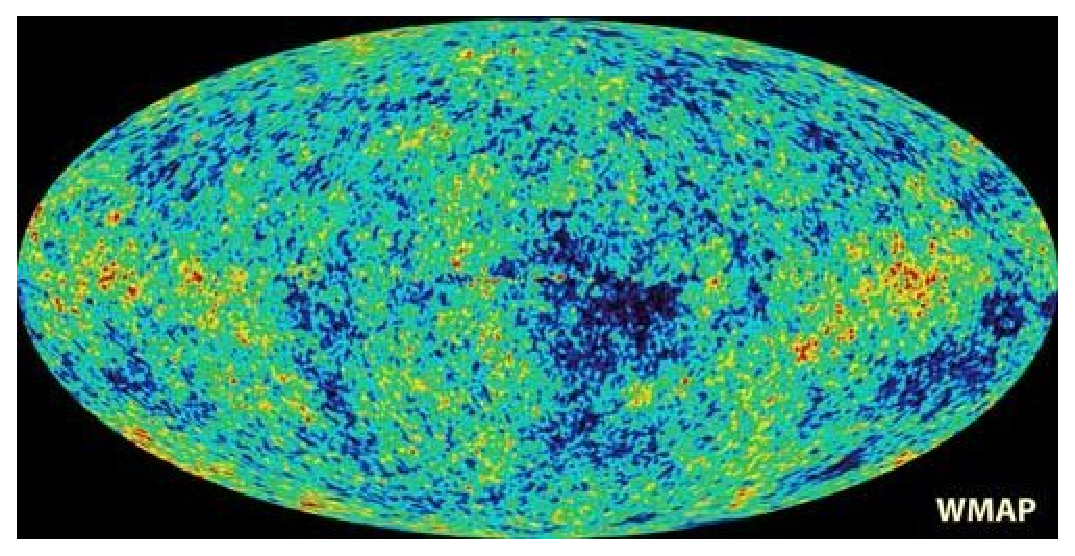
\includegraphics[width=1.8in]{pictures/wmap.eps}}
				\end{minipage}
			\end{tabular}
		\end{itemize}
	}
	}
	}
}}
}


